% Manual Técnico

% Configuración
\documentclass[a4paper,12pt]{book}

\usepackage[utf8]{inputenc}
\usepackage[spanish]{babel}
\usepackage[top=3cm,bottom=3cm,left=3.5cm,right=2cm]{geometry}
\usepackage{fancyhdr}
\usepackage[bookmarksnumbered=true,pdfborder={0 0 0},colorlinks=true,
            linkcolor=blue,urlcolor=blue,citecolor=blue]{hyperref}
\usepackage[final]{pdfpages}
\usepackage[nottoc]{tocbibind}
%

% Detalles
\author{Bartolomé Sánchez Salado}
\title{Asesorías Académicas}
\date{\today}
%

% Cabeceras
\pagestyle{fancy}
\headheight 16pt
\lhead{\nouppercase{\rightmark}}
\rhead{\nouppercase{\leftmark}}
%

% Arreglo de los márgenes de las subsecciones
\usepackage[titles]{tocloft}
\cftsetindents{subsection}{1.9em}{3.5em}
\cftsetpnumwidth{1.8em}

% Quitar cabecera y pie de página a las páginas en blanco
\let\origdoublepage\cleardoublepage
\newcommand{\clearemptydoublepage}{%
  \clearpage
{\pagestyle{empty}\origdoublepage}%
}
\let\cleardoublepage\clearemptydoublepage
%

\begin{document}

   \pagenumbering{alph}

   \begin{titlepage}
      \maketitle
   \end{titlepage}

   \setcounter{page}{0}
   \cleardoublepage

   \pagenumbering{roman}
   \tableofcontents

   \chapter{Introducción}
   \pagenumbering{arabic}
      \subsection{Asesorías Académicas}

\paragraph{}La asesoría es una acción docente de orientación con la finalidad de
participar en la formación integral del alumno, potenciando su desarrollo
académico y personal, así como su proyección social y profesional.

\paragraph{}La forma de expresión clásica de asesoría docente en el ámbito
universitario se limitaba a las Tutorías Académicas. Este tipo de asesoría,
inherente al rol de profesor, la realiza cada docente en su asignatura con su
grupo de estudiantes. En ellas los profesores supervisan el trabajo del
estudiante, orientan, resuelven dudas, aconsejan bibliografía, revisan trabajos
y pruebas, etc., pero siempre dentro del ámbito de la propia asignatura. Por su
parte, como se ha indicado anteriormente, la asesoría académica tiene una
aplicación más amplia y genérica.

\paragraph{}Con el fin de aumentar la calidad en la enseñanza dentro del ámbito
universitario, aparece la figura del Asesor Académico. Su labor sería la
de orientar e informar al estudiante sobre cualquier duda en relación con los
aspectos académicos que se le puedan plantear durante su estancia en la
Universidad, a través de un seguimiento permanente, eficaz y orientado a la
optimización del esfuerzo de estudio por parte del alumnado.

\paragraph{}La Universidad de Córdoba, con el fin de garantizar y satisfacer el
ejercicio de un derecho reconocido a los estudiantes, como es la labor de
asesoría docente, y mejorar el rendimiento académico del alumnado, muy bajo en
un buen número de las titulaciones que se imparten en ella, aprobó en marzo de
2007 por el Consejo de Gobierno el Plan Propio de Calidad de la Enseñanza, donde
se contempla la creación de la figura del Asesor Académico.

\paragraph{}Para llevar a cabo su implantación, la Universidad establece un
reglamento regulador que define el papel del asesor académico; además, con la
intención de facilitar la organización y el seguimiento, se proporcionan una
serie de guías y fichas donde el docente gestionará su relación con cada uno de
los alumnos a los que asesore.

\paragraph{}Dada la complejidad que supone gestionar toda la información
relativa a la Asesoría Académica, más para el docente aunque algo también para
el alumno, y lo reciente de su implantación, hace ineficiente el normal
desarrollo de la actividad de asesoría. El proyecto fin de carrera que se desea
realizar pretende superar estas dificultades; proporcionando, a todos los
implicados en la actividad de asesoría, un sistema informático que facilite la
gestión y el mantenimiento de la información relativa a la Asesoría Académica.

      \subsection{Definición del problema real}

Debido a la reciente implantación del rol del asesor académico en el entorno
universitario de la Universidad de Córdoba, resulta tediosa y poco eficiente la
tarea de organizar la información relativa a la relación alumno-asesor para
cada una de las dos partes.

La Universidad ha proporcionado una serie de documentos (consejos
generales, fichas de seguimiento, encuestas, guías de reuniones, etcétera.) con
el objetivo de que los asesores puedan llevar cierto control sobre los alumnos
a los que imparten asesoría. Este método conlleva varias deficiencias:

\begin{itemize}
 \item Toda la gestión y control de la información se realiza sobre papel, lo
       que no resulta eficiente en el caso de disponer de una gran cantidad de
       alumnos a los que impartir asesoría; además, no es difícil que algún
       folio se extravíe.
 \item Imposibilidad de compartir información públicamente (siempre que ésta
       de verdad quiera ser compartida). Esto conlleva, por ejemplo, a que un
       alumno no puede, en principio, conocer qué profesores se ofrecen, en un
       momento determinado, a prestar servicio de asesoría.
 \item Resulta muy problemática la actualización o modificación de cualquier
       elemento de la información que sea necesario corregir. Como sabemos, los
       métodos de corrección de la escritura tradicional no son todo lo
       efectivos o limpios que nos gustaría.
\end{itemize}

El sistema que se pretende desarrollar persigue resolver estos problemas así
como facilitar la gestión y manipulación de toda la información relativa a
las Asesorías Académicas, además de aprovechar las ventajas que suponen hoy en
día las tecnologías de la información, como pueden ser:

\begin{itemize}
 \item Fácil acceso a la información. En la actualidad y cada día más, muchas
       personas tienen acceso a internet, a través de múltiples dispositivos y
       en diversos lugares.
 \item Almacenamiento de grandes cantidades de información, así como su posible
       centralización.
 \item Fácil manipulación de los datos almacenados.
 \item Interactividad. Se fomenta la relación alumno-asesor a través de
       múltiples formas ( correo electrónico, foros, etc. ).
\end{itemize}

      \section{Problema Técnico}

\paragraph{}A partir de las características del problema real, pueden extraerse
una serie de condicionantes técnicos que influirán de forma decisiva en el
producto final. Para la obtención de éstos, se va a utilizar una técnica de
ingeniería denominada PDS (Product Design Specification). Los siguientes
elementos determinan las especificaciones técnicas que caracterizan al problema.

\begin{itemize}
 \item Funcionamiento

   \paragraph{}La aplicación permitirá la gestión y el mantenimiento de la
   información relativa a la Asesoría Académica; es decir, información personal
   de los alumnos asesorados así como el seguimiento de los mismos a lo largo
   de la labor de asesoría.

   \paragraph{}El sistema dispondrá de la información personal necesaria de
   alumnos con el objetivo de de facilitar el trabajo de la labor de asesoría a
   quienes la realizan. A su vez, se proporcionará a los asesores herramientas
   que faciliten un seguimiento exhaustivo de cada uno de los alumnos
   asesorados.

   \paragraph{}Además se dispondrá de un generador de informes donde se podrán
   realizar consultas y elaborar documentos personalizados a partir de
   determinados parámetros de entrada. Todo documento generado tendrá la
   capacidad de ser parametrizado; es decir, será relativamente manipulable
   para que pueda ser modificado o actualizado según sea preciso.

   \textit{\paragraph{}Por otra parte, la aplicación permitirá a los asesores
   crear entrevistas (individuales o grupales), personalizables o elegidas a
   través de una serie de plantillas, que serán contestadas por los alumnos.
   ¿¿Mediante la propia aplicación??.}

   \paragraph{}Finalmente, para evitar pérdidas de información existente
   en el sistema, y mantener una apropiada integridad de la misma, la aplicación
   permitirá hacer copias de seguridad.

   \paragraph{}En el capítulo \ref{espReq}, \textit{Especificación de
   requisitos}, se encuentran reflejadas con más detalle las funciones del
   sistema.

 \item Entorno

   \paragraph{}El sistema a desarrollar consistirá en una aplicación web alojada
   en un servidor, a la que los usuarios accederán a través de Internet o red
   local mediante el uso de un navegador.

   \paragraph{}La aplicación constará de una interfaz amigable e
   intuitiva basada en cuadros de diálogo, botones, menús desplegables, etc.
   Como periféricos de entrada, serán necesarios el teclado y el ratón. Como
   periféricos de salida, la impresora. Para la generación de determinados
   informes, como los correos electrónicos, será necesaria la conexión a
   Internet.

 \item Vida esperada

   \paragraph{}Este sistema, en principio, no tiene una vida esperada
   determinada. El tiempo de funcionamiento debería ser el máximo posible,
   siempre que su utilización suponga alguna ventaja sustancial con respecto a
   otros futuros sistemas alternativos.

   \paragraph{}Debido a los cambios administrativos que se pueden dar en los
   centros universitarios, como por ejemplo, la incorporación de nuevas
   titulaciones o el cambio de planes de estudios, este sistema tendrá que ser
   continuamente revisado para mantenerlo actualizado a los cambios producidos.

 \item Ciclo de mantenimiento

   \paragraph{}Debido a que el sistema informático va a ser desarrollado como
   objetivo de un proyecto de fin de carrera, se considera que el autor no debe
   ser el responsable de su mantenimiento. No obstante, en su realización, se
   utilizará una metodología de desarrollo modular que permite a otros
   programadores incorporar futuras mejoras con facilidad.

 \item Competencia

   \paragraph{}Debido a la reciente implantación del rol del asesor académico,
   no se conoce ningún sistema de software dentro de la Universidad de Córdoba
   ni en el resto de universidades que realice las funciones desempeñadas por
   éste.

 \item Aspecto externo

   \paragraph{}El sistema constará de una interfaz intuitiva y ergonómica que
   hará que su uso sea cómodo y fácil. Ésta constará de elementos bien conocidos
   y comúnmente utilizados como cuadros de diálogo, botones, menús desplegables,
   etc.

   \paragraph{}El soporte utilizado para albergar la aplicación será el CD-ROM,
   por ser ampliamente utilizado, compatible y de tamaño suficiente.

   \paragraph{}El aspecto externo se encuentra explicado con más detalle en el
   capítulo \ref{espReqInt}, \textit{Especificación de requisitos de la
   interfaz}.

 \item Estandarización

   \paragraph{}El sistema de software a desarrollar mantendrá un alto nivel de
   estandarización en cuanto a:

   \begin{itemize}
      \item Sistema de almacenamiento de información. El motor de la base de
      datos utilizado para albergar la información está ampliamente implantado
      en el mercado. Dicho sistema de almacenamiento se denomina MySQL.
      \item Interfaz de ventanas. Se hará uso de instrumentos de diseño de
      interfaz muy populares, los cuales se encuentran expuestos en el capítulo
      \ref{recursos}, Recursos.
      \item Soporte digital CD-ROM.
   \end{itemize}


 \item Calidad y fiabilidad

   \paragraph{}La aplicación comprobará los pasos dados por el usuario: si en
   algún momento éste realiza una acción no permitida, el sistema intentará
   guiarle mediante mensajes de ayuda.

 \item Pruebas

   \paragraph{}Las pruebas realizadas sobre el sistema son un elemento
   determinante a la hora de garantizar la calidad y fiabilidad del mismo.

   \paragraph{}Para comprobar que el sistema funciona correctamente, estas
   pruebas tendrán dos objetivos básicamente:

   \begin{itemize}
      \item Comprobar que la aplicación hace lo que debe hacer.
      \item Probar que la aplicación no hace lo que no debe hacer, es decir,
      comprobar que no provoca efectos secundarios adversos.
   \end{itemize}

   \paragraph{}Se realizarán pruebas sobre los siguientes subsistemas de la
   aplicación:

   \begin{itemize}
      \item Interfaz: comprobando el correcto funcionamiento de los diferentes
      componentes que la constituyen.
      \item Comunicación con la base de datos del sistema y la apropiada
      modificación de la información que alberga.
      \item Generación de documentos y parametrización de los mismos.
      \item Instalación y desinstalación.
   \end{itemize}

   Las pruebas realizadas sobre este nuevo sistema de software se
   encuentran detalladas en el capítulo \ref{pruebas}, \textit{Pruebas}.


 \item Seguridad

   \paragraph{}El sistema de gestión de bases de datos de la aplicación tiene la
   capacidad de proteger los datos contra su pérdida parcial o total debidos a
   fallos en el sistema. A su vez, garantiza la privacidad, es decir, sólo
   permite el acceso a la información a personas autorizadas.

   \paragraph{}Dependiendo de quién acceda o use la base de datos, se le
   mostrará una visión diferente de los datos que sea capaz de reconocer,
   interpretar y manejar. De esta manera tenemos varias visiones diferentes. La
   que poseerán los alumnos, la que poseerán los profesores, y finalmente la del
   administrador. Estas visiones   particulares son proporcionadas por los
   programas de aplicación que manejan sólo parte de la información contenida
   en la base de datos.


   \paragraph{}Finalmente, el mecanismo de copias de seguridad del sistema
   permitirá al usuario salvaguardar la información siempre que crea
   conveniente.

\end{itemize}


   \chapter{Objetivos}
      \section{Objetivo principal}

\paragraph{}El objetivo principal de la realización de este proyecto será el
desarrollo e implantación de un sistema de software que facilite a los usuarios
implicados en las Asesorías Académicas (asesores y alumnos) la gestión y
mantenimiento de la información relativa a la Asesoría Académica.

\paragraph{}Este sistema debe permitir el acceso de manera personalizada a la
información que en él se almacena; por tanto, se hace necesario distinguir entre
los distintos tipos de usuarios que accederán al sistema en cuestión, que serán:

\begin{itemize}
 \item Usuario administrador.
 \item Usuario asesor.
 \item Usuario alumno.
\end{itemize}

\paragraph{}Esto implica que, a la hora de acceder al sistema, se deba realizar
una identificación para conocer al usuario que desea acceder y poder ofrecerle
los servicios que, para su tipo de usuario y para ese usuario en concreto, han
sido establecidos.

\paragraph{}El usuario administrador será el encargado de gestionar el resto de
usuarios del sistema, mientras que los usuarios asesor y alumno deberán poder
acceder a la información que les pertenece y realizar las acciones que sean de
su incumbencia.
      \section{Objetivos secundarios}

\paragraph{}Para alcanzar nuestro objetivo principal, se han de alcanzar unos
objetivos secundarios, que tienen su importancia para el desarrollo de la
aplicación. Estos objetivos son los siguientes:

\begin{itemize}
   \item Diseñar una base de datos que permita la gestión de toda la información
         de interés relativa a la Asesoría Académica para cada curso académico:
   \begin{itemize}
      \item Asesores.
      \item Alumnos: datos académicos y personales.
      \item Seguimiento de la asesoría: entrevistas, rendimiento académico, etc.
      \item Organización docente: centros, titulaciones, asignaturas.
      \item Etc.
   \end{itemize}

   \item Realizar un desarrollo de la aplicación modular que permita satisfacer
         las necesidades de cada uno de los tipos de usuarios:
   \begin{itemize}
      \item Administrador principal.
      \item Administrador de centro.
      \item Asesor académico.
      \item Alumno.
   \end{itemize}

   \item Crear un entorno interactivo robusto, consistente, amigable, intuitivo,
         de fácil manejo que fomente la interacción entre los usuarios y la
         interfaz, en la que se incluirán todas las opciones necesarias para
         cada uno de los tipos de usuario existente en la aplicación.

   \item Proporcionar una aplicación con unos mecanismos de control de acceso
         para garantizar la privacidad, seguridad e integridad de la
         información.

   \item Potenciar la explotación del sistema, facilitando las consultas sobre
         las asesorías académicas.
\end{itemize}


\paragraph{}Se pretende que el sistema a desarrollar ofrezca una serie de
funcionalidades para cada tipo de usuario, con el objetivo de satisfacer las
necesidades de cada uno de ellos. A continuación se detallan las características
que se esperan alcanzar para cada uno de los usuarios del sistema.


\begin{itemize}
   \item Características comunes a todos los usuarios del sistema.
      \begin{itemize}
         \item Todos los usuarios podrán ejecutar consultas, de forma que, a
         través de una serie de condiciones de entrada, se genere una salida que
         satisfaga dichos valores.
         \item La parametrización de todo documento emitido por la aplicación.
         Esta función del sistema va a ser de gran importancia, ya que permitirá
         que los documentos sean modificados o actualizados según sea
         conveniente.
      \end{itemize}

   \item Características del usuario administrador principal.
      \begin{itemize}
         \item Tendrá la posibilidad de gestionar al resto de usuarios del
               sistema.
         \item Establecerá los distintos centros que presente el sistema,
               designando su respectivo usuario administrador de centro.
         \item Podrá establecer y mantener los diferentes planes docentes que el
               sistema soportará.
         \item Le estará permitido administrar las distintas plantillas
         que podrán ser usadas para generar entrevistas.
         \item Podrá generar informes del estado de usuarios del sistema, que
         puedan ser mostrados por pantalla o imprimidos.
         \item Podrá efectuar copias de seguridad, para salvaguardar cuando
         desee la información existente en el sistema.
      \end{itemize}

   \item Características del usuario administrador de centro.
      \begin{itemize}
       \item Posibilidad de gestionar a los usuarios pertenecientes al centro
             que le concierne, tanto asesores como alumnos.
       \item Podrá establecer y mantener los diferentes planes docentes de los
             que su centro disponga.
       \item Por defecto en el sistema, será el encargado de relacionar los
             distintos usuarios asesores con sus correspondientes alumnos,
             asignando a cada usuario alumno el asesor que le corresponda. Esta
             opción, no obstante, podrá ser reemplazada por otras dos
             posibilidades, que serán comentadas con mayor profundidad más
             adelante:
             \begin{itemize}
               \item El usuario asesor se autoasigna sus usuarios alumnos.
               \item El usuario alumno elige a su usuario asesor.
             \end{itemize}
             Estas opciones no podrán activarse simultáneamente en el sistema,
             debiendo elegirse únicamente una de las tres posibilidades.
      \end{itemize}

   \item Características del usuario asesor.
      \begin{itemize}
         \item Tendrá la posibilidad de visualizar y modificar su información
         personal.
         \item Se permitirá a cada asesor gestionar la información de sus
         alumnos de forma fácil e intuitiva.
         \item Deberá permitir realizar un seguimiento de cada alumno en
         particular.
         \item Podrá generar informes de información personal de alumnos y su
         seguimiento, que podrán ser mostrados por pantalla o imprimidos.
         \item Un asesor podrá generar entrevistas, grupales o individuales, que
         podrán ser mostradas por pantalla o imprimidas, las cuales, además,
         podrán ser recibidas por los alumnos a través del correo electrónico.
         \item Dispondrá de dos funcionalidades, desactivadas por defecto,
         respecto a la forma en que se relaciona con el usuario alumno:
         \begin{itemize}
            \item Será el encargado de autoasignarse sus propios usuarios
            alumnos a los que ofrece asesoría.
            \item Podrá validar a los usuarios alumnos que les pidan asesoría.
         \end{itemize}
      \end{itemize}

   \item Características del usuario alumno.
      \begin{itemize}
         \item Tendrá la posibilidad de visualizar y modificar su información
         personal.
         \item Como opción desactivada por defecto, podrá visualizar los
         asesores disponibles para prestar asesoría así como solicitar sus
         servicios, en caso de no tener asignado uno previamente.
      \end{itemize}
\end{itemize}



   \chapter{Antecedentes}
      \paragraph{}El Consejo de Gobierno de la Universidad de Córdoba de 27 de junio
de 2008 acordó la aprobación del Reglamento regulador de la figura del Asesor
Académico\footnote{Acuerdo del Consejo de Gobierno de 27 de junio de 2008, por
el que aprueba el Reglamento regulador de la figura del Asesor Académico.
Universidad de Córdoba. Ver Apéndice \ref{a1}.}. En dicho reglamento se
establecen las competencias de los asesores académicos así como el proceso de
asignación de los estudiantes asesorados.

\paragraph{}De dicho reglamento se destacan las siguientes cuestiones:

\begin{itemize}
   \item \textit{``En cada Centro, bajo la responsabilidad de su Dirección,
   existirá una lista o registro de Asesores Académicos, en el que se podrán
   inscribir todos aquellos profesores adscritos al Centro que quieran ejercer
   funciones de asesoría académica.}
   \item \textit{``En el momento de formalizar su primera matrícula, a cada
   estudiante se le informará sobre la figura del Asesor Académico y se le
   asignará uno de los inscritos en la lista o registro del Centro.''}
   \item \textit{``Cada Asesor Académico tendrá a su cargo un máximo de 25
   estudiantes.''}
   \item \textit{``El Asesor tendrá a su cargo a los estudiantes que se le
   asignen durante el tiempo que permanezcan en la titulación, es decir, desde
   su ingreso hasta que finalicen sus estudios o los abandonen.''}
   \item \textit{``En la segunda y sucesivas matrículas, y antes de cada proceso
   de matriculación, el Asesor, por iniciativa de éste, tendrá una entrevista
   con sus estudiantes asignados. Asimismo, el Asesor deberá entrevistarse con
   los estudiantes asignados al menos una vez cada cuatrimestre.''}
   \item \textit{``El Asesor deberá aceptar las peticiones debidamente
   fundamentadas de entrevista por parte de sus estudiantes en cualquier momento
   del curso. Asimismo, podrá convocar a todos o a parte de ellos cuando lo crea
   conveniente.''}
   \item \textit{``El Asesor tendrá un historial de cada uno de sus estudiantes
   (incluyendo una fotografía reciente de los mismos y datos de contacto postal,
   telefónico y por Internet) en el que figurarán sus recomendaciones,
   comentarios y aquellos aspectos que considere de interés.''}

   \item \textit{``Los Asesores Académicos y los vicedecanos o
   subdirectores que ejerzan funciones de tutoría actuarán coordinadamente,
   siguiendo las directrices que al respecto apruebe el Director o Decano del
   Centro. Los Asesores se reunirán con la Dirección del Centro un mínimo de dos
   veces al año, para hacer un seguimiento de la labor realizada.``}

\end{itemize}
      \section{Aplicaciones informáticas}

\paragraph{}Como aplicaciones informáticas que resuelvan, o traten de resolver,
el mismo problema que el planteado por el presente documento, se conoce
únicamente la aplicación \textit{Portal para la asesoría académica}
\cite{carmonaVaro}.

\paragraph{}Dicha aplicación, tiene su razón de ser como \textit{herramienta que
permita el almacenamiento y la gestión de las reuniones de asesoría, que sea de
gestionar la asignación de asesores y alumnos en la formación de grupos de
asesoría y que facilite la comunicación con estos,} (sic) \textit{permitiendo la
compartición de documentos de interés e información relevante para los alumnos y
facilitando información a los asesores sobre el seguimiento de los alumnos.
Además se persigue poder ofrecer tanto a alumnos como a asesores una serie de
encuestas para evaluar la actividad.}

\paragraph{}Para su consecución hace uso de un sistema de gestión de contenidos
(CMS, \textit{Content Management System}) denominado Joomla! \cite{joomla},
debido a que \textit{permiten descentralizar las labores del mantenimiento del
contenido de un portal, de forma que el personal no técnico de los distintos
departamentos de una empresa pueda añadir, editar y gestionar su propio
contenido en una web.}

\paragraph{}El principal problema de esta aplicación es que no resuelve el
problema de gestionar con eficacia la información relativa a las asesorías
académicas:

\begin{itemize}
 \item En ella no se tienen en cuenta ni los centros, ni las titulaciones, ni
       las asignaturas a las que pertenecen tanto asesores como alumnos, lo que
       provoca que la información generada resulte muy desorganizada, además de
       escasa. Por ejemplo, no es posible que un asesor conozca las asignaturas
       aprobadas o pendientes de un determinado alumno al que preste asesoría,
       algo esencial a la hora de poder orientarlo correctamente.
 \item Tampoco se tienen en cuenta diferentes cursos académicos, lo que provoca
       que la información siempre parezca actual, complicando un más que
       deseable estudio de la evolución temporal de los acontecimientos. Esto
       significa que un asesor, por ejemplo, pueda conocer cuántas asignaturas
       aprueba un alumno anualmente, para poder recomendarle mejor a la hora
       de efectuar la siguiente matriculación.
 \item Por otro lado, no es posible distinguir entre las preguntas oficiales
       proporcionadas por el Vicerrectorado para la asesoría académica de las
       posibles preguntas personales que pueda necesitar realizar un profesor.
       Por lo tanto, en dicha aplicación todas las preguntas son preguntas del
       sistema, por lo que los asesores no disponen de la libertad de generar
       sus propias preguntas personales para realizarlas a los alumnos a los que
       preste asesoría.
\end{itemize}
      \paragraph{}El Vicerrectorado de Planificación y Calidad de la Universidad de
Córdoba ha emitido una serie de fichas de información personal y de seguimiento,
individual y grupal, de los estudiantes asesorados con el objeto de que los
asesores tengan cierto control y organización durante la labor de asesoría.

\paragraph{}Esto supone que cada asesor es responsable directo de su propia
organización con respecto a la información relativa a los estudiantes
asesorados, pudiendo hacer uso de estas fichas, las cuales, sirven como guía.

\paragraph{}Si tenemos en cuenta que el Reglamento regulador de la figura del
Asesor Académico dispone que ``los asesores que ejerzan funciones de tutoría
actuarán coordinadamente'', se percibe como una mala idea que cada asesor se
organice a su manera.

\paragraph{}Para solucionar este problema, se hace necesario desarrollar un
sistema de software que centralice toda la información que los asesores
necesiten disponer y que facilite la labor de asesoría con respecto a sus
alumnos.


   \chapter{Restricciones}
      \section{Factores Iniciales}

\paragraph{}Observando la naturaleza del problema que se pretende resolver, se
tienen en cuenta los siguientes factores iniciales:

\begin{itemize}
   \item Se deberá realizar un sistema de software que gestione la información
   relativa a la Asesoría Académica.
   \item Este sistema debe ser accesible por red como servicio web, ya sea a
   través de una red local o internet; y, por tanto, multiplataforma.
   \item Para su funcionamiento interno, se hará uso de una base de datos que
   gestione la información existente.
   \item Por otra parte, permitirá la realización copias de seguridad de la
   información existente en el sistema.
\end{itemize}

      \section{Factores estratégicos}

\paragraph{}En cuanto a las características técnicas, se han decidido como
factores estratégicos, para la consecución de este proyecto, los siguientes:

\begin{itemize}
   \item El sistema operativo que se utilizará para el desarrollo del proyecto
   será Debian GNU/Linux 6.0 (INSERTAR CITA), por ser éste el sistema habitual
   del desarrollador principal y estar claramente familiarizado con él.
   \item Se ha decidido utilizar un sistema de control de versiones para el
   desarrollo del proyecto, abarcando tanto la documentación como la generación
   de código, con el objetivo de facilitar la administración de los elementos
   que se generen a medida que evolucionan. La aplicación software encargada de
   éste cometido elegida se denomina Subversion (INSERTAR CITA), por varias
   razones, entre las que se encuentran:
   \begin{itemize}
      \item Es software libre.
      \item Fácil de instalar en el sistema operativo sobre el que se trabaja.
      \item Bastante documentación existente y de fácil acceso.
   \end{itemize}
   \item Para el funcionamiento de la base de datos, se ha decidido utilizar
   MySQL 5.0(INSERTAR CITA). Entre los motivos se encuentran el ser software
   libre y la fácil instalación/configuración en el sistema operativo sobre el
   que se desarrolla la aplicación.
   \item Al ser un servicio web, el contenido generado por la aplicación deberá
   hacer uso del lenguaje de marcado HTML, o alguna de sus variantes (XHTML), al
   ser el lenguaje de marcado estándar.
   \item Para la generación de contenido, se hará uso de un lenguaje del lado
   del servidor. Se ha decidido utilizar PHP/Ruby(On Rails)/Python(Django) por
   el motivo X.
\end{itemize}

\paragraph{}En lo que respecta a funcionalidades de la aplicación, se han tomado
las siguientes decisiones:

\begin{itemize}
   \item Cada usuario podrá acceder al sistema de forma personalizada; es decir,
   a través de un sistema de identificación personal. La información manejada
   por cada usuario es particular, y dependiente del rol que desempeñe.
   \item Las entrevistas generadas por los asesores se podrán hacer llegar a los
   alumnos mediante correo electrónico.
   \item La interfaz gráfica a usar deberá ser de fácil manejo e intuitiva,
   basada en elementos gráficos usados comúnmente como por ejemplo: cuadros de
   texto, botones, etiquetas, etc.
\end{itemize}



   \chapter{Recursos}\label{recursos}
      \section{Software}

   \paragraph{}La mayoría de las aplicaciones que a continuación se detallan,
   o bien han sido justificadas en el apartado \ref{facEst}, \textit{Factores
   estratégicos}, o bien se justifican llegado el momento.

   \subsection{Sistemas operativos}

      \subsubsection{Sistema operativo de desarrollo}

      \paragraph{}Para el desarrollo del sistema, incluyendo la documentación,
      se va a disponer del siguiente sistema operativo:

      \begin{itemize}
         \item Nombre: Debian GNU/Linux \cite{debian}.
         \item Versión: 6.0 (Squeeze).
         \item Descripción: Sistema operativo basado en software libre.
         \item Disponibilidad: Toda la duración del proyecto.
         \item Tiempo de utilización: Toda la duración del proyecto.
      \end{itemize}

      \subsubsection{Sistema operativo servidor de aplicaciones}

      \paragraph{}El servidor que actuará como sistema de control de versiones
      utiliza el mismo sistema operativo pero una versión inferior, 5.0 (Lenny),
      con las mismas condiciones de disponibilidad y tiempo de utilización que
      el expuesto anteriormente.

   \subsection{Editores}

      \subsubsection{Editores de documentación}

      \paragraph{}A la hora de generar la documentación, se hará uso de la
      aplicación Latex, que se detalla a continuación:

      \begin{itemize}
         \item Nombre: Latex \cite{latex}.
         \item Versión: LaTeX2e.
         \item Descripción: Lenguaje de marcado y preparación de documentos.
         \item Disponibilidad: Toda la duración del proyecto.
         \item Tiempo de utilización: Durante la documentación.
         \item Justificación: Son varios los motivos para realizar la
         documentación en este lenguaje, entre los que destacan:
            \begin{itemize}
               \item Permite estructurar documentos fácilmente.
               \item Alta calidad tipográfica.
               \item Gran cantidad de paquetes externos disponibles que
               potencian el lenguaje.
               \item Posibilidad de realizar un mantenimiento de los elementos
               generados a través del control de versiones.
            \end{itemize}
      \end{itemize}

      \paragraph{}Para generar el código fuente que necesita Latex, se utilizará
      un editor, que se expone seguidamente:

      \begin{itemize}
         \item Nombre: Kile \cite{kile}.
         \item Versión: 2.0.85.
         \item Descripción: Editor de TeX/LaTeX.
         \item Disponibilidad: Toda la duración del proyecto.
         \item Tiempo de utilización: Durante la documentación.
         \item Justificación: Esta aplicación facilita la edición de texto en
         Latex.
      \end{itemize}

      \subsubsection{Editores de código}

      \paragraph{}La edición del código fuente se realizará utilizando la
      aplicación Kate, que seguidamente se detalla:

      \begin{itemize}
         \item Nombre: Kate \cite{kate}.
         \item Versión: 3.4.5.
         \item Descripción: Editor de textos avanzado.
         \item Disponibilidad: Toda la duración del proyecto.
         \item Tiempo de utilización: Durante la codificación.
         \item Justificación: Esta aplicación facilita la edición de texto
               en lenguaje Python.
      \end{itemize}

   \subsection{Lenguajes de programación}

   \paragraph{}Como se comentó anteriormente en el apartado \textit{Factores
   estratégicos} \ref{facEst}, el lenguaje de programación a utilizar será
   Python, haciendo uso del \textit{framework} de desarrollo Django.

   \subsection{Servidores}

      \subsubsection{Sistema de control de versiones}

         \begin{itemize}
            \item Nombre: Subversion \cite{subversion}.
            \item Versión: 1.4.2.
            \item Descripción: Software de sistema de control de versiones.
            \item Disponibilidad: Toda la duración del proyecto.
            \item Tiempo de utilización: Toda la duración del proyecto.
         \end{itemize}

      \subsubsection{Sistema gestor de bases de datos}

         \begin{itemize}
          \item Nombre: PostgreSQL \cite{postgresql}.
          \item Versión: 8.4.5.
          \item Descripción: Sistema de gestión de base de datos relacional.
          \item Disponibilidad: Toda la duración del proyecto.
          \item Tiempo de utilización: Toda la duración del proyecto.
         \end{itemize}

      \subsection{Servidor web}

         \begin{itemize}
          \item Nombre: Apache \cite{apache}.
          \item Versión: 2.2.16-4.
          \item Descripción: Servidor web HTTP.
          \item Disponibilidad: Toda la duración del proyecto.
          \item Tiempo de utilización: Toda la duración del proyecto.
         \end{itemize}

      \section{Hardware}

\begin{itemize}
   \item Ordenador personal Intel Pentium 4 CPU 2.40Ghz, con 768MB de memoria
   RAM y disco duro de 30GB como principales características, utilizado para el
   desarrollo del proyecto.
   \item Ordenador personal Intel Celeron CPU 800Mhz, con 256MB de memoria RAM y
   disco duro de 40GB como principales características, utilizado como servidor
   del gestor de versiones del desarrollo del proyecto.
\end{itemize}
      \subsection{Humanos}

Prueba de recursos humanos.


   \chapter{Especificación de requisitos}\label{espReq}
      \section{Introducción}

  \paragraph{}En este capítulo se muestra una visión detallada del
  comportamiento del sistema de manera que sea entendible tanto por el usuario
  final como por los desarrolladores, mediante una representación de cómo fluye
  la información por el sistema desde su entrada hasta su salida.

  \paragraph{}Para realizar esta representación, se utilizarán una serie de
  Diagramas de Flujo de Datos (DFD) que son una herramienta que permite
  visualizar un sistema como una red de procesos funcionales, conectados entre
  sí por \textit{conductos} y \textit{tanques de almacenamiento} de datos.
  También se utilizará un Diccionario de Datos que realizará una representación
  de los elementos requeridos o producidos por la aplicación.

      \section{Descripción Modular}

\paragraph{}

\begin{itemize}
   \item Datos Personales.
   \begin{itemize}
      \item \textit{¿Fotografía.?}
      \item D.N.I.
      \item Fecha de nacimiento.
      \item Nombre.
      \item Apellidos.
      \item Dirección en Córdoba.
      \item Teléfonos.
      \item Correo electrónico.
      \item Residencia durante el curso.
   \end{itemize}
   \item Datos Familiares.
   \begin{itemize}
      \item Dirección familiar.
      \item Localidad.
      \item Código postal.
      \item Provicia.
      \item Teléfonos.
   \end{itemize}
   \item Datos Académicos.
   \begin{itemize}
      \item Estudios realizados en año pasado.
      \item Estudios que está realizando.
      \item Curso.
      \item Año de ingreso en la Universidad.
      \item Otros estudios universitarios.
      \item Modalidad de acceso a la universidad.
      \item Calificación de: acceso/estudios previos.
   \end{itemize}
\end{itemize}


\paragraph{}Para llevar a cabo el seguimiento de los alumnos, el sistema deberá
poder gestionar la siguiente información:

\begin{itemize}
   \item Datos de la reunión.
   \begin{itemize}
      \item Asesor.
      \item Alumno (en caso de seguimiento individual).
      \item Asistentes (en caso de seguimiento grupal).
      \item Fecha.
      \item Hora.
      \item Duración.
   \end{itemize}
   \item Motivo.
   \item Orientaciones realizadas.
   \item Observaciones.
   \item Próxima reunión, temas a tratar.
   \begin{itemize}
      \item Fecha.
      \item Hora.
   \end{itemize}
\end{itemize}

      \section{Supuestos Semánticos}

   \paragraph{}A continuación se detallan las entidades que participan en el
   diseño del sistema, con sus correspondientes supuestos semánticos.

   \begin{description}

      \item[Titulación] Conjunto de materias cuya superación supone la obtención
      de un título académico.
      \begin{itemize}
         \item Cada titulación tiene un identificador que hace referencia a ella
          de forma unívoca.
          \item Una titulación está compuesta de al menos una asignatura y como
         máximo un número indeterminado.
      \end{itemize}

      \item[Asignatura] Materia que forma parte del plan de estudios de una
      titulación.
      \begin{itemize}
         \item Cada asignatura tiene un identificador que hace referencia a ella
         de forma unívoca.
         \item Una asignatura pertenece a una y solo a una titulación.
         \item \textit{Una asignatura pertenece a una o a varias áreas de
         conocimiento.}
         \item Una asignatura tiene asignada una carga docente traducida en
         un número de créditos.
         \item \textit{Los créditos de una asignatura pueden estar compuestos de
         créditos teóricos, prácticos y/o problemas.}
         \item Una misma asignatura se puede impartir en varios cursos
         académicos.
      \end{itemize}

      \item[Curso académico] Tiempo señalado en cada año en el que se imparte
      docencia.
      \begin{itemize}
         \item Cada curso académico tiene un identificador que hace referencia
         al mismo de forma unívoca.
         \item En un curso académico se imparte al menos una y como máximo
         un número indeterminado de asignaturas.
         \item Un número indeterminado de alumnos pertenece a un determinado
         curso académico.
      \end{itemize}

      \item[Alumno] Estudiante de una titulación que recibe asesoría.
      \begin{itemize}
         \item Cada alumno tiene un identificador que hace referencia al mismo
         de forma unívoca.
         \item Un alumno recibe asesoría de un, y solo un, asesor.
         \item Un determinado alumno puede estar matriculado en un número
         indeterminado de cursos académicos.
      \end{itemize}

      \item[Asesor] Tutor que realiza un seguimiento permanente y orientado a la
      optimización del esfuerzo de estudio de un alumno.
      \begin{itemize}
         \item Cada asesor tiene un identificador que hace referencia al mismo
         de forma unívoca.
         \item Un asesor asesora a un número indeterminado de alumnos.
      \end{itemize}

 \end{description}


   \chapter{Modelo Entidad-Interrelación}\label{modEntInt}
      \section{Introducción}

  \paragraph{}En este capítulo se muestra una visión detallada del
  comportamiento del sistema de manera que sea entendible tanto por el usuario
  final como por los desarrolladores, mediante una representación de cómo fluye
  la información por el sistema desde su entrada hasta su salida.

  \paragraph{}Para realizar esta representación, se utilizarán una serie de
  Diagramas de Flujo de Datos (DFD) que son una herramienta que permite
  visualizar un sistema como una red de procesos funcionales, conectados entre
  sí por \textit{conductos} y \textit{tanques de almacenamiento} de datos.
  También se utilizará un Diccionario de Datos que realizará una representación
  de los elementos requeridos o producidos por la aplicación.

      \section{Análisis de entidades}

   \paragraph{}Una entidad es un tipo de objeto definido mediante la agregación
   de una serie de atributos que se corresponde con la caracterización de
   objetos del mundo real, los cuales son definidos y diferenciados del resto de
   los objetos, sobre la base del conjunto de atributos que se agregan.

   \paragraph{}A continuación, se describirán los tipos de entidades a tratar
   por el sistema, describiendo para cada una de ellas sus características
   principales. Dichas entidades son:

   \begin{itemize}
    \item Entidad Alumno.
    \item Entidad Asesor.
    \item Entidad Administrador Centro.
    \item Entidad Centro.
    \item Entidad Departamento.
    \item Entidad Titulación.
    \item Entidad Asignatura.
    \item Entidad Asignatura Curso Académico.
    \item Entidad Alumno Curso Académico.
   \end{itemize}

   \paragraph{}Para la descripción de cada tipo de entidad, se utilizarán los
   siguientes apartados:

   \begin{description}
      \item[Definición] Especifica la función o el papel que desempeña el tipo
           de entidad en el mundo real. Además, también se describirán las
           posibles dependencias que tenga el tipo de entidad con otros
           existentes en el sistema.

      \item[Características] En este apartado se mostrará la siguiente
           información:

            \begin{itemize}
             \item Nombre de la entidad.
             \item Tipo de la entidad, es decir, fuerte, débil o subtipo de
                   entidad.
             \item Número de atributos.
             \item Atributo/s identificador/es principal/es.
             \item Atributo/s identificador/es alternativo/s.
             \item Atributo/s heredado/s.
            \end{itemize}

      \item[Diagrama] Representación gráfica del tipo de entidad.

      \item[Descripción de los atributos] Se describirán cada uno de los
           atributos que forman parte del tipo de entidad. Para cada uno de
           ellos se indicará lo siguiente:

           \begin{itemize}
            \item Definición del atributo.
            \item Dominio en el cual se encuentra.
            \item Carácter del atributo, indicando si es opcional u obligatorio.
            \item Ejemplo práctico de cada atributo.
            \item Información adicional que sea interesante comentar.
           \end{itemize}

      \item[Ejemplo práctico del tipo de entidad] En este apartado se muestra
           una ocurrencia concreta del tipo de entidad.

   \end{description}

   \subsection{Tipo de entidad Alumno}

   \begin{description}

   \item[Definición] Se refiere a la persona del mundo real: \emph{``Estudiante
        de una titulación que recibe asesoría''}.

   \item[Características] La entidad presenta las siguientes características:
      \begin{itemize}
         \item \textbf{Nombre:} Alumno.
         \item \textbf{Tipo:} Fuerte.
         \item \textbf{Número de atributos:} 19.
         \item \textbf{Atributo/s identificador/es principal/es:} dni\_pasaporte.
         \item \textbf{Atributo/s identificador/es alternativo/s:} correo\_electrónico.
         \item \textbf{Atributo/s heredado/s:} -
      \end{itemize}

   \item[Diagrama] La figura \ref{diagramaAlumno} muestra el diagrama de la entidad.
   \item \begin{figure}[!ht]
            \begin{center}
            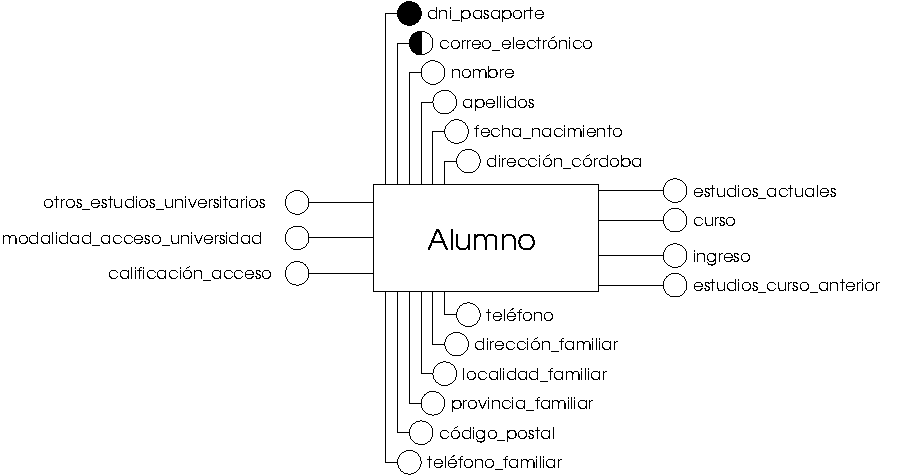
\includegraphics[]{07.Modelo_Entidad-Interrelacion/7.2.Analisis_Entidades/diagramas/alumno.pdf}
            \caption{Diagrama de la entidad Alumno.}
            \label{diagramaAlumno}
            \end{center}
         \end{figure}

   \item[Descripción de los atributos] La entidad presenta los siguientes
   atributos:

   \begin{itemize}
   \item \textbf{dni\_pasaporte}
      \begin{itemize}
         \item \textbf{Definición:} Coincide con el número de documento nacional
         de identidad o pasaporte del alumno.
         \item \textbf{Dominio:} Conjunto de caracteres alfanuméricos.
         \item \textbf{Carácter:} Obligatorio.
         \item \textbf{Ejemplo práctico:} 01234567A.
         \item \textbf{Información adicional:} El dato lo proporciona el usuario alumno, bien a la hora de registrarse, o bien cuando cuando modifica su información personal. Es la clave primaria.
      \end{itemize}
   \item \textbf{correo\_electrónico}
      \begin{itemize}
         \item \textbf{Definición:} Contiene la dirección de correo electrónico de la persona.
         \item \textbf{Dominio:} Conjunto de caracteres alfanuméricos permitidos en una dirección de correo electrónico.
         \item \textbf{Carácter:} Obligatorio.
         \item \textbf{Ejemplo práctico:} i42sasab@uco.es
         \item \textbf{Información adicional:} El dato lo proporciona el usuario alumno cuando se registra o cuando modifica su información personal. Es la clave alterna.
      \end{itemize}
   \item \textbf{nombre}
      \begin{itemize}
         \item \textbf{Definición:} Designa el nombre de pila del usuario alumno que interviene en el sistema.
         \item \textbf{Dominio:} Conjunto de caracteres alfanuméricos.
         \item \textbf{Carácter:} Obligatorio.
         \item \textbf{Ejemplo práctico:} Bartolomé.
         \item \textbf{Información adicional:} El dato lo proporciona el usuario alumno cuando se registra o cuando modifica su información personal.
      \end{itemize}
   \item \textbf{apellidos}
      \begin{itemize}
         \item \textbf{Definición:} Hace referencia a los apellidos del usuario alumno que interviene en el sistema.
         \item \textbf{Dominio:} Conjunto de caracteres alfanuméricos.
         \item \textbf{Carácter:}  Obligatorio.
         \item \textbf{Ejemplo práctico:} Sánchez Salado.
         \item \textbf{Información adicional:} El dato lo proporciona el usuario alumno cuando se registra o cuando modifica su información personal.
      \end{itemize}
   \item \textbf{fecha\_nacimiento}
      \begin{itemize}
         \item \textbf{Definición:} Contiene la fecha de nacimiento del alumno.
         \item \textbf{Dominio:} Formato de fecha: dd-mm-aaaa.
         \item \textbf{Carácter:}  Opcional.
         \item \textbf{Ejemplo práctico:} 13-12-1984.
         \item \textbf{Información adicional:} El dato lo proporciona el usuario alumno cuando se registra o cuando modifica su información personal.
      \end{itemize}
   \item \textbf{dirección\_córdoba}
      \begin{itemize}
         \item \textbf{Definición:} Hace referencia a la dirección del alumno durante el curso.
         \item \textbf{Dominio:} Conjunto de caracteres alfanuméricos.
         \item \textbf{Carácter:}  Opcional.
         \item \textbf{Ejemplo práctico:} 13 Rue del Percebe.
         \item \textbf{Información adicional:} El dato lo proporciona el usuario alumno cuando se registra o cuando modifica su información personal.
      \end{itemize}
   \item \textbf{teléfono}
      \begin{itemize}
         \item \textbf{Definición:} Hace referencia a un número de teléfono perteneciente al alumno.
         \item \textbf{Dominio:} Conjunto de enteros positivos.
         \item \textbf{Carácter:}  Opcional.
         \item \textbf{Ejemplo práctico:} 601234567.
         \item \textbf{Información adicional:} El dato lo proporciona el usuario alumno cuando se registra o cuando modifica su información personal.
      \end{itemize}
   \item \textbf{dirección\_familiar}
      \begin{itemize}
         \item \textbf{Definición:} Hace referencia a la dirección del domicilio familiar del alumno.
         \item \textbf{Dominio:} Conjunto de caracteres alfanuméricos.
         \item \textbf{Carácter:}  Opcional.
         \item \textbf{Ejemplo práctico:} Calle Edsger Dijkstra, 30.
         \item \textbf{Información adicional:} El dato lo proporciona el usuario alumno cuando se registra o cuando modifica su información personal.
      \end{itemize}
   \item \textbf{localidad\_familiar}
      \begin{itemize}
         \item \textbf{Definición:} Hace referencia a la localidad del domicilio familiar del alumno.
         \item \textbf{Dominio:} Conjunto de caracteres alfanuméricos.
         \item \textbf{Carácter:}  Opcional.
         \item \textbf{Ejemplo práctico:} La Carlota.
         \item \textbf{Información adicional:} El dato lo proporciona el usuario alumno cuando se registra o cuando modifica su información personal.
      \end{itemize}
   \item \textbf{provincia\_familiar}
      \begin{itemize}
         \item \textbf{Definición:} Hace referencia a la provincia del domicilio familiar del alumno.
         \item \textbf{Dominio:} Conjunto de caracteres alfanuméricos.
         \item \textbf{Carácter:}  Opcional.
         \item \textbf{Ejemplo práctico:} Córdoba.
         \item \textbf{Información adicional:} El dato lo proporciona el usuario alumno cuando se registra o cuando modifica su información personal.
      \end{itemize}
   \item \textbf{código\_postal}
      \begin{itemize}
         \item \textbf{Definición:} Hace referencia al código postal de la localidad del domicilio familiar del alumno.
         \item \textbf{Dominio:} Conjunto de caracteres alfanuméricos.
         \item \textbf{Carácter:}  Opcional.
         \item \textbf{Ejemplo práctico:} 14100.
         \item \textbf{Información adicional:} El dato lo proporciona el usuario alumno cuando se registra o cuando modifica su información personal.
      \end{itemize}
   \item \textbf{teléfono\_familiar}
      \begin{itemize}
         \item \textbf{Definición:} Hace referencia al número de teléfono del domicilio familiar del alumno.
         \item \textbf{Dominio:} Conjunto de enteros positivos.
         \item \textbf{Carácter:}  Opcional.
         \item \textbf{Ejemplo práctico:} 957123456.
         \item \textbf{Información adicional:} El dato lo proporciona el usuario alumno cuando se registra o cuando modifica su información personal.
      \end{itemize}
   \item \textbf{ingreso}
      \begin{itemize}
         \item \textbf{Definición:} Hace referencia al año de ingreso en la Universidad por parte del alumno en sus estudios actuales.
         \item \textbf{Dominio:} Formato de fecha: aaaa.
         \item \textbf{Carácter:}  Opcional.
         \item \textbf{Ejemplo práctico:} 2004.
         \item \textbf{Información adicional:} El dato lo proporciona el usuario alumno cuando se registra o cuando modifica su información personal.
      \end{itemize}
   \item \textbf{otros\_estudios\_universitarios}
      \begin{itemize}
         \item \textbf{Definición:} Hace referencia a otros estudios universitarios que posea el alumno.
         \item \textbf{Dominio:} Conjunto de caracteres alfanuméricos.
         \item \textbf{Carácter:}  Opcional.
         \item \textbf{Ejemplo práctico:} -
         \item \textbf{Información adicional:} El dato lo proporciona el usuario alumno cuando se registra o cuando modifica su información personal. Se trata de un atributo múltiple.
      \end{itemize}
   \item \textbf{modalidad\_acceso\_universidad}
      \begin{itemize}
         \item \textbf{Definición:} Hace referencia al modo en que el alumno accedió a la Universidad.
         \item \textbf{Dominio:} Conjunto de caracteres alfanuméricos.
         \item \textbf{Carácter:}  Opcional.
         \item \textbf{Ejemplo práctico:} Selectividad.
         \item \textbf{Información adicional:} El dato lo proporciona el usuario alumno cuando se registra o cuando modifica su información personal.
      \end{itemize}
   \item \textbf{calificación\_acceso}
      \begin{itemize}
         \item \textbf{Definición:} Hace referencia a la calificación obtenida en las distintas modalidades de acceso a la Universidad por parte del alumno.
         \item \textbf{Dominio:} Conjunto de reales positivos.
         \item \textbf{Carácter:}  Opcional.
         \item \textbf{Ejemplo práctico:} 7.2.
         \item \textbf{Información adicional:} El dato lo proporciona el usuario alumno cuando se registra o cuando modifica su información personal.
      \end{itemize}
   \end{itemize}

   \item[Ejemplo práctico]

   \item \begin{center}
            \begin{tabular}{ | l | l | }
            \hline
            \multicolumn{2}{ | c | }{\textbf{Tipo de entidad Alumno}} \\
            \hline
            dni\_pasaporte & 01234567A \\
            \hline
            correo\_electrónico & i42sasab@uco.es\\
            \hline
            nombre & Bartolomé\\
            \hline
            apellidos & Sánchez Salado\\
            \hline
            fecha\_nacimiento & 1984\\
            \hline
            dirección\_córdoba & 13 Rue del Percebe\\
            \hline
            teléfono & 601234567\\
            \hline
            dirección\_familiar & Calle Edsger Dijkstra, 30\\
            \hline
            localidad\_familiar & La Carlota\\
            \hline
            provincia\_familiar & Córdoba\\
            \hline
            código\_postal & 14100\\
            \hline
            teléfono\_familiar & 957123456\\
            \hline
            ingreso & 2004\\
            \hline
            otros\_estudios\_universitarios & -\\
            \hline
            modalidad\_acceso\_universidad & Selectividad\\
            \hline
            calificación\_acceso & 7.2\\
            \hline
            \end{tabular}
         \end{center}
   \end{description}

   \subsection{Tipo de entidad Asesor}

   \begin{description}

   \item[Definición] Se refiere a la persona del mundo real: \emph{``Tutor que
        realiza un seguimiento permanente y orientado a la optimización del
        esfuerzo de estudio de un alumno en un curso académico''}.

   \item[Características] La entidad presenta las siguientes características:
      \begin{itemize}
         \item \textbf{Nombre:} Asesor.
         \item \textbf{Tipo:} Fuerte.
         \item \textbf{Número de atributos:} 4.
         \item \textbf{Atributo/s identificador/es principal/es:} dni\_pasaporte.
         \item \textbf{Atributo/s identificador/es alternativo/s:} correo\_electronico.
         \item \textbf{Atributo/s heredado/s:} -
      \end{itemize}

   \item[Diagrama] La figura \ref{diagramaAsesor} muestra el diagrama de la entidad.
   \item \begin{figure}[!ht]
            \begin{center}
            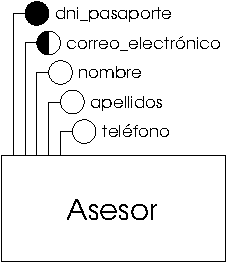
\includegraphics[]{07.Modelo_Entidad-Interrelacion/7.2.Analisis_Entidades/diagramas/asesor.pdf}
            \caption{Diagrama de la entidad Asesor.}
            \label{diagramaAsesor}
            \end{center}
         \end{figure}

   \item[Descripción de los atributos] La entidad presenta los siguientes
   atributos:

   \begin{itemize}
   \item \textbf{dni\_pasaporte}
      \begin{itemize}
         \item \textbf{Definición:} Coincide con el documento nacional de identidad o pasaporte de la persona.
         \item \textbf{Dominio:} Conjunto de caracteres alfanuméricos.
         \item \textbf{Carácter:} Obligatorio.
         \item \textbf{Ejemplo práctico:} 98765432Z.
         \item \textbf{Información adicional:} El dato lo proporciona el administrador, principal o de centro, cuando introduce al usuario asesor en el sistema. Es la clave primaria.
      \end{itemize}
   \item \textbf{correo\_electrónico}
      \begin{itemize}
         \item \textbf{Definición:} Contiene la dirección de correo electrónico de la persona.
         \item \textbf{Dominio:} Conjunto de caracteres alfanuméricos permitidos en una dirección de correo electrónico.
         \item \textbf{Carácter:} Opcional.
         \item \textbf{Ejemplo práctico:} ma1fegan@uco.es
         \item \textbf{Información adicional:} El dato lo proporciona o bien el usuario administrador, principal o de centro, cuando registra al asesor en el sistema, o bien el propio usuario asesor cuando modifica su información personal. Es la clave alterna.
      \end{itemize}
   \item \textbf{nombre}
      \begin{itemize}
         \item \textbf{Definición:} Designa el nombre de pila del usuario asesor que interviene en el sistema.
         \item \textbf{Dominio:} Conjunto de caracteres alfanuméricos.
         \item \textbf{Carácter:} Obligatorio.
         \item \textbf{Ejemplo práctico:} Nicolás Luis.
         \item \textbf{Información adicional:} El dato lo proporciona o bien el usuario administrador, principal o de centro, cuando registra al asesor en el sistema, o bien el propio usuario asesor cuando modifica su información personal.
      \end{itemize}
   \item \textbf{apellidos}
      \begin{itemize}
         \item \textbf{Definición:} Hace referencia a los apellidos del usuario asesor que interviene en el sistema.
         \item \textbf{Dominio:} Conjunto de caracteres alfanuméricos.
         \item \textbf{Carácter:}  Opcional.
         \item \textbf{Ejemplo práctico:} Fernández García.
         \item \textbf{Información adicional:} El dato lo proporciona o bien el usuario administrador, principal o de centro, cuando registra al asesor en el sistema, o bien el propio usuario asesor cuando modifica su información personal.
      \end{itemize}
   \end{itemize}

   \item[Ejemplo práctico]

   \item \begin{center}
            \begin{tabular}{ | l | l | }
            \hline
            \multicolumn{2}{ | c | }{\textbf{Tipo de entidad Asesor}} \\
            \hline
            dni\_pasaporte & 98765432Z \\
            \hline
            correo\_electrónico & ma1fegan@uco.es\\
            \hline
            nombre & Nicolás Luis\\
            \hline
            apellidos & Fernández García\\
            \hline
            \end{tabular}
         \end{center}
   \end{description}

   \subsection{Tipo de entidad Administrador Centro}

   \begin{description}

   \item[Definición] Se refiere al objeto del mundo real: \emph{``Individuo que
    gestiona la información relativa a un centro''}.

   \item[Características] La entidad presenta las siguientes características:
      \begin{itemize}
         \item \textbf{Nombre:} Administrador Centro.
         \item \textbf{Tipo:} Débil por existencia con respecto a Centro.
         \item \textbf{Número de atributos:} 2.
         \item \textbf{Atributo/s identificador/es principal/es:} id\_centro.
         \item \textbf{Atributo/s identificador/es alternativo/s:} -
         \item \textbf{Atributo/s heredado/s:} nombre\_centro, del tipo de
               entidad Centro.
      \end{itemize}

   \item[Diagrama]
   \item \begin{figure}[h!]
            \begin{center}
            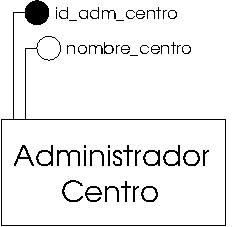
\includegraphics[]{07.Modelo_Entidad-Interrelacion/7.2.Analisis_Entidades/diagramas/adm_centro.pdf}
            \caption{Diagrama de la entidad Administrador Centro}
            \end{center}
         \end{figure}

   \item[Descripción de los atributos] La entidad presenta los siguientes
   atributos:

   \begin{itemize}
    \item \textbf{id\_adm\_centro}
      \begin{itemize}
         \item \textbf{Definición:} Código que sirve como número identificativo
               para cada usuario administrador de centro del sistema.
         \item \textbf{Dominio:} Números naturales.
         \item \textbf{Carácter:} Obligatorio.
         \item \textbf{Ejemplo práctico:} 9.
         \item \textbf{Información adicional:} El dato lo genera el sistema
               cuando el administrador principal introduce un nuevo usuario
               administrador de centro. Es la clave primaria.
      \end{itemize}
   \item \textbf{nombre\_centro}
      \begin{itemize}
         \item \textbf{Definición:} Denominación de un centro dentro del sistema.
         \item \textbf{Dominio:} Conjunto de caracteres alfanuméricos.
         \item \textbf{Carácter:} Obligatorio.
         \item \textbf{Ejemplo práctico:} Escuela Politécnica Superior.
         \item \textbf{Información adicional:} El dato se hereda de la entidad
               Centro.
      \end{itemize}
   \end{itemize}

   \item[Ejemplo práctico]

   \item \begin{center}
            \begin{tabular}{ | l | l | }
            \hline
            \multicolumn{2}{ | c | }{\textbf{Tipo de entidad Administrador Centro}} \\
            \hline
            id\_adm\_centro & 9 \\
            \hline
            nombre\_centro & Escuela Politécnica Superior \\
            \hline
            \end{tabular}
         \end{center}
   \end{description}

   \subsection{Tipo de entidad Centro}

   \begin{description}

   \item[Definición] Se refiere al objeto del mundo real: \emph{``Institución académica de la Universidad de Córdoba donde se imparten títulos universitarios''}.

   \item[Características] La entidad presenta las siguientes características:
      \begin{itemize}
         \item \textbf{Nombre:} Centro.
         \item \textbf{Tipo:} Fuerte.
         \item \textbf{Número de atributos:} 2.
         \item \textbf{Atributo/s identificador/es principal/es:} id\_centro.
         \item \textbf{Atributo/s identificador/es alternativo/s:} nombre\_centro.
         \item \textbf{Atributo/s heredado/s:} -
      \end{itemize}

   \item[Diagrama] La figura \ref{diagramaCentro} muestra el diagrama de la entidad.
   \item \begin{figure}[!ht]
            \begin{center}
            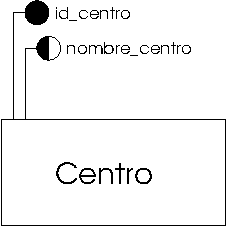
\includegraphics[]{07.Modelo_Entidad-Interrelacion/7.2.Analisis_Entidades/diagramas/centro.pdf}
            \caption{Diagrama de la entidad Centro.}
            \label{diagramaCentro}
            \end{center}
         \end{figure}

   \item[Descripción de los atributos] La entidad presenta los siguientes
   atributos:

   \begin{itemize}
    \item \textbf{id\_centro}
      \begin{itemize}
         \item \textbf{Definición:} Código que sirve como número identificativo
               para cada centro del sistema.
         \item \textbf{Dominio:} Números naturales.
         \item \textbf{Carácter:} Obligatorio.
         \item \textbf{Ejemplo práctico:} 15.
         \item \textbf{Información adicional:} El dato lo genera el sistema
               cuando el administrador principal introduce un nuevo centro en
               el sistema. Es la clave primaria.
      \end{itemize}
   \item \textbf{nombre\_centro}
      \begin{itemize}
         \item \textbf{Definición:} Denominación de un centro dentro del sistema.
         \item \textbf{Dominio:} Conjunto de caracteres alfanuméricos.
         \item \textbf{Carácter:} Obligatorio.
         \item \textbf{Ejemplo práctico:} Escuela Politécnica Superior.
         \item \textbf{Información adicional:} El dato lo introduce el
         administrador principal al introducir un nuevo centro en el sistema. Es
         clave alterna.
      \end{itemize}
   \end{itemize}

   \item[Ejemplo práctico]

   \item \begin{center}
            \begin{tabular}{ | l | l | }
            \hline
            \multicolumn{2}{ | c | }{\textbf{Tipo de entidad Centro}} \\
            \hline
            id\_centro & 15 \\
            \hline
            nombre\_centro & Escuela Politécnica Superior \\
            \hline
            \end{tabular}
         \end{center}
   \end{description}

   \subsection{Tipo de entidad Departamento}

   \begin{description}

   \item[Definición] Se refiere al objeto del mundo real: \emph{``Unidad
   estructural universitaria de docencia e investigación, formada por una o
   varias cátedras de materias afines''}.

   \item[Características] La entidad presenta las siguientes características:
      \begin{itemize}
         \item \textbf{Nombre:} Departamento.
         \item \textbf{Tipo:} Fuerte.
         \item \textbf{Número de atributos:} 2.
         \item \textbf{Atributo/s identificador/es principal/es:} id\_departamento.
         \item \textbf{Atributo/s identificador/es alternativo/s:} nombre\_departamento.
         \item \textbf{Atributo/s heredado/s:} -
      \end{itemize}

   \item[Diagrama] La figura \ref{diagramaDepartamento} muestra el diagrama de la entidad.
   \item \begin{figure}[!ht]
            \begin{center}
            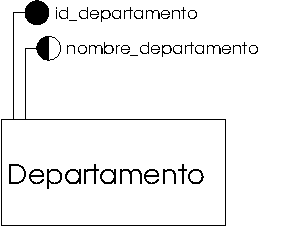
\includegraphics[]{07.Modelo_Entidad-Interrelacion/7.2.Analisis_Entidades/diagramas/departamento.pdf}
            \caption{Diagrama de la entidad Departamento.}
            \label{diagramaDepartamento}
            \end{center}
         \end{figure}

   \item[Descripción de los atributos] La entidad presenta los siguientes
   atributos:

   \begin{itemize}
    \item \textbf{id\_departamento}
      \begin{itemize}
         \item \textbf{Definición:} Código que sirve como número identificativo
               para cada departamento del sistema.
         \item \textbf{Dominio:} Números naturales.
         \item \textbf{Carácter:} Obligatorio.
         \item \textbf{Ejemplo práctico:} 22.
         \item \textbf{Información adicional:} El dato lo genera el sistema
               cuando el administrador principal introduce un nuevo departamento
               en el sistema. Es la clave primaria.
      \end{itemize}
   \item \textbf{nombre\_departamento}
      \begin{itemize}
         \item \textbf{Definición:} Denominación de un departamento dentro del sistema.
         \item \textbf{Dominio:} Conjunto de caracteres alfanuméricos.
         \item \textbf{Carácter:} Obligatorio.
         \item \textbf{Ejemplo práctico:} Departamento de Informática y Análisis Numérico.
         \item \textbf{Información adicional:} El dato lo introduce el
         administrador principal al introducir un nuevo departamento en el sistema. Es
         clave alterna.
      \end{itemize}
   \end{itemize}

   \item[Ejemplo práctico]

   \item \begin{center}
            \begin{tabular}{ | l | l | }
            \hline
            \multicolumn{2}{ | c | }{\textbf{Tipo de entidad Departamento}} \\
            \hline
            id\_departamento & 22 \\
            \hline
            nombre\_departamento & Departamento de Informática y Análisis Numérico \\
            \hline
            \end{tabular}
         \end{center}
   \end{description}

   \subsection{Tipo de entidad Titulación}

   \begin{description}

   \item[Definición] Se refiere al objeto del mundo real: \emph{``Conjunto de
        materias cuya superación supone la obtención de un título académico''}.

   \item[Características] La entidad presenta las siguientes características:
      \begin{itemize}
         \item \textbf{Nombre:} Titulación.
         \item \textbf{Tipo:} Fuerte.
         \item \textbf{Número de atributos:} 2.
         \item \textbf{Atributo/s identificador/es principal/es:} id\_titulacion.
         \item \textbf{Atributo/s identificador/es alternativo/s:} nombre\_titulacion
         \item \textbf{Atributo/s heredado/s:} -
      \end{itemize}

   \item[Diagrama]
   \item \begin{figure}[h!]
            \begin{center}
            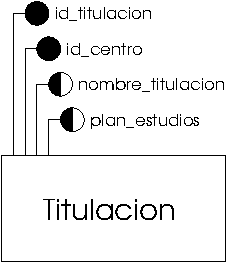
\includegraphics[]{07.Modelo_Entidad-Interrelacion/7.2.Analisis_Entidades/diagramas/titulacion.pdf}
            \caption{Diagrama de la entidad Titulación}
            \end{center}
         \end{figure}

   \item[Descripción de los atributos] La entidad presenta los siguientes
   atributos:

   \begin{itemize}
    \item \textbf{id\_titulacion}
      \begin{itemize}
         \item \textbf{Definición:} Código que sirve como número identificativo
         para cada titulación dentro del sistema.
         \item \textbf{Dominio:} Números naturales.
         \item \textbf{Carácter:} Obligatorio.
         \item \textbf{Ejemplo práctico:} 3.
         \item \textbf{Información adicional:} El dato lo genera el sistema
         cuando el administrador introduce la titulación en el sistema.
         Es la clave primaria.
      \end{itemize}
   \item \textbf{nombre\_titulacion}
      \begin{itemize}
         \item \textbf{Definición:} Denominación de una titulación dentro del sistema.
         \item \textbf{Dominio:} Conjunto de caracteres alfanuméricos.
         \item \textbf{Carácter:} Obligatorio.
         \item \textbf{Ejemplo práctico:} Ingeniería Técnica en Informática de Gestión.
         \item \textbf{Información adicional:} El dato lo proporciona el administrador en el momento de introducir la titulación en el sistema. Es la clave alterna
      \end{itemize}
   \end{itemize}

   \item[Ejemplo práctico]

   \item \begin{center}
            \begin{tabular}{ | l | l | }
            \hline
            \multicolumn{2}{ | c | }{\textbf{Tipo de entidad Titulación}} \\
            \hline
            id\_centro & 3 \\
            \hline
            nombre\_centro & Ingeniería Técnica en Informática de Gestión \\
            \hline
            \end{tabular}
         \end{center}
   \end{description}

   \subsection{Tipo de entidad Asignatura}

   \begin{description}

   \item[Definición] Se refiere al objeto del mundo real: \emph{``Materia que
   forma parte del plan de estudios de una titulación''}.

   \item[Características] La entidad presenta las siguientes características:
      \begin{itemize}
         \item \textbf{Nombre:} Asignatura.
         \item \textbf{Tipo:} Débil por identificación con respecto a Titulación.
         \item \textbf{Número de atributos:} 8.
         \item \textbf{Atributo/s identificador/es principal/es:} id\_centro junto con \\id\_titulación e id\_asignatura.
         \item \textbf{Atributo/s identificador/es alternativo/s:} id\_centro junto con \\id\_titulación y nombre\_asignatura.
         \item \textbf{Atributo/s heredado/s:} id\_centro del tipo de entidad Centro, \\id\_titulación del tipo de entidad Titulación.
      \end{itemize}

   \item[Diagrama] La figura \ref{diagramaAsignatura} muestra el diagrama de la entidad.
   \item \begin{figure}[!ht]
            \begin{center}
            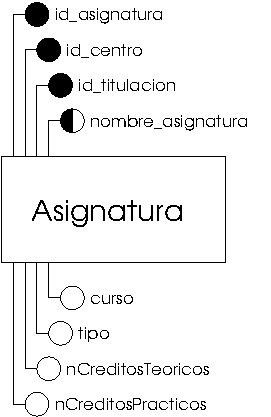
\includegraphics[]{07.Modelo_Entidad-Interrelacion/7.2.Analisis_Entidades/diagramas/asignatura.pdf}
            \caption{Diagrama de la entidad Asignatura.}
            \label{diagramaAsignatura}
            \end{center}
         \end{figure}

   \item[Descripción de los atributos] La entidad presenta los siguientes
   atributos:

   \begin{itemize}
   \item \textbf{id\_centro}
      \begin{itemize}
         \item \textbf{Definición:} Código que sirve como número identificativo
               para cada centro del sistema.
         \item \textbf{Dominio:} Números naturales.
         \item \textbf{Carácter:} Obligatorio.
         \item \textbf{Ejemplo práctico:} 15.
         \item \textbf{Información adicional:} El dato se hereda del tipo de
         entidad Centro. Es la clave primaria junto con id\_titulación e
         id\_asignatura. También actúa de clave alterna junto con
         id\_titulación y nombre\_asignatura.
      \end{itemize}
   \item \textbf{id\_titulación}
      \begin{itemize}
         \item \textbf{Definición:} Código que sirve como número identificativo
         para cada titulación dentro del sistema.
         \item \textbf{Dominio:} Números naturales.
         \item \textbf{Carácter:} Obligatorio.
         \item \textbf{Ejemplo práctico:} 3.
         \item \textbf{Información adicional:} El dato se hereda del tipo de
         entidad Titulación. Es la clave primaria junto con id\_centro e
         id\_asignatura. También actúa de clave alterna junto con
         id\_centro y nombre\_asignatura.
      \end{itemize}
   \item \textbf{id\_asignatura}
      \begin{itemize}
         \item \textbf{Definición:} Código que sirve como número identificativo
         para cada asignatura dentro del sistema.
         \item \textbf{Dominio:} Números naturales.
         \item \textbf{Carácter:} Obligatorio.
         \item \textbf{Ejemplo práctico:} 17.
         \item \textbf{Información adicional:} El dato lo proporciona el sistema, cuando el administrador, principal o de centro, introduce la asignatura en el sistema. Es la clave primaria junto con id\_centro y con id\_titulación.
      \end{itemize}
   \item \textbf{nombre\_asignatura}
      \begin{itemize}
         \item \textbf{Definición:} Denominación de una asignatura dentro del sistema.
         \item \textbf{Dominio:} Conjunto de caracteres alfanuméricos.
         \item \textbf{Carácter:}  Obligatorio.
         \item \textbf{Ejemplo práctico:} Lenguajes de Inteligencia Artificial.
         \item \textbf{Información adicional:} El dato lo proporciona el administrador, principal o de
         centro, en el momento de introducir la asignatura en el sistema. Es la clave alterna junto con
         id\_centro y con id\_titulación.
      \end{itemize}
   \item \textbf{curso}
      \begin{itemize}
         \item \textbf{Definición:} Nivel académico de la asignatura en una titulación.
         \item \textbf{Dominio:} Números naturales.
         \item \textbf{Carácter:}  Opcional.
         \item \textbf{Ejemplo práctico:} 2.
         \item \textbf{Información adicional:} El dato lo proporciona el administrador, principal o de
         centro, en el momento de introducir la asignatura en el sistema.
      \end{itemize}
   \item \textbf{tipo}
      \begin{itemize}
         \item \textbf{Definición:} Clasificación de la asignatura según su tipo.
         \item \textbf{Dominio:} Uno de los valores: Troncal, Obligatoria, Optativa o Libre Configuración.
         \item \textbf{Carácter:}  Opcional.
         \item \textbf{Ejemplo práctico:} Optativa.
         \item \textbf{Información adicional:} El dato lo proporciona el administrador, principal o de
         centro, en el momento de introducir la asignatura en el sistema.
      \end{itemize}
   \item \textbf{nCréditosTeóricos}
      \begin{itemize}
         \item \textbf{Definición:} Valor relacionado con el número de horas que se estima necesario para dedicar al contenido teórico de una asignatura.
         \item \textbf{Dominio:} Números reales positivos.
         \item \textbf{Carácter:}  Opcional.
         \item \textbf{Ejemplo práctico:} 3.0.
         \item \textbf{Información adicional:} El dato lo proporciona el administrador, principal o de
         centro, en el momento de introducir la asignatura en el sistema.
      \end{itemize}
   \item \textbf{nCréditosPrácticos}
      \begin{itemize}
         \item \textbf{Definición:} Valor relacionado con el número de horas que se estima necesario para dedicar al contenido práctico de una asignatura.
         \item \textbf{Dominio:} Números reales positivos.
         \item \textbf{Carácter:}  Opcional.
         \item \textbf{Ejemplo práctico:} 1.5.
         \item \textbf{Información adicional:} El dato lo proporciona el administrador, principal o de
         centro, en el momento de introducir la asignatura en el sistema.
      \end{itemize}

   \end{itemize}

   \item[Ejemplo práctico]

   \item \begin{center}
            \begin{tabular}{ | l | l | }
            \hline
            \multicolumn{2}{ | c | }{\textbf{Tipo de entidad Asignatura}} \\
            \hline
            id\_centro & 15 \\
            \hline
            id\_titulación & 3\\
            \hline
            id\_asignatura & 17\\
            \hline
            nombre\_asignatura & Lenguajes de Inteligencia Artificial\\
            \hline
            curso & 2\\
            \hline
            tipo & Optativa\\
            \hline
            nCréditosTeóricos & 3.0\\
            \hline
            nCréditosPrácticos & 1.5\\
            \hline
            \end{tabular}
         \end{center}
   \end{description}

   \subsection{Tipo de entidad Asignatura Curso Académico}

   \begin{description}

   \item[Definición] Se refiere al objeto del mundo real: \emph{``Asignatura
   impartida en un determinado curso académico''}.

   \item[Características] La entidad presenta las siguientes características:
      \begin{itemize}
         \item \textbf{Nombre:} Asignatura Curso Académico.
         \item \textbf{Tipo:} Débil por identificación con respecto a Asignatura.
         \item \textbf{Número de atributos:} 1 propio y 3 heredados.
         \item \textbf{Atributo/s identificador/es principal/es:} id\_centro junto con \\id\_titulación, id\_asignatura y curso\_académico.
         \item \textbf{Atributo/s identificador/es alternativo/s:} -
         \item \textbf{Atributo/s heredado/s:} id\_centro, id\_titulación e
         id\_asignatura del tipo de entidad Asignatura.
      \end{itemize}

   \item[Diagrama] La figura \ref{diagramaACA} muestra el diagrama de la entidad.
   \item \begin{figure}[!ht]
            \begin{center}
            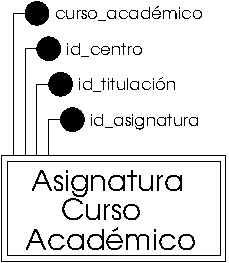
\includegraphics[]{07.Modelo_Entidad-Interrelacion/7.2.Analisis_Entidades/diagramas/aca.pdf}
            \caption{Diagrama de la entidad Asignatura Curso Académico.}
            \label{diagramaACA}
            \end{center}
         \end{figure}

   \item[Descripción de los atributos propios] La entidad presenta los
   siguientes atributos propios:

   \begin{itemize}
   \item \textbf{curso\_académico}
      \begin{itemize}
         \item \textbf{Definición:} Hace referencia al periodo de tiempo en que se imparte una determinada asignatura.
         \item \textbf{Dominio:} Formato de fecha: aaaa.
         \item \textbf{Carácter:}  Obligatorio.
         \item \textbf{Ejemplo práctico:} 2008.
         \item \textbf{Información adicional:} El dato lo proporciona el usuario alumno al establecer las asignaturas en las cuales se ha matriculado. Es la clave primaria junto con id\_centro, id\_titulación e id\_asignatura.
      \end{itemize}
   \end{itemize}

   \item[Ejemplo práctico]

   \item \begin{center}
            \begin{tabular}{ | l | l | }
            \hline
            \multicolumn{2}{ | c | }{\textbf{Tipo de entidad Asignatura Curso Académico}} \\
            \hline
            id\_centro & 15 \\
            \hline
            id\_titulación & 3\\
            \hline
            id\_asignatura & 17\\
            \hline
            curso\_académico & 2008\\
            \hline
            \end{tabular}
         \end{center}
   \end{description}

   \subsection{Tipo de entidad Alumno Curso Académico}

   \begin{description}

   \item[Definición] Se refiere al objeto del mundo real: \emph{``Estudiante de
   una titulación matriculado durante un curso académico''}.

   \item[Características] La entidad presenta las siguientes características:
      \begin{itemize}
         \item \textbf{Nombre:} Alumno Curso Académico.
         \item \textbf{Tipo:} Débil por identificación con respecto a Alumno.
         \item \textbf{Número de atributos:} 2 propios y 1 heredado.
         \item \textbf{Atributo/s identificador/es principal/es:} dni\_pasaporte y \\curso\_académico.
         \item \textbf{Atributo/s identificador/es alternativo/s:} -
         \item \textbf{Atributo/s heredado/s:} dni\_pasaporte del tipo
         de entidad Alumno.
      \end{itemize}

   \item[Diagrama] La figura \ref{diagramaAlumnoCA} muestra el diagrama de la entidad.
   \item \begin{figure}[!ht]
            \begin{center}
            
\includegraphics[]{07.Modelo_Entidad-Interrelacion/7.2.Analisis_Entidades/diagramas/alumnoca.pdf}
            \caption{Diagrama de la entidad Alumno Curso Académico.}
            \label{diagramaAlumnoCA}
            \end{center}
         \end{figure}

   \item[Descripción de los atributos propios] Esta entidad presenta el
   siguiente atributo propio:

   \begin{itemize}
   \item \textbf{curso\_académico}
      \begin{itemize}
         \item \textbf{Definición:} Hace referencia al periodo de tiempo en que se imparte una determinada asignatura.
         \item \textbf{Dominio:} Formato de fecha: aaaa.
         \item \textbf{Carácter:}  Obligatorio.
         \item \textbf{Ejemplo práctico:} 2008.
         \item \textbf{Información adicional:} El dato representa el primer año
         del curso académico. Es la clave primaria junto con dni\_pasaporte.
      \end{itemize}
   \item \textbf{observaciones}
      \begin{itemize}
         \item \textbf{Definición:} Información extra que pueda ser necesario
         conocer.
         \item \textbf{Dominio:} Conjunto de caracteres alfanuméricos.
         \item \textbf{Carácter:}  Opcional.
         \item \textbf{Ejemplo práctico:} Tiene beca.
         \item \textbf{Información adicional:} El dato lo proporicona el usuario
         alumno al modificar su información personal.
      \end{itemize}
   \end{itemize}

   \item[Ejemplo práctico]

   \item \begin{center}
            \begin{tabular}{ | l | l | }
            \hline
            \multicolumn{2}{ | c | }{\textbf{Tipo de entidad Alumno Curso Académico}} \\
            \hline
            dni\_pasaporte & 01234567A \\
            \hline
            curso\_académico & 2008 \\
            \hline
            observaciones & Tiene beca \\
            \hline
            \end{tabular}
         \end{center}
   \end{description}

   \subsection{Tipo de entidad Asesor Curso Académico}

   \begin{description}

   \item[Definición] Se refiere al objeto del mundo real: \emph{``Asesor
   que realiza labor de tutoría durante un curso académico''}.

   \item[Características] La entidad presenta las siguientes características:
      \begin{itemize}
         \item \textbf{Nombre:} Asesor Curso Académico.
         \item \textbf{Tipo:} Débil por identificación con respecto a Asesor y débil por existencia respecto a Departamento.
         \item \textbf{Número de atributos:} 1 propio y 1 heredado.
         \item \textbf{Atributo/s identificador/es principal/es:} dni\_pasaporte y \\curso\_académico.
         \item \textbf{Atributo/s identificador/es alternativo/s:} -
         \item \textbf{Atributo/s heredado/s:} dni\_pasaporte del tipo
         de entidad Asesor.
      \end{itemize}

   \item[Diagrama] La figura \ref{diagramaAsesorCA} muestra el diagrama de la entidad.
   \item \begin{figure}[!ht]
            \begin{center}
            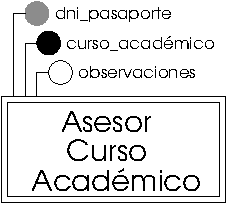
\includegraphics[]{07.Modelo_Entidad-Interrelacion/7.2.Analisis_Entidades/diagramas/asesorca.pdf}
            \caption{Diagrama de la entidad Asesor Curso Académico.}
            \label{diagramaAsesorCA}
            \end{center}
         \end{figure}

   \item[Descripción de los atributos propios] Esta entidad presenta el
   siguiente atributo propio:

   \begin{itemize}
   \item \textbf{curso\_académico}
      \begin{itemize}
         \item \textbf{Definición:} Hace referencia al periodo de tiempo en que se imparte una determinada asignatura.
         \item \textbf{Dominio:} Formato de fecha: aaaa.
         \item \textbf{Carácter:}  Obligatorio.
         \item \textbf{Ejemplo práctico:} 2007.
         \item \textbf{Información adicional:} El dato \textit{¿quién lo proporciona?}. Es la clave primaria junto con dni\_pasaporte.
      \end{itemize}
   \end{itemize}

   \item[Ejemplo práctico]

   \item \begin{center}
            \begin{tabular}{ | l | l | }
            \hline
            \multicolumn{2}{ | c | }{\textbf{Tipo de entidad Asesor Curso Académico}} \\
            \hline
            dni\_pasaporte & 98765432Z \\
            \hline
            curso\_académico & 2007\\
            \hline
            \end{tabular}
         \end{center}
   \end{description}

      \section{Análisis de interrelaciones}

   \paragraph{}Una vez definidas las distintas entidades presentes en el
   modelo, a continuación se detallarán las distintas relaciones que mantienen
   entre ellas. Las interrelaciones por describir son las siguientes:

   \begin{itemize}
    \item Interrelación Administrador Centro - Centro.
    \item Interrelación Centro - Titulación.
    \item Interrelación Titulación - Asignatura.
    \item Interrelación Asignatura - Asignatura Curso Académico.
    \item Interrelación Alumno - Alumno Curso Académico.
    \item Interrelación Alumno Curso Académico - Matrícula.
    \item Interrelación Asignatura Curso Académico - Matrícula.
    \item Interrelación Asesor - Asesor Curso Académico.
    \item Interrelación Departamento - Asesor Curso Académico.
    \item Interrelación Asesor Curso Académico - Plantilla Entrevista Asesor.
    \item Interrelación Plantilla Entrevista Asesor - Pregunta Asesor.
    \item Interrelación Asesor Curso Académico - Alumno Curso Académico.
    \item Interrelación Plantilla Entrevista Oficial - Pregunta Oficial.
    \item Interrelación Alumno Curso Académico - Reunión.
    \item Interrelación Reunión - Pregunta Oficial.
    \item Interrelación Reunión - Pregunta Asesor.
   \end{itemize}

   \paragraph{}Para la descripción de cada relación entre entidades, se
   utilizarán los siguientes apartados:

   \begin{description}
      \item[Definición] Especifica el motivo por el cual se produce la
           interrelación y entre qué tipos de entidad se da lugar.

      \item[Características] En este aparatado se mostrará la siguiente
           información:

            \begin{itemize}
             \item Nombre del tipo de interrelación.
             \item Tipo de la interrelación, es decir, fuerte o débil. En el
                   caso de que sea débil se especifica el tipo de debilidad:
                   existencia o identificación.
             \item Cardinalidad de la interrelación y cardinalidad con la que
                   cada tipo de entidad participa en la interrelación.
             \item Número de atributos del tipo de interrelación.
             \item Posibles restricciones que pueda tener la interrelación, en
                   el caso de que hubiera.
            \end{itemize}

      \item[Diagrama] Representación gráfica del tipo de interrelación.

      \item[Descripción de los atributos] Se describirán cada uno de los
           atributos que forman parte del tipo de interrelación. Para cada uno
           de ellos se indicará lo siguiente:

           \begin{itemize}
            \item Definición del atributo.
            \item Dominio en el cual se encuentra.
            \item Ejemplo práctico de cada atributo.
           \end{itemize}

      \item[Ejemplo práctico del tipo de interrelación] En este apartado se
           muestra una ocurrencia concreta del tipo de interrelación.
   \end{description}

\subsection{Interrelación Administrador Centro - Centro}

   \begin{description}
      \item[Definición] En esta interrelación se deja constancia de que cada
      centro establecido en el sistema dispone, al menos, un administrador de
      centro.

      \item[Características] La interrelación presenta las siguientes
                             características:

         \begin{itemize}
            \item \textbf{Nombre:} AC-C
            \item \textbf{Tipo de la interrelación:} Fuerte
            \item \textbf{Cardinalidad de la interrelación:} N:M
                  \begin{itemize}
                     \item Administrador Centro: administra (0,n)
                     \item Centro: es\_administrado\_por (1,n)
                  \end{itemize}
            \item \textbf{Número de atributos:} Ninguno
         \end{itemize}

      \item[Diagrama] La figura \ref{diagramaAC-C} muestra el diagrama de la
                      interrelación.
      \item \begin{figure}[!ht]
            \begin{center}
            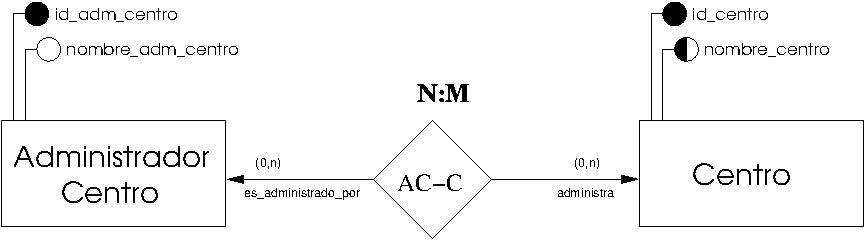
\includegraphics[]{07.Modelo_Entidad-Interrelacion/7.3.Analisis_Interrelaciones/diagramas/AC-C.pdf}
            \caption{Diagrama de la interrelación AC-C.}
            \label{diagramaAC-C}
            \end{center}
         \end{figure}

      \item[Ejemplo práctico del tipo de interrelación]

      \item \begin{center}
            \begin{tabular}{ | c | c | }
            \hline
            \multicolumn{2}{ | c | }{\textbf{Tipo de interrelación AC-C}} \\
            \hline
            \textbf{Administrador Centro} & \textbf{Centro}\\
            \hline
            id\_adm\_centro & id\_centro \\
            \hline
            9 & 15 \\
            \hline
            \end{tabular}
         \end{center}

   \end{description}

\subsection{Interrelación Centro - Titulación}

   \begin{description}
      \item[Definición]

      \item[Características] La interrelación presenta las siguientes
                             características:

         \begin{itemize}
            \item \textbf{Nombre:}
            \item \textbf{Tipo de la interrelación:}
            \item \textbf{Cardinalidad de la interrelación:}
            \item \textbf{Número de atributos:}
         \end{itemize}

      \item[Diagrama] La figura \textit{RELLENAR} muestra el diagrama de la
                      interrelación.

      \item[Descripción de los atributos]

      \item[Ejemplo práctico del tipo de interrelación]
   \end{description}

\subsection{Interrelación Titulación - Asignatura}

   \begin{description}
      \item[Definición] En esta interrelación se deja constancia de que cada
      titulación establecida en el sistema podrá disponer de varias asignaturas.

      \begin{itemize}
       \item Una titulación puede disponer de varias asignaturas.
       \item Una asignatura solamente puede pertenecer a una determinada
             titulación.
      \end{itemize}

      \item[Características] La interrelación presenta las siguientes
                             características:

         \begin{itemize}
            \item \textbf{Nombre:} T-A
            \item \textbf{Tipo de la interrelación:} El tipo de entidad
                  Asignatura es débil por identificación respecto al tipo de
                  entidad Titulación.
            \item \textbf{Cardinalidad de la interrelación:} 1:N
                  \begin{itemize}
                     \item Titulación: dispone\_de (0,n)
                     \item Asignatura: pertenece\_a (1,1)
                  \end{itemize}
            \item \textbf{Número de atributos:} Ninguno.
         \end{itemize}

      \item[Diagrama] La figura \ref{diagramaT-A} muestra el diagrama de la
                      interrelación.

      \item \begin{figure}[!ht]
            \begin{center}
            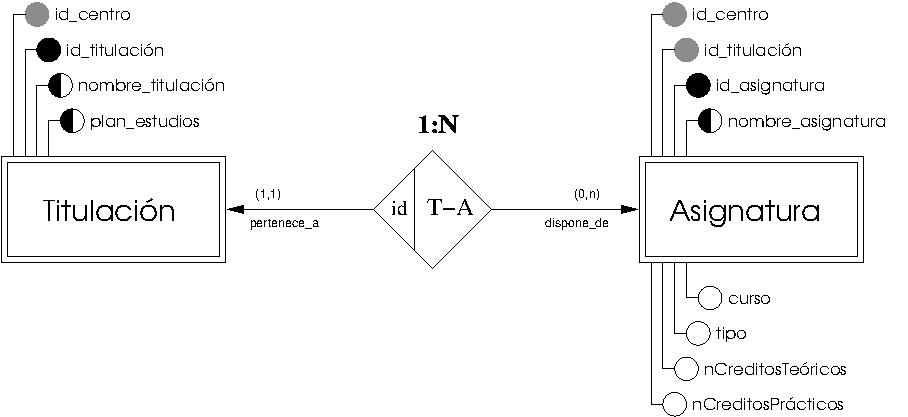
\includegraphics[]{07.Modelo_Entidad-Interrelacion/7.3.Analisis_Interrelaciones/diagramas/T-A.pdf}
            \caption{Diagrama de la interrelación T-A.}
            \label{diagramaT-A}
            \end{center}
         \end{figure}

      \item[Ejemplo práctico del tipo de interrelación]

      \item \begin{center}
            \begin{tabular}{ | r r | }
            \hline
            \multicolumn{2}{ | c | }{\textbf{Tipo de interrelación T-A}} \\
            \hline
            \textbf{Titulación} & \\
            id\_centro & 15 \\
            id\_titulación & 3 \\
            \hline
            \textbf{Asignatura} & \\
            id\_centro & 15 \\
            id\_titulación & 3 \\
            id\_asignatura & 17 \\
            \hline
            \end{tabular}
         \end{center}
   \end{description}

\subsection{Interrelación Asignatura - Asignatura Curso Académico}

   \begin{description}
      \item[Definición]

      \item[Características] La interrelación presenta las siguientes
                             características:

         \begin{itemize}
            \item \textbf{Nombre:}
            \item \textbf{Tipo de la interrelación:}
            \item \textbf{Cardinalidad de la interrelación:}
            \item \textbf{Número de atributos:}
         \end{itemize}

      \item[Diagrama] La figura \textit{RELLENAR} muestra el diagrama de la
                      interrelación.

      \item[Descripción de los atributos]

      \item[Ejemplo práctico del tipo de interrelación]
   \end{description}

\subsection{Interrelación Alumno - Alumno Curso Académico}

   \begin{description}
      \item[Definición] En esta interrelación se deja constancia de que un
      alumno puede estar matriculado durante un número indeterminado de cursos
      académicos.

      \item[Características] La interrelación presenta las siguientes
                             características:

         \begin{itemize}
            \item \textbf{Nombre:} A-AlCA
            \item \textbf{Tipo de la interrelación:} El tipo de entidad
                  Alumno Curso Académico es débil por identificación respecto al
                  tipo de entidad Alumno.
            \item \textbf{Cardinalidad de la interrelación:} 1:N
                  \begin{itemize}
                     \item Alumno: matriculado\_en (0,n)
                     \item Alumno Curso Académico: es\_un (1,1)
                  \end{itemize}
            \item \textbf{Número de atributos:} Ninguno.
         \end{itemize}

      \item[Diagrama] La figura \ref{diagramaA-AlCA} muestra el diagrama de la
                      interrelación.

      \item \begin{figure}[!ht]
            \begin{center}
            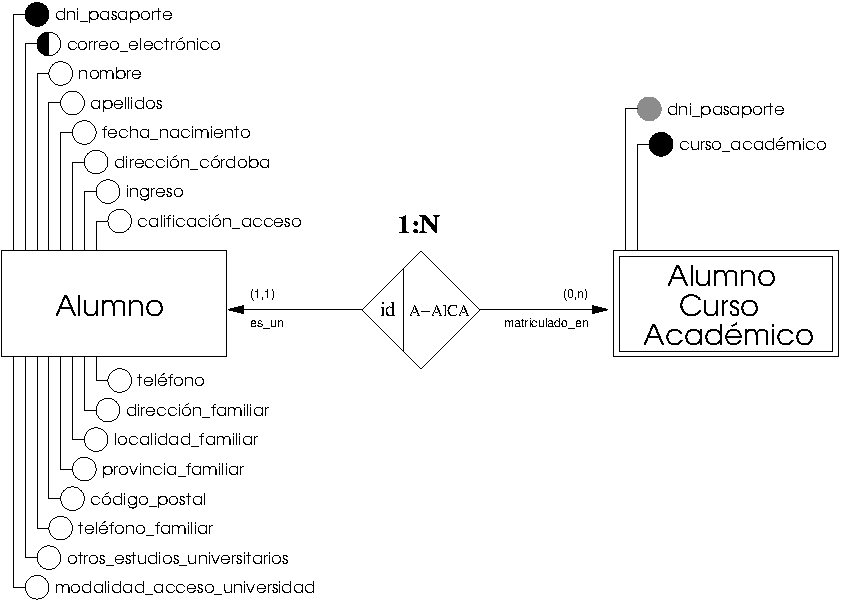
\includegraphics[]{07.Modelo_Entidad-Interrelacion/7.3.Analisis_Interrelaciones/diagramas/A-AlCA.pdf}
            \caption{Diagrama de la interrelación A-AlCA.}
            \label{diagramaA-AlCA}
            \end{center}
         \end{figure}

      \item[Ejemplo práctico del tipo de interrelación]

      \item \begin{center}
            \begin{tabular}{ | r r | }
            \hline
            \multicolumn{2}{ | c | }{\textbf{Tipo de interrelación A-AlCA}} \\
            \hline
            \textbf{Alumno} & \\
            dni\_pasaporte & 01234567A \\
            \hline
            \textbf{Alumno Curso Académico} & \\
            dni\_pasaporte & 01234567A \\
            curso\_académico & 2008 \\
            \hline
            \end{tabular}
         \end{center}
   \end{description}

\subsection{Interrelación Alumno Curso Académico - Matrícula}

   \begin{description}
      \item[Definición] En esta interrelación se deja constancia de que un
      alumno estará matriculado de una determinada asignatura durante un curso
      académico.

      \begin{itemize}
       \item Un \textit{Alumno Curso Académico} puede tener varias
             \textit{Matrícula}.
       \item Una \textit{Matrícula} solamente puede pertenecer a un
             \textit{Alumno Curso Académico}.
      \end{itemize}

      \item[Características] La interrelación presenta las siguientes
                             características:

         \begin{itemize}
            \item \textbf{Nombre:} AlCA-M
            \item \textbf{Tipo de la interrelación:} El tipo de entidad
                  Matrícula es débil por identificación respecto al tipo de
                  entidad Alumno Curso Académico.
            \item \textbf{Cardinalidad de la interrelación:} 1:N
                  \begin{itemize}
                     \item Alumno Curso Académico: tiene (0,n)
                     \item Matrícula: pertenece\_a (1,1)
                  \end{itemize}
            \item \textbf{Número de atributos:} Ninguno.
         \end{itemize}

      \item[Diagrama] La figura \ref{diagramaAlCA-M} muestra el diagrama de la
                      interrelación.

      \item \begin{figure}[!ht]
            \begin{center}
            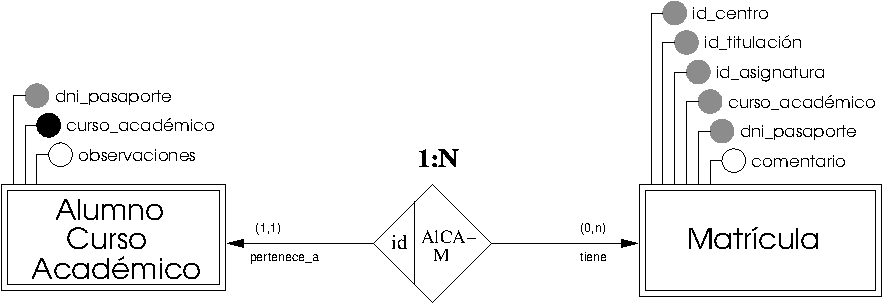
\includegraphics[]{07.Modelo_Entidad-Interrelacion/7.3.Analisis_Interrelaciones/diagramas/AlCA-M.pdf}
            \caption{Diagrama de la interrelación AlCA-M.}
            \label{diagramaAlCA-M}
            \end{center}
         \end{figure}

      \item[Ejemplo práctico del tipo de interrelación]

      \item \begin{center}
            \begin{tabular}{ | r r | }
            \hline
            \multicolumn{2}{ | c | }{\textbf{Tipo de interrelación AlCA-M}} \\
            \hline
            \textbf{Alumno Curso Académico} & \\
            dni\_pasaporte & 01234567A \\
            curso\_académico & 2008 \\
            \hline
            \textbf{Matrícula} & \\
            id\_centro & 15 \\
            id\_titulación & 3\\
            id\_asignatura & 17\\
            curso\_académico & 2008 \\
            dni\_pasaporte & 01234567A \\
            \hline
            \end{tabular}
         \end{center}
   \end{description}

\subsection{Interrelación Asignatura Curso Académico - Matrícula}

   \begin{description}
      \item[Definición] En esta interrelación se deja constancia de que es
      posible realizar una matrícula de una determinada asignatura durante un
      curso académico.

      \begin{itemize}
       \item Una \textit{Asignatura Curso Académico} puede tener varias
             \textit{Matrícula}.
       \item Una \textit{Matrícula} solamente puede
             pertenecer a una \textit{Asignatura Curso \newline Académico}.
      \end{itemize}

      \item[Características] La interrelación presenta las siguientes
                             características:

         \begin{itemize}
            \item \textbf{Nombre:} ACA-M
            \item \textbf{Tipo de la interrelación:} El tipo de entidad
                  Matrícula es débil por identificación
                  respecto al tipo de entidad Alumno Curso Académico.
            \item \textbf{Cardinalidad de la interrelación:} 1:N
                  \begin{itemize}
                     \item Asignatura Curso Académico: tiene (0,n)
                     \item Matrícula: pertenece\_a (1,1)
                  \end{itemize}
            \item \textbf{Número de atributos:} Ninguno.
         \end{itemize}

      \item[Diagrama] La figura \ref{diagramaACA-M} muestra el diagrama de la
                      interrelación.

      \item \begin{figure}[!ht]
            \begin{center}
            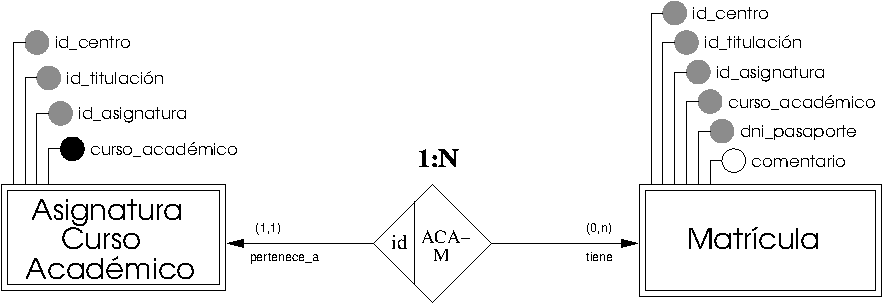
\includegraphics[]{07.Modelo_Entidad-Interrelacion/7.3.Analisis_Interrelaciones/diagramas/ACA-M.pdf}
            \caption{Diagrama de la interrelación ACA-M.}
            \label{diagramaACA-M}
            \end{center}
         \end{figure}

      \item[Ejemplo práctico del tipo de interrelación]

      \item \begin{center}
            \begin{tabular}{ | r r | }
            \hline
            \multicolumn{2}{ | c | }{\textbf{Tipo de interrelación ACA-M}} \\
            \hline
            \textbf{Asignatura Curso Académico} & \\
            id\_centro & 15 \\
            id\_titulación & 3\\
            id\_asignatura & 17\\
            curso\_académico & 2008\\
            \hline
            \textbf{Matrícula} & \\
            id\_centro & 15 \\
            id\_titulación & 3\\
            id\_asignatura & 17\\
            curso\_académico & 2008 \\
            dni\_pasaporte & 01234567A \\
            \hline
            \end{tabular}
         \end{center}
   \end{description}

\subsection{Interrelación Asesor - Asesor Curso Académico}

   \begin{description}
      \item[Definición] En esta interrelación se deja constancia de que un
      asesor puede ofrecer servicios de asesoría durante distintos cursos
      académicos.

      \begin{itemize}
       \item Un \textit{Asesor} puede asesorar a varios \textit{Asesor Curso Académico}.
       \item Un \textit{Asesor Curso Académico} es un \textit{Asesor}.
      \end{itemize}

      \item[Características] La interrelación presenta las siguientes
                             características:

         \begin{itemize}
            \item \textbf{Nombre:} Ase-AseCA
            \item \textbf{Tipo de la interrelación:} El tipo de entidad
                  Asesor Curso Académico es débil por identificación respecto al
                  tipo de entidad Asesor.
            \item \textbf{Cardinalidad de la interrelación:} 1:N
                  \begin{itemize}
                     \item Asesor: asesora (0,n)
                     \item Asesor Curso Académico: es\_un (1,1)
                  \end{itemize}
            \item \textbf{Número de atributos:} Ninguno.
         \end{itemize}

      \item[Diagrama] La figura \ref{diagramaAse-AseCA} muestra el diagrama de la
                      interrelación.

      \item \begin{figure}[!ht]
            \begin{center}
            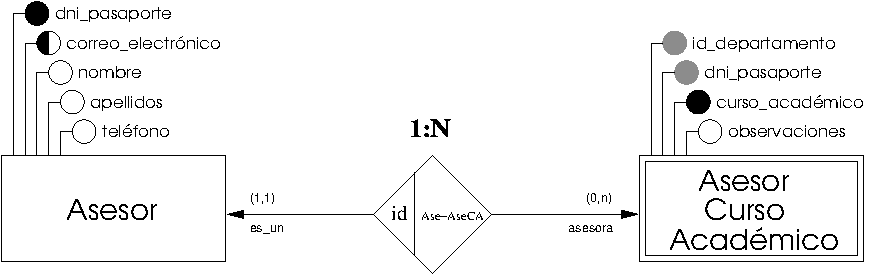
\includegraphics[]{07.Modelo_Entidad-Interrelacion/7.3.Analisis_Interrelaciones/diagramas/Ase-AseCA.pdf}
            \caption{Diagrama de la interrelación Ase-AseCA.}
            \label{diagramaAse-AseCA}
            \end{center}
         \end{figure}

      \item[Ejemplo práctico del tipo de interrelación]

      \item \begin{center}
            \begin{tabular}{ | r r | }
            \hline
            \multicolumn{2}{ | c | }{\textbf{Tipo de interrelación Ase-AseCA}} \\
            \hline
            \textbf{Asesor} & \\
            dni\_pasaporte & 98765432Z \\
            \hline
            \textbf{Asesor Curso Académico} & \\
            dni\_pasaporte & 98765432Z \\
            id\_centro & 2008 \\
            \hline
            \end{tabular}
         \end{center}
   \end{description}

\subsection{Interrelación Departamento - Asesor Curso Académico}

   \begin{description}
      \item[Definición] En esta interrelación se deja constancia de que un
      asesor puede ofrecer servicios de asesoría perteneciendo a un departamento
      durante un determinado curso académico.

      \item[Características] La interrelación presenta las siguientes
                             características:

         \begin{itemize}
            \item \textbf{Nombre:} D-AseCA
            \item \textbf{Tipo de la interrelación:} El tipo de entidad
                  Asesor Curso Académico es débil por existencia respecto al
                  tipo de entidad Departamento.
            \item \textbf{Cardinalidad de la interrelación:} 1:N
            \item \textbf{Número de atributos:} Ninguno.
         \end{itemize}

      \item[Diagrama] La figura \ref{diagramaD-AseCA} muestra el diagrama de la
                      interrelación.

      \item \begin{figure}[!ht]
            \begin{center}
            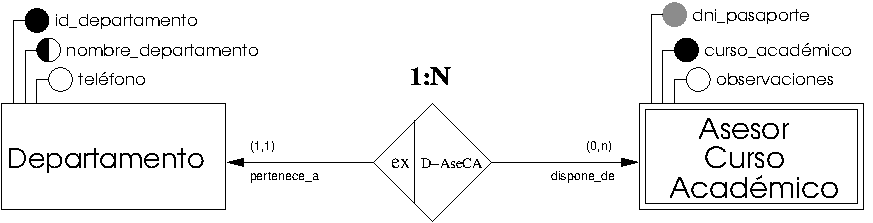
\includegraphics[]{07.Modelo_Entidad-Interrelacion/7.3.Analisis_Interrelaciones/diagramas/D-AseCA.pdf}
            \caption{Diagrama de la interrelación D-AseCA.}
            \label{diagramaD-AseCA}
            \end{center}
         \end{figure}

      \item[Ejemplo práctico del tipo de interrelación]

      \item \begin{center}
            \begin{tabular}{ | r r | }
            \hline
            \multicolumn{2}{ | c | }{\textbf{Tipo de interrelación D-AseCA}} \\
            \hline
            \textbf{Departamento} & \\
            id\_departamento & 22 \\
            \hline
            \textbf{Asesor Curso Académico} & \\
            dni\_pasaporte & 98765432Z \\
            curso\_académico & 2007 \\
            \hline
            \end{tabular}
         \end{center}
   \end{description}

\subsection{Interrelación Plantilla Entrevista Asesor - Asesor Curso Académico}

   \begin{description}
      \item[Definición] En esta interrelación se deja constancia de que un
      usuario asesor puede hacer uso de plantillas de entrevistas de asesor
      durante un determinado curso académico.

      \item[Características] La interrelación presenta las siguientes
                             características:

         \begin{itemize}
            \item \textbf{Nombre:} AseCA-PEA
            \item \textbf{Tipo de la interrelación:} El tipo de entidad
            Plantilla Entrevista Asesor es débil por identificación respecto al
            tipo de entidad Asesor Curso Académico.
            \item \textbf{Cardinalidad de la interrelación:} 1:N
                  \begin{itemize}
                     \item Asesor Curso Académico: utiliza (0,n)
                     \item Plantilla Entrevista Asesor: utilizada\_por (1,1)
                  \end{itemize}
            \item \textbf{Número de atributos:} Ninguno.
         \end{itemize}

      \item[Diagrama] La figura \ref{diagramaPEA-AseCA} muestra el diagrama de
      la interrelación.

      \item \begin{figure}[!ht]
            \begin{center}
            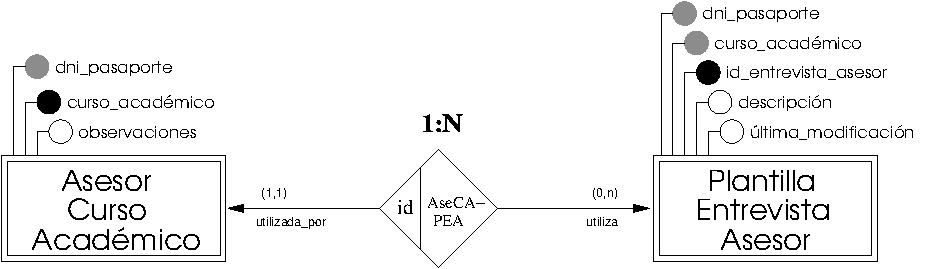
\includegraphics[]{07.Modelo_Entidad-Interrelacion/7.3.Analisis_Interrelaciones/diagramas/PEA-AseCA.pdf}
            \caption{Diagrama de la interrelación PEA-AseCA.}
            \label{diagramaPEA-AseCA}
            \end{center}
         \end{figure}

      \item[Ejemplo práctico del tipo de interrelación]

      \item \begin{center}
            \begin{tabular}{ | r r | }
            \hline
            \multicolumn{2}{ | c | }{\textbf{Tipo de interrelación AseCA-PEA}} \\
            \hline
            \textbf{Asesor Curso Académico} & \\
            dni\_pasaporte & 98765432Z \\
            curso\_académico & 2008 \\
            \hline
            \textbf{Plantilla Entrevista Asesor} & \\
            dni\_pasaporte & 98765432Z \\
            curso\_académico & 2008 \\
            id\_entrevista\_asesor & 36 \\
            \hline
            \end{tabular}
         \end{center}
   \end{description}

\subsection{Interrelación Plantilla Entrevista Asesor - Pregunta Asesor}

   \begin{description}
      \item[Definición] En esta interrelación se deja constancia de que una
      plantilla de entrevista de asesor puede estar compuesta por varias
      preguntas de asesor.

      \item[Características] La interrelación presenta las siguientes
                             características:

         \begin{itemize}
            \item \textbf{Nombre:} PEA-PA
            \item \textbf{Tipo de la interrelación:} El tipo de entidad Pregunta
                  Asesor es débil por identificación respecto al tipo de
                  entidad Plantilla Entrevista Asesor.
            \item \textbf{Cardinalidad de la interrelación:} 1:N
                  \begin{itemize}
                     \item Plantilla Entrevista Asesor: contiene (0,n)
                     \item Pregunta Asesor: forma\_parte\_de (1,1)
                  \end{itemize}
            \item \textbf{Número de atributos:} Ninguno.
         \end{itemize}

      \item[Diagrama] La figura \ref{diagramaPEA-PA} muestra el diagrama de la
                      interrelación.

      \item \begin{figure}[!ht]
            \begin{center}
            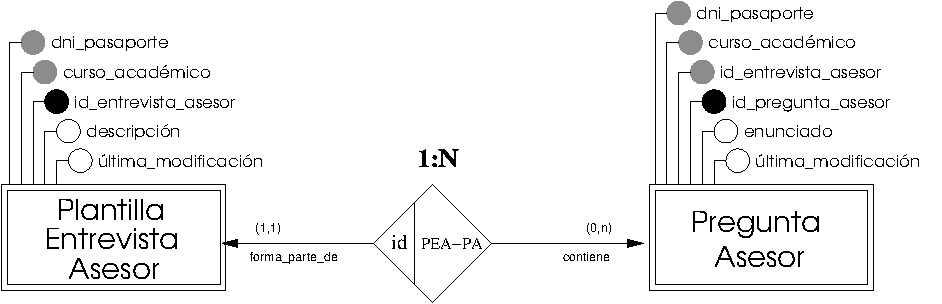
\includegraphics[]{07.Modelo_Entidad-Interrelacion/7.3.Analisis_Interrelaciones/diagramas/PEA-PA.pdf}
            \caption{Diagrama de la interrelación PEA-PA.}
            \label{diagramaPEA-PA}
            \end{center}
         \end{figure}

      \item[Ejemplo práctico del tipo de interrelación]

      \item \begin{center}
            \begin{tabular}{ | r r | }
            \hline
            \multicolumn{2}{ | c | }{\textbf{Tipo de interrelación PEA-PA}} \\
            \hline
            \textbf{Plantilla Entrevista Asesor} & \\
            dni\_pasaporte & 98765432Z \\
            curso\_académico & 2008 \\
            id\_entrevista\_asesor & 36 \\
            \hline
            \textbf{Pregunta Asesor} & \\
            dni\_pasaporte & 98765432Z \\
            curso\_académico & 2008 \\
            id\_entrevista\_asesor & 36 \\
            id\_pregunta\_asesor & 72 \\
            \hline
            \end{tabular}
         \end{center}
   \end{description}

\subsection{Interrelación Asesor Curso Académico - Alumno Curso Académico}

   \begin{description}
      \item[Definición] En esta interrelación se deja constancia de que un
      asesor puede ofrecer servicios de asesoría a un número indeterminado de
      alumnos matriculados durante un determinado curso académico.

      \item[Características] La interrelación presenta las siguientes
                             características:

         \begin{itemize}
            \item \textbf{Nombre:} AseCA-AlCA
            \item \textbf{Tipo de la interrelación:} El tipo de entidad
                  Alumno Curso Académico es débil por existencia respecto al
                  tipo de entidad Asesor Curso Académico.
            \item \textbf{Cardinalidad de la interrelación:} 1:N
                  \begin{itemize}
                     \item Asesor Curso Académico: asesora\_a (0,n)
                     \item Alumno Curso Académico: es\_asesorado\_por (1,1)
                  \end{itemize}
            \item \textbf{Número de atributos:} Ninguno.
            \item \textbf{Restricciones:} Los atributos
                   \textit{curso\_académico} de cada una de las dos entidades
                   que participan en esta interrelación deben tener el mismo
                   valor, por la propia naturaleza de dicha interrelación.
         \end{itemize}

      \item[Diagrama] La figura \ref{diagramaAseCA-AlCA} muestra el diagrama de
                      la interrelación.

       \item \begin{figure}[!ht]
            \begin{center}
            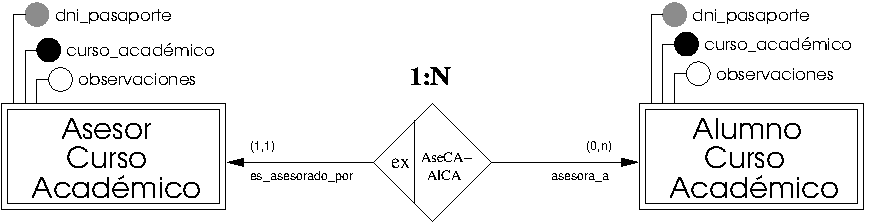
\includegraphics[]{07.Modelo_Entidad-Interrelacion/7.3.Analisis_Interrelaciones/diagramas/AseCA-AlCA.pdf}
            \caption{Diagrama de la interrelación AseCA-AlCA.}
            \label{diagramaAseCA-AlCA}
            \end{center}
         \end{figure}

      \item[Ejemplo práctico del tipo de interrelación]

      \item \begin{center}
            \begin{tabular}{ | r r | }
            \hline
            \multicolumn{2}{ | c | }{\textbf{Tipo de interrelación AseCA-AlCA}} \\
            \hline
            \textbf{Asesor Curso Académico} & \\
            dni\_pasaporte & 98765432Z \\
            curso\_académico & 2008 \\
            \hline
            \textbf{Alumno Curso Académico} & \\
            dni\_pasaporte & 01234567A \\
            curso\_académico & 2008 \\
            \hline
            \end{tabular}
         \end{center}
   \end{description}

\subsection{Interrelación Plantilla Entrevista Oficial - Pregunta Oficial}

   \begin{description}
      \item[Definición] En esta interrelación se deja constancia de que una
      plantilla de entrevista oficial puede estar compuesta por varias preguntas
      oficiales.

      \item[Características] La interrelación presenta las siguientes
                             características:

         \begin{itemize}
            \item \textbf{Nombre:} PEO-PO
            \item \textbf{Tipo de la interrelación:} El tipo de entidad Pregunta
                  Oficial es débil por identificación respecto al tipo de
                  entidad Plantilla Entrevista Oficial.
            \item \textbf{Cardinalidad de la interrelación:} 1:N
                  \begin{itemize}
                     \item Plantilla Entrevista Oficial: contiene (0,n)
                     \item Pregunta Oficial: forma\_parte\_de (1,1)
                  \end{itemize}
            \item \textbf{Número de atributos:} Ninguno.
         \end{itemize}

      \item[Diagrama] La figura \ref{diagramaPEO-PO} muestra el diagrama de la
                      interrelación.

      \item \begin{figure}[!ht]
            \begin{center}
            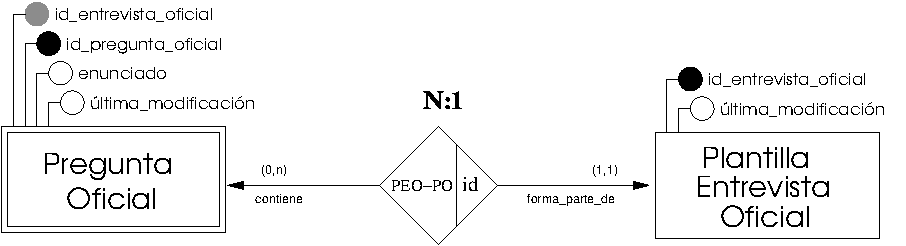
\includegraphics[]{07.Modelo_Entidad-Interrelacion/7.3.Analisis_Interrelaciones/diagramas/PEO-PO.pdf}
            \caption{Diagrama de la interrelación PEO-PO.}
            \label{diagramaPEO-PO}
            \end{center}
         \end{figure}

      \item[Ejemplo práctico del tipo de interrelación]

      \item \begin{center}
            \begin{tabular}{ | r r | }
            \hline
            \multicolumn{2}{ | c | }{\textbf{Tipo de interrelación PEO-PO}} \\
            \hline
            \textbf{Plantilla Entrevista Oficial} & \\
            id\_entrevista\_oficial & 24 \\
            \hline
            \textbf{Pregunta Oficial} & \\
            id\_entrevista\_oficial & 24 \\
            id\_pregunta\_oficial & 55 \\
            \hline
            \end{tabular}
         \end{center}
   \end{description}

\subsection{Interrelación Alumno Curso Académico - Reunión}

   \begin{description}
      \item[Definición] En esta interrelación se deja constancia de que un
      alumno puede participar en reuniones con su asesor durante un determinado
      curso académico.

      \item[Características] La interrelación presenta las siguientes
                             características:

         \begin{itemize}
            \item \textbf{Nombre:} AlCA-R
            \item \textbf{Tipo de la interrelación:} El tipo de entidad Reunión
                  es débil por identificación respecto al tipo de entidad Alumno
                  Curso Académico .
            \item \textbf{Cardinalidad de la interrelación:} 1:N
                  \begin{itemize}
                     \item Alumno Curso Académico: participa\_en (0,n)
                     \item Reunión: realizada\_a (1,1)
                  \end{itemize}
            \item \textbf{Número de atributos:} Ninguno.
         \end{itemize}

      \item[Diagrama] La figura \ref{diagramaAlCA-R} muestra el diagrama de la
                      interrelación.

      \item \begin{figure}[!ht]
            \begin{center}
            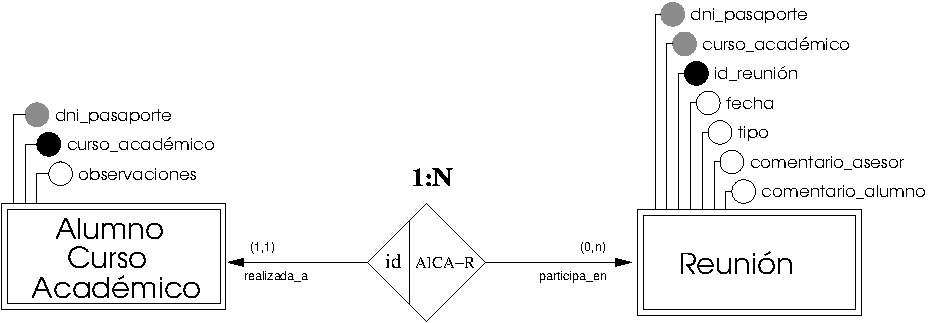
\includegraphics[]{07.Modelo_Entidad-Interrelacion/7.3.Analisis_Interrelaciones/diagramas/AlCA-R.pdf}
            \caption{Diagrama de la interrelación AlCA-R.}
            \label{diagramaAlCA-R}
            \end{center}
         \end{figure}

      \item[Ejemplo práctico del tipo de interrelación]

      \item \begin{center}
            \begin{tabular}{ | r r | }
            \hline
            \multicolumn{2}{ | c | }{\textbf{Tipo de interrelación AlCA-R}} \\
            \hline
            \textbf{Alumno Curso Académico} & \\
            dni\_pasaporte & 01234567A \\
            curso\_académico & 2008 \\
            \hline
            \textbf{Reunión} & \\
            dni\_pasaporte & 98765432Z \\
            curso\_académico & 2008 \\
            id\_reunión & 121 \\
            fecha & 01/01/2009 \\
            tipo & Individual \\
            \hline
            \end{tabular}
         \end{center}
   \end{description}

\subsection{Interrelación Reunión - Pregunta Oficial}

   \begin{description}
      \item[Definición] En esta interrelación se deja constancia de que una
      reunión puede estar compuesta por varias preguntas oficiales.

      \item[Características] La interrelación presenta las siguientes
                             características:

         \begin{itemize}
            \item \textbf{Nombre:} R-PO
            \item \textbf{Tipo de la interrelación:} Fuerte.
            \item \textbf{Cardinalidad de la interrelación:} N:M
                  \begin{itemize}
                     \item Reunión: compuesta\_por (0,n)
                     \item Pregunta Oficial: aparece\_en (0,n)
                  \end{itemize}
            \item \textbf{Número de atributos:} Uno: respuesta.
         \end{itemize}

      \item[Diagrama] La figura \ref{diagramaR-PO} muestra el diagrama de la
                      interrelación.

      \item \begin{figure}[!ht]
            \begin{center}
            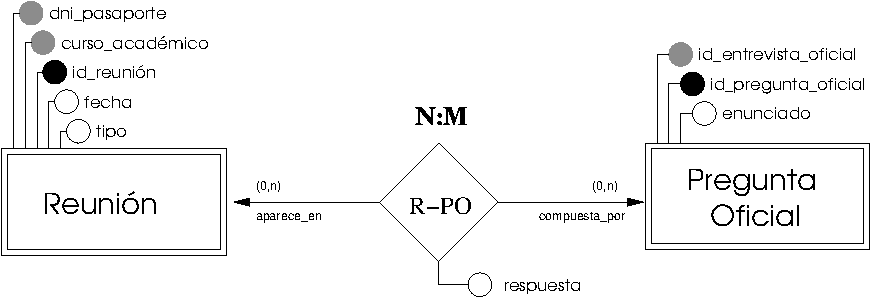
\includegraphics[]{07.Modelo_Entidad-Interrelacion/7.3.Analisis_Interrelaciones/diagramas/R-PO.pdf}
            \caption{Diagrama de la interrelación R-PO.}
            \label{diagramaR-PO}
            \end{center}
         \end{figure}

      \item[Descripción de los atributos] La interrelación presenta el
      siguiente atributo:

       \begin{itemize}
        \item \textbf{respuesta}
          \begin{itemize}
            \item \textbf{Definición:} Establece la contestación del alumno a la
            pregunta realizada.
            \item \textbf{Dominio:} Conjunto de caracteres alfanuméricos.
            \item \textbf{Carácter:} Obligatorio.
            \item \textbf{Ejemplo práctico:} Antiguo alumno.
            \item \textbf{Información adicional:} El dato lo introduce el
            usuario alumno al contestar a la pregunta realizada.
         \end{itemize}
       \end{itemize}

      \item[Ejemplo práctico del tipo de interrelación]

      \item \begin{center}
            \begin{tabular}{ | r r | }
            \hline
            \multicolumn{2}{ | c | }{\textbf{Tipo de interrelación R-PO}} \\
            \hline
            \textbf{Reunión} & \\
            dni\_pasaporte & 98765432Z \\
            curso\_académico & 2008 \\
            id\_reunión & 121 \\
            fecha & 01/01/2009 \\
            tipo & Individual \\
            \hline
            \textbf{Pregunta Oficial} & \\
            id\_entrevista\_oficial & 24 \\
            id\_pregunta\_oficial & 55 \\
            enunciado & ¿Quién le ha informado de esta carrera? \\
            \hline
            \textbf{Atributos} & \\
            respuesta & Antiguo alumno \\
            \hline
            \end{tabular}
         \end{center}
   \end{description}

\subsection{Interrelación Reunión - Pregunta Asesor}

   \begin{description}
      \item[Definición] En esta interrelación se deja constancia de que una
      reunión puede estar compuesta por varias preguntas de asesor.

      \begin{itemize}
       \item Una \textit{Reunión} puede estar compuesta por varias
             \textit{Pregunta Asesor}.
       \item Una \textit{Pregunta Asesor} puede aparecer en varias
             \textit{Reunión}.
      \end{itemize}

      \item[Características] La interrelación presenta las siguientes
                             características:

         \begin{itemize}
            \item \textbf{Nombre:} R-PA
            \item \textbf{Tipo de la interrelación:} Fuerte.
            \item \textbf{Cardinalidad de la interrelación:} N:M
                  \begin{itemize}
                     \item Reunión: compuesta\_por (0,n)
                     \item Pregunta Oficial: aparece\_en (0,n)
                  \end{itemize}
            \item \textbf{Número de atributos:} Uno: respuesta.
            \item \textbf{Restricciones:} Debido a que existe un ciclo en el
                  modelo Entidad-Relación planteado (ver la figura
                  \ref{diagramaER} ) que afecta a las entidades \textit{Alumno
                  Curso Académico}, \textit{Asesor Curso Académico},
                  \textit{Plantilla Entrevista Asesor}, \textit{Pregunta Asesor}
                  y \textit{Reunión}, no es posible controlar que un determinado
                  \textit{Alumno Curso Académico} tenga reuniones exclusivamente
                  con las \textit{Pregunta Asesor} de su \textit{Asesor Curso
                  Académico}, por lo que será necesario controlar este
                  comportamiento mediante la lógica de la aplicación.
         \end{itemize}

      \item[Diagrama] La figura \ref{diagramaR-PA} muestra el diagrama de la
                      interrelación.

      \item \begin{figure}[!ht]
            \begin{center}
            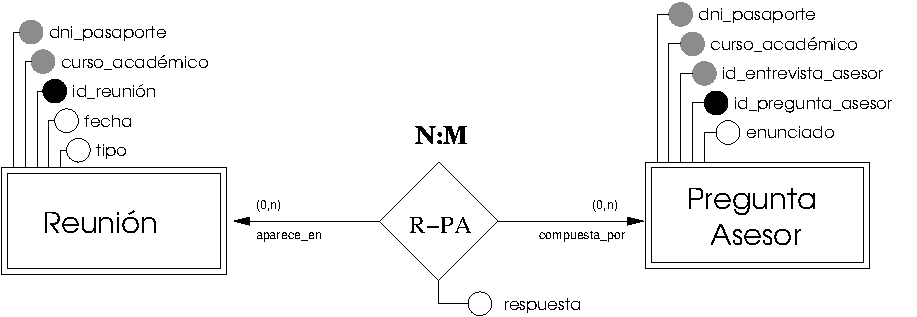
\includegraphics[]{07.Modelo_Entidad-Interrelacion/7.3.Analisis_Interrelaciones/diagramas/R-PA.pdf}
            \caption{Diagrama de la interrelación R-PA.}
            \label{diagramaR-PA}
            \end{center}
         \end{figure}

      \item[Descripción de los atributos] La interrelación presenta el
      siguiente atributo:

       \begin{itemize}
        \item \textbf{respuesta}
          \begin{itemize}
            \item \textbf{Definición:} Establece la contestación del alumno a la
            pregunta realizada.
            \item \textbf{Dominio:} Conjunto de caracteres alfanuméricos.
            \item \textbf{Carácter:} Obligatorio.
            \item \textbf{Ejemplo práctico:} Antiguo alumno.
            \item \textbf{Información adicional:} El dato lo introduce el
            usuario alumno al contestar a la pregunta realizada.
         \end{itemize}
       \end{itemize}

      \item[Ejemplo práctico del tipo de interrelación]

      \item \begin{center}
            \begin{tabular}{ | r r | }
            \hline
            \multicolumn{2}{ | c | }{\textbf{Tipo de interrelación R-PA}} \\
            \hline
            \textbf{Reunión} & \\
            dni\_pasaporte & 98765432Z \\
            curso\_académico & 2008 \\
            id\_reunión & 121 \\
            \hline
            \textbf{Pregunta Asesor} & \\
            dni\_pasaporte & 98765432Z \\
            curso\_académico & 2008 \\
            id\_entrevista\_asesor & 36 \\
            id\_pregunta\_asesor & 72 \\
            enunciado & Nivel de inglés \\
            \hline
            \textbf{Pregunta Asesor} & \\
            respuesta & Alto \\
            \hline
            \end{tabular}
         \end{center}
   \end{description}


      \newpage

\section{Esquema Entidad-Relación}

   \paragraph{}La figura \ref{diagramaER} muestra el diagrama Entidad-Relación.

   \begin{figure}[!ht]
            \begin{center}
            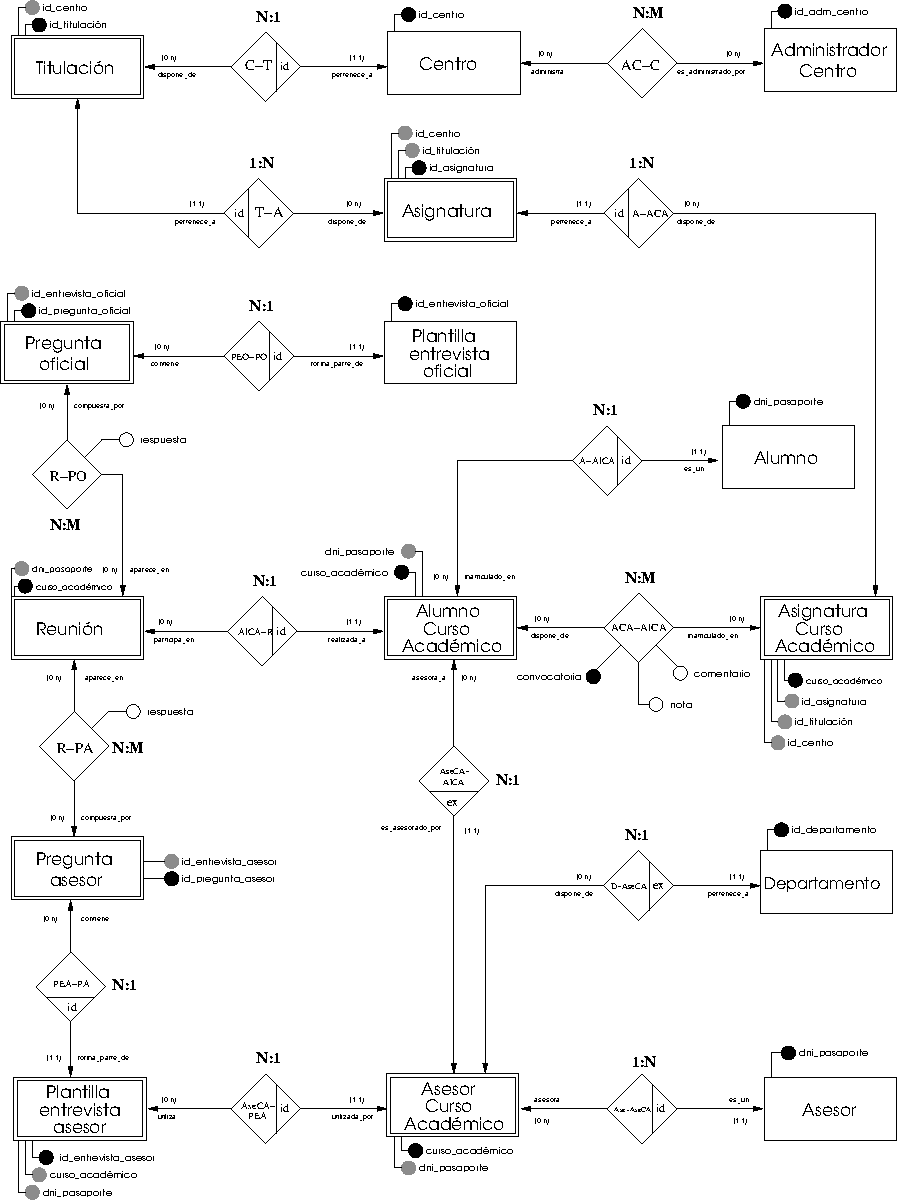
\includegraphics[]{07.Modelo_Entidad-Interrelacion/7.4.Esquema_E-R/diagramaER.pdf}
            \caption{Diagrama Entidad-Relación.}
            \label{diagramaER}
            \end{center}
         \end{figure}

   \chapter{Análisis Funcional}
      \section{Introducción}

  \paragraph{}En este capítulo se muestra una visión detallada del
  comportamiento del sistema de manera que sea entendible tanto por el usuario
  final como por los desarrolladores, mediante una representación de cómo fluye
  la información por el sistema desde su entrada hasta su salida.

  \paragraph{}Para realizar esta representación, se utilizarán una serie de
  Diagramas de Flujo de Datos (DFD) que son una herramienta que permite
  visualizar un sistema como una red de procesos funcionales, conectados entre
  sí por \textit{conductos} y \textit{tanques de almacenamiento} de datos.
  También se utilizará un Diccionario de Datos que realizará una representación
  de los elementos requeridos o producidos por la aplicación.


   \chapter{Especificación de requisitos de la interfaz}\label{espReqInt}

   \chapter{Diseño de datos}
      \section{Introducción}

  \paragraph{}En este capítulo se muestra una visión detallada del
  comportamiento del sistema de manera que sea entendible tanto por el usuario
  final como por los desarrolladores, mediante una representación de cómo fluye
  la información por el sistema desde su entrada hasta su salida.

  \paragraph{}Para realizar esta representación, se utilizarán una serie de
  Diagramas de Flujo de Datos (DFD) que son una herramienta que permite
  visualizar un sistema como una red de procesos funcionales, conectados entre
  sí por \textit{conductos} y \textit{tanques de almacenamiento} de datos.
  También se utilizará un Diccionario de Datos que realizará una representación
  de los elementos requeridos o producidos por la aplicación.

      \section{Modelo de datos relacional}

  \paragraph{}Las tablas obtenidas después de la normalización son las
  siguientes:

  \begin{itemize}
   \item Tabla Centros.
   \item Tabla AdministradoresCentro.
   \item Tabla Titulaciones.
   \item Tabla Asignaturas.
   \item Tabla AsignaturasCursoAcadémico.
   \item Tabla Departamentos.
   \item Tabla Asesores.
   \item Tabla AsesoresCursoAcadémico.
   \item Tabla PlantillasEntrevistaAsesor.
   \item Tabla PreguntasAsesores.
   \item Tabla Alumnos.
   \item Tabla AlumnosCursoAcadémico.
   \item Tabla Matrículas.
   \item Tabla CalificacionesConvocatoria.
   \item Tabla PlantillasEntrevistaOficial.
   \item Tabla PreguntasOficiales.
   \item Tabla Reuniones.
   \item Tabla Centro\_AdministradoresCentro.
   \item Tabla Reunión\_PreguntasAsesor.
   \item Tabla Reunión\_PreguntasOficiales.
  \end{itemize}

   \subsection{Tabla Centros}

      \paragraph{}Esta tabla se obtiene a través del tipo de entidad
      \textit{Centro}, tomando los atributos de ésta (regla
      RTECAR-1\footnote{Según Luque Ruiz et al. \cite{luqueRuiz}, regla
      RTECAR-1: \textit{``Todos los tipos de entidad presentes en el esquema
      conceptual se transformarán en tablas o relaciones en el esquema
      relacional manteniendo el número y tipo de atributos, así como la
      característica de identificador de estos atributos.''}}).

      \paragraph{}La clave principal de esta tabla es el atributo
      \textit{id\_centro}.

      \paragraph{}La tabla \textit{Centros} queda de la siguiente forma:

      \begin{description}
         \item[Centros] \begin{flushleft}(\underline{id\_centro},
         \textsc{nombre\_centro})\end{flushleft}
      \end{description}
\subsection{Tabla AdministradoresCentro}

  \paragraph{}Esta tabla se encuentra en FNBC, ya que cada determinante
  funcional es una clave candidata de la relación.

  \paragraph{}Existen dos dependencias funcionales, la que forma la clave
  primaria de la relación con el resto de atributos y, por otro lado, la que
  forma la clave alterna con el resto de atributos de la relación.

  \begin{center}
    \begin{minipage}{3.7cm}{\begin{flushright}\begin{tabular}{ | c | }
                  \hline
                  id\_adm\_centro \\
                  \hline
                 \end{tabular}\end{flushright} }
    \end{minipage}
    \begin{minipage}{0.7cm}{$\longrightarrow$}
    \end{minipage}
    \begin{minipage}{5.9cm}{\begin{tabular}{ | c | }
                  \hline
                  correo\_electrónico \\
                  nombre\_adm\_centro \\
                  \hline
                 \end{tabular} }
    \end{minipage}
  \end{center}

  \begin{center}
    \begin{minipage}{3.7cm}{\begin{flushright}\begin{tabular}{ | c | }
                  \hline
                  correo\_electrónico \\
                  \hline
                 \end{tabular}\end{flushright} }
    \end{minipage}
    \begin{minipage}{0.7cm}{$\longrightarrow$}
    \end{minipage}
    \begin{minipage}{5.9cm}{\begin{tabular}{ | c | }
                  \hline
                  id\_adm\_centro \\
                  nombre\_adm\_centro \\
                  \hline
                 \end{tabular} }
    \end{minipage}
  \end{center}
   \subsection{Tabla Titulaciones}

      \paragraph{}Esta tabla se obtiene a través del tipo de entidad
      \textit{Titulación}, tomando los atributos de ésta (regla RTECAR-1).
      Además, mantiene una referencia con la tabla \textit{Centro} a través
      del atributo \textit{id\_centro} (regla RTECAR-3.1).

      \paragraph{}La clave principal de la tabla se compone con la agregación de
      los atributos \textit{id\_centro} e \textit{id\_titulación}. Posee una
      clave alterna que será la formada por la agregación de los atributos
      \textit{id\_centro}, \textit{nombre\_titulación} y
      \textit{plan\_estudios}.

      \paragraph{}La tabla \textit{Titulaciones} queda de la siguiente forma:

      \begin{description}
         \item[Titulaciones] \begin{flushleft}(\underline{\textbf{ID\_CENTRO},
         id\_titulación}, \textsc{nombre\_titulación},
         \textsc{plan\_estudios})\end{flushleft}
      \end{description}

\subsection{Tabla Asignaturas}

  \paragraph{}Esta tabla se encuentra en FNBC, ya que cada determinante
  funcional es una clave candidata de la relación.

  \paragraph{}Existen dos dependencias funcionales, la que forma la clave
  primaria de la relación con el resto de atributos y, por otro lado, la que
  forma la clave alterna con el resto de atributos de la relación.

 \begin{center}
    \begin{minipage}{4.2cm}{\begin{flushright}\begin{tabular}{ | c | }
                  \hline
                  (id\_centro + \\
                  id\_titulación + \\
                  id\_asignatura) \\
                  \hline
                 \end{tabular}\end{flushright} }
    \end{minipage}
    \begin{minipage}{0.7cm}{$\longrightarrow$}
    \end{minipage}
    \begin{minipage}{5.9cm}{\begin{tabular}{ | c | }
                  \hline
                  nombre\_asignatura \\
                  curso \\
                  tipo \\
                  nCréditosTeóricos \\
                  nCréditosPrácticos \\
                  \hline
                 \end{tabular} }
    \end{minipage}
  \end{center}

  \begin{center}
    \begin{minipage}{4.2cm}{\begin{tabular}{ | c | }
                  \hline
                  (id\_centro + \\
                  id\_titulación + \\
                  nombre\_asignatura) \\
                  \hline
                 \end{tabular} }
    \end{minipage}
    \begin{minipage}{0.7cm}{$\longrightarrow$}
    \end{minipage}
    \begin{minipage}{5.9cm}{\begin{tabular}{ | c | }
                  \hline
                  id\_asignatura \\
                  curso \\
                  tipo \\
                  nCréditosTeóricos \\
                  nCréditosPrácticos \\
                  \hline
                 \end{tabular} }
    \end{minipage}
  \end{center}

\subsection{Tabla AsignaturasCursoAcadémico}

  \paragraph{}Esta tabla se encuentra en FNBC puesto que el único
  determinante funcional existente es el propio identificador principal
  de la tabla.

 \begin{center}
    \begin{minipage}{4.2cm}{\begin{flushright}\begin{tabular}{ | c | }
                  \hline
                  (id\_centro + \\
                  id\_titulación + \\
                  id\_asignatura + \\
                  curso\_académico) \\
                  \hline
                 \end{tabular}\end{flushright} }
    \end{minipage}
    \begin{minipage}{0.7cm}{$\longrightarrow$}
    \end{minipage}
    \begin{minipage}{5.9cm}{\begin{tabular}{ | c | }
                  \hline
                  \\
                  \hline
                 \end{tabular} }
    \end{minipage}
  \end{center}

   \subsection{Tabla Departamentos}

      \paragraph{}Esta tabla se obtiene a través del tipo de entidad
      \textit{Departamento}, tomando los atributos de ésta (regla RTECAR-1).

      \paragraph{}La clave principal de esta tabla es el atributo
      \textit{id\_departamento}. Posee una clave alterna que será la formada por
      el atributo \textit{nombre\_departamento}.

      \paragraph{}La tabla \textit{Departamentos} queda de la siguiente forma:

      \begin{description}
         \item[Departamentos] \begin{flushleft}(\underline{id\_departamento},
         \textsc{nombre\_departamento}, teléfono)\end{flushleft}
      \end{description}

\subsection{Tabla Asesores}

  \paragraph{}Esta tabla se encuentra en FNBC, ya que cada determinante
  funcional es una clave candidata de la relación.

  \paragraph{}Existen dos dependencias funcionales, la que forma la clave
  primaria de la relación con el resto de atributos y, por otro lado, la que
  forma la clave alterna con el resto de atributos de la relación.

  \begin{center}
    \begin{minipage}{3.7cm}{\begin{flushright}\begin{tabular}{ | c | }
                  \hline
                  dni\_pasaporte \\
                  \hline
                 \end{tabular}\end{flushright} }
    \end{minipage}
    \begin{minipage}{0.7cm}{$\longrightarrow$}
    \end{minipage}
    \begin{minipage}{5.9cm}{\begin{tabular}{ | c | }
                  \hline
                  correo\_electrónico \\
                  nombre \\
                  apellidos \\
                  teléfono \\
                  \hline
                 \end{tabular} }
    \end{minipage}
  \end{center}

  \begin{center}
    \begin{minipage}{3.7cm}{\begin{tabular}{ | c | }
                  \hline
                  correo\_electrónico \\
                  \hline
                 \end{tabular} }
    \end{minipage}
    \begin{minipage}{0.7cm}{$\longrightarrow$}
    \end{minipage}
    \begin{minipage}{5.9cm}{\begin{tabular}{ | c | }
                  \hline
                  dni\_pasaporte \\
                  nombre \\
                  apellidos \\
                  teléfono \\
                  \hline
                 \end{tabular} }
    \end{minipage}
  \end{center}

   \subsection{Tabla AsesoresCursoAcadémico}

      \paragraph{}Esta tabla se obtiene a través del tipo de entidad
      \textit{Asesor Curso Académico}, tomando los atributos de ésta (regla
      RTECAR-1). Además, mantiene una referencia con la tabla \textit{Asesor}, a
      través del atributo \textit{dni\_pasaporte} y otra referencia con la tabla
      \textit{Departamento}, a través del atributo \textit{id\_departamento}
      (regla RTECAR-3.1).

      \paragraph{}La clave principal de la tabla está compuesta por la
      agregación de los atributos \textit{dni\_pasaporte} y
      \textit{curso\_académico}.

      \paragraph{}La tabla \textit{AlumnosCursoAcadémico} queda de la siguiente
      forma:

      \begin{description}
         \item[AsesoresCursoAcadémico] \begin{flushleft}(\underline{\textbf{dni\_pasaporte},
         curso\_académico}, observaciones, \textbf{id\_departamento})\end{flushleft}
      \end{description}

   \subsection{Tabla PlantillasEntrevistaAsesor}

      \paragraph{}Esta tabla se obtiene a través del tipo de entidad
      \textit{Plantilla Entrevista Asesor}, tomando los atributos de ésta
      (regla RTECAR-1). Además, mantiene una referencia con la tabla
      \textit{Asesor Curso Académico} a través de los atributos
      \textit{dni\_pasaporte} y \textit{curso\_académico} (regla RTECAR-3.1).

      \paragraph{}La clave principal de esta tabla se compone con la agregación
      de los atributos \textit{dni\_pasaporte}, \textit{curso\_académico} e
      \textit{id\_entrevista\_asesor}.

      \paragraph{}La tabla \textit{PlantillasEntrevistaAsesor} queda de la
      siguiente forma:

      \begin{description}
         \item[PlantillasEntrevistaAsesor] \begin{flushleft}(\underline{\textbf{dni\_pasaporte},
         \textbf{curso\_académico},} \underline{id\_entrevista\_asesor},
         última\_modificación)\end{flushleft}
      \end{description}

\subsection{Tabla PreguntasAsesores}

  \paragraph{}Esta tabla se encuentra en FNBC puesto que el único determinante
  funcional existente es el identificador principal y todas las dependencias
  funcionales con el resto de atributos son completas.

  \begin{center}
    \begin{minipage}{4.5cm}{\begin{flushright}\begin{tabular}{ | c | }
                  \hline
                  (dni\_pasaporte + \\
                  curso\_académico + \\
                  id\_entrevista\_asesor + \\
                  id\_pregunta\_asesor) \\
                  \hline
                 \end{tabular}\end{flushright} }
    \end{minipage}
    \begin{minipage}{0.7cm}{$\longrightarrow$}
    \end{minipage}
    \begin{minipage}{5.9cm}{\begin{tabular}{ | c | }
                  \hline
                  enunciado \\
                  última\_modificación \\
                  \hline
                 \end{tabular} }
    \end{minipage}
  \end{center}

\subsection{Tabla Alumnos}

  \paragraph{}Esta tabla se encuentra en FNBC, ya que cada determinante
  funcional es una clave candidata de la relación.

  \paragraph{}Existen dos dependencias funcionales, la que forma la clave
  primaria de la relación con el resto de atributos y, por otro lado, la que
  forma la clave alterna con el resto de atributos de la relación.

  \begin{center}
    \begin{minipage}{3.7cm}{\begin{flushright}\begin{tabular}{ | c | }
                  \hline
                  dni\_pasaporte \\
                  \hline
                 \end{tabular}\end{flushright} }
    \end{minipage}
    \begin{minipage}{0.7cm}{$\longrightarrow$}
    \end{minipage}
    \begin{minipage}{5.9cm}{\begin{tabular}{ | c | }
                  \hline
                  correo\_electrónico \\
                  nombre \\
                  apellidos \\
                  fecha\_nacimiento \\
                  dirección\_córdoba \\
                  teléfono \\
                  dirección\_familiar \\
                  localidad\_familiar \\
                  provincia\_familiar \\
                  código\_postal \\
                  teléfono\_familiar \\
                  ingreso \\
                  otros\_estudios\_universitarios \\
                  modalidad\_acceso\_universidad \\
                  calificación\_acceso \\
                  \hline
                 \end{tabular} }
    \end{minipage}
  \end{center}

  \begin{center}
    \begin{minipage}{3.7cm}{\begin{tabular}{ | c | }
                  \hline
                  correo\_electrónico \\
                  \hline
                 \end{tabular} }
    \end{minipage}
    \begin{minipage}{0.7cm}{$\longrightarrow$}
    \end{minipage}
    \begin{minipage}{5.9cm}{\begin{tabular}{ | c | }
                  \hline
                  dni\_pasaporte \\
                  nombre \\
                  apellidos \\
                  fecha\_nacimiento \\
                  dirección\_córdoba \\
                  teléfono \\
                  dirección\_familiar \\
                  localidad\_familiar \\
                  provincia\_familiar \\
                  código\_postal \\
                  teléfono\_familiar \\
                  ingreso \\
                  otros\_estudios\_universitarios \\
                  modalidad\_acceso\_universidad \\
                  calificación\_acceso \\
                  \hline
                 \end{tabular} }
    \end{minipage}
  \end{center}

   \subsection{Tabla AlumnosCursoAcadémico}

      \paragraph{}Esta tabla se obtiene a través del tipo de entidad
      \textit{Alumno Curso Académico}, tomando los atributos de ésta (regla
      RTECAR-1). Además, mantiene una referencia con la tabla \textit{Alumno} a
      través del atributo \textit{dni\_pasaporte} y con la
      tabla \textit{Asesor Curso Académico} a través de los atributos
      \textit{dni\_pasaporte} y \textit{curso\_académico} (regla RTECAR-3.1).
      Nótese que para diferenciar los atributos \textit{dni\_pasaporte} de las
      entidades \textit{Alumno Curso Académico} y \textit{Asesor Curso
      Académico} se renombrarán a \textit{dni\_pasaporte\_alumno} y
      \textit{dni\_pasaporte\_asesor}, respectivamente. Además, es necesario
      indicar que el atributo \textit{curso\_académico} que se hereda de la
      entidad \textit{Asesor Curso Académico} no se representa en esta tabla.
      Esto es debido a que dicho atributo debe coincidir con el atributo del
      mismo nombre ya existente en esta tabla, por la propia naturaleza de la
      interrelación.

      \paragraph{}La clave principal de la tabla está compuesta por la
      agregación de los atributos \textit{dni\_pasaporte} y
      \textit{curso\_académico}.

      \paragraph{}La tabla \textit{AlumnosCursoAcadémico} queda de la siguiente
      forma:

      \begin{description}
         \item[AlumnosCursoAcadémico] \begin{flushleft}(\underline{
         \textbf{dni\_pasaporte\_alumno}, curso\_académico}, observaciones,
         \textbf{dni\_pasaporte\_asesor})\end{flushleft}
      \end{description}

\subsection{Tabla Matrículas}

\begin{verbatim}
  CREATE TABLE Matriculas(
  id_centro          int(2)         NOT NULL,
  id_titulación      int(2)         NOT NULL,
  id_asignatura      int(2)         NOT NULL,
  curso_académico    int(4)         NOT NULL,
  dni_pasaporte      varchar(9)     NOT NULL,
  comentario         varchar(100),
  PRIMARY KEY pk_matriculas (id_centro, id_titulación, id_asignatura,
                             curso_académico, dni_pasaporte),
  FOREIGN KEY matriculas_fk_AlCA (curso_académico, dni_pasaporte)
  REFERENCES AlumnosCursoAcadémico (curso_académico, dni_pasaporte)
  ON DELETE CASCADE ON UPDATE CASCADE,
  FOREIGN KEY matriculas_fk_ACA ( id_centro, id_titulación,
                                  id_asignatura)
  REFERENCES AsignaturasCursoAcadémico (id_centro, id_titulación,
                                        id_asignatura)
  ON DELETE CASCADE ON UPDATE CASCADE
  );
\end{verbatim}
\subsection{Tabla CalificacionesConvocatoria}

  \paragraph{}Esta tabla se encuentra en FNBC puesto que el único determinante
  funcional existente es el identificador principal y todas las dependencias
  funcionales con el resto de atributos son completas.

 \begin{center}
    \begin{minipage}{4.2cm}{\begin{flushright}\begin{tabular}{ | c | }
                  \hline
                  (id\_centro + \\
                  id\_titulación + \\
                  id\_asignatura + \\
                  curso\_académico + \\
                  dni\_pasaporte + \\
                  convocatoria) \\
                  \hline
                 \end{tabular}\end{flushright} }
    \end{minipage}
    \begin{minipage}{0.7cm}{$\longrightarrow$}
    \end{minipage}
    \begin{minipage}{5.9cm}{\begin{tabular}{ | c | }
                  \hline
                  nota \\
                  comentario \\
                  \hline
                 \end{tabular} }
    \end{minipage}
  \end{center}

   \subsection{Tabla PlantillasEntrevistaOficial}

      \paragraph{}Esta tabla se obtiene a través del tipo de entidad
      \textit{Plantilla Entrevista Oficial}, tomando los atributos de ésta
      (regla RTECAR-1).

      \paragraph{}La clave principal de esta tabla es el atributo
      \textit{id\_entrevista\_oficial}.

      \paragraph{}La tabla \textit{PlantillasEntrevistaOficial} queda de la
      siguiente forma:

      \begin{description}
         \item[PlantillasEntrevistaOficial] \begin{flushleft}(\underline{id\_entrevista\_oficial}, última\_modificación)\end{flushleft}
      \end{description}

   \subsection{Tabla PreguntasOficiales}

      \paragraph{}Esta tabla se obtiene a través del tipo de entidad
      \textit{Pregunta Oficial}, tomando los atributos de ésta
      (regla RTECAR-1). Además, mantiene una referencia con la tabla
      \textit{Plantilla Entrevista Oficial} a través del atributo
      \textit{id\_entrevista\_oficial} (regla RTECAR-3.1).

      \paragraph{}La clave principal de esta tabla se compone con la agregación
      de los atributos \textit{id\_entrevista\_oficial} e
      \textit{id\_pregunta\_oficial}.

      \paragraph{}La tabla \textit{PreguntasOficiales} queda de la
      siguiente forma:

      \begin{description}
         \item[PreguntasOficiales] \begin{flushleft}(\underline{\textbf{id\_entrevista\_oficial},
         id\_pregunta\_oficial})\end{flushleft}
      \end{description}

   \subsection{Tabla Reuniones}

      \paragraph{}Esta tabla se obtiene a través del tipo de entidad
      \textit{Reunión}, tomando los atributos de ésta (regla RTECAR-1).
      Además, mantiene una referencia con la tabla \textit{Alumno Curso
      Académico} a través de los atributos \textit{dni\_pasaporte} y
      \textit{curso\_académico} (regla RTECAR-3.1).

      \paragraph{}La clave principal de esta tabla se compone con la agregación
      de los atributos \textit{dni\_pasaporte}, \textit{curso\_académico} e
      \textit{id\_reunión}.

      \paragraph{}La tabla \textit{Reuniones} queda de la siguiente forma:

      \begin{description}
         \item[Reuniones] \begin{flushleft}(\underline{\textbf{dni\_pasaporte},
         \textbf{curso\_académico}, id\_reunión}, fecha, tipo,
         comentario\_asesor, comentario\_alumno)\end{flushleft}
      \end{description}

   \subsection{Tabla Centro\_AdministradoresCentro}

      \paragraph{}Esta tabla surge de la interrelación AC-C, existente entre
      los tipos de entidad \textit{Administrador Centro} y \textit{Centro}
      (regla RTECAR-4\footnote{Según Luque Ruiz et al. \cite{luqueRuiz}, regla
      RTECAR-4: \textit{En un tipo de
      interrelación binaria N:N cada tipo de entidad se transforma en una tabla
      por aplicación de la regla RTECAR-1 y se genera una nueva tabla para
      representar al tipo de interrelación. Esta tabla estará formada por los
      identificadores de los tipos de entidad que intervienen en el tipo
      de interrelación y por todos los atributos asociados al tipo de
      interrelación. La clave principal de esta tabla será la agregación de los
      atributos identificadores correspondientes a los tipos de entidad que
      intervienen en el tipo de interrelación.}}), tomando los atributos de
      ésta. Gracias a esta interrelación, se podrá conocer los diferentes
      administradores de existen en un centro.

      \paragraph{}La clave principal de esta tabla la forman la agregación de
      los atributos \textit{id\_centro} e \textit{id\_adm\_centro}. Estos
      atributos son a su vez claves foráneas.

      \paragraph{}La tabla \textit{Centro\_AdministradoresCentro} queda de la
      siguiente forma:

      \begin{description}
         \item[Centro\_AdministradoresCentro] \begin{flushleft}(\underline{\textbf{id\_centro},
         \textbf{id\_adm\_centro}})\end{flushleft}
      \end{description}
\subsection{Tabla Reunión\_PreguntasAsesores}

  \paragraph{}Esta tabla se encuentra en FNBC puesto que el único determinante
  funcional existente es el identificador principal y todas las dependencias
  funcionales con el resto de atributos son completas.

  \begin{center}
    \begin{minipage}{5.0cm}{\begin{flushright}\begin{tabular}{ | c | }
                  \hline
                  (dni\_pasaporte\_alumno + \\
                  curso\_académico + \\
                  id\_reunión + \\
                  dni\_pasaporte\_asesor + \\
                  id\_entrevista\_asesor + \\
                  id\_pregunta\_asesor) \\
                  \hline
                 \end{tabular}\end{flushright} }
    \end{minipage}
    \begin{minipage}{0.7cm}{$\longrightarrow$}
    \end{minipage}
    \begin{minipage}{5.9cm}{\begin{tabular}{ | c | }
                  \hline
                  respuesta \\
                  \hline
                 \end{tabular} }
    \end{minipage}
  \end{center}

\subsection{Tabla Reunión\_PreguntasOficiales}

  \paragraph{}Esta tabla se encuentra en FNBC puesto que el único determinante
  funcional existente es el identificador principal y todas las dependencias
  funcionales con el resto de atributos son completas.

  \begin{center}
    \begin{minipage}{4.4cm}{\begin{flushright}\begin{tabular}{ | c | }
                  \hline
                  (dni\_pasaporte + \\
                  curso\_académico + \\
                  id\_reunión + \\
                  id\_entrevista\_oficial + \\
                  id\_pregunta\_oficial) \\
                  \hline
                 \end{tabular}\end{flushright} }
    \end{minipage}
    \begin{minipage}{0.7cm}{$\longrightarrow$}
    \end{minipage}
    \begin{minipage}{5.9cm}{\begin{tabular}{ | c | }
                  \hline
                  respuesta \\
                  \hline
                 \end{tabular} }
    \end{minipage}
  \end{center}


      \section{Normalización de relaciones}

  \paragraph{}El modelo relacional está soportado sobre una teoría de igual
  nombre basada en los principios de la teoría general de conjuntos. El
  proceso de normalización debe aplicarse independientemente del
  sistema de gestión de base de datos utilizado.

  \paragraph{}Este proceso elimina redundancias superfluas, aminorando de
  esta forma el espacio físico requerido para el almacenamiento de la
  información, por lo que se reducen los posibles problemas de
  integridad de la información almacenada en la base de datos.

  \paragraph{}Aumenta el desempeño, tanto de las operaciones de
  actualización de la información almacenada en la base de datos,
  como de las interrogaciones sobre la información almacenada en la
  misma.

  \paragraph{}Representa de forma coherente los objetos y relaciones
  presentes en el dominio del problema, y cuya información es
  almacenada en la base de datos.

  \paragraph{}El proceso de normalización va a ser aplicado a cada una de
  las tablas obtenidas mediante el modelo relacional para lograr un
  modelo más óptimo que cumpla con las características anteriormente
  descritas.

  \paragraph{}Todas las tablas obtenidas en el modelo relacional satisfacen
  la primera forman normal, (FN1\footnote{FN1: \textit{Una relación R satisface
  la primera forma normal si, y sólo si, todos los dominios subyacentes de la
  relación R contienen valores atómicos}.}) ya que no existe en ninguna tabla
  atributos múltiples.

  \paragraph{}El que una relación se encuentre en FN1 es condición
  indispensable aunque no suficiente para garantizar la consistencia del
  modelo relacional.

  \paragraph{}El proceso de normalización que se va a aplicar a continuación
  hará uso de los diagramas de dependencias funcionales que permiten
  representar las dependencias existentes entre los atributos de las
  tablas.

  \paragraph{}El proceso de normalización concluirá cuando todas las tablas
  obtenidas mediante el modelo relacional satisfagan la forma normal
  de Boyce-Codd (FNBC\footnote{FNBC: \textit{Una relación R satisface la forma
  normal de Boyce-Codd si, y sólo si, se encuentra en FN1, y cada determinante
  funcional es una clave candidata de la relación R}.}), ya que en este momento
  se considera que el esquema relacional es lo suficientemente consistente.

  \paragraph{}A continuación se mostrarán cada una de las tablas obtenidas
  tras la aplicación de la FNBC.

\subsection{Tabla Alumnos}

  \paragraph{}Esta tabla se encuentra en FNBC, ya que cada determinante
  funcional es una clave candidata de la relación.

  \paragraph{}Existen dos dependencias funcionales, la que forma la clave
  primaria de la relación con el resto de atributos y, por otro lado, la que
  forma la clave alterna con el resto de atributos de la relación.

  \begin{center}
    \begin{minipage}{3.7cm}{\begin{flushright}\begin{tabular}{ | c | }
                  \hline
                  dni\_pasaporte \\
                  \hline
                 \end{tabular}\end{flushright} }
    \end{minipage}
    \begin{minipage}{0.7cm}{$\longrightarrow$}
    \end{minipage}
    \begin{minipage}{5.9cm}{\begin{tabular}{ | c | }
                  \hline
                  correo\_electrónico \\
                  nombre \\
                  apellidos \\
                  fecha\_nacimiento \\
                  dirección\_córdoba \\
                  teléfono \\
                  dirección\_familiar \\
                  localidad\_familiar \\
                  provincia\_familiar \\
                  código\_postal \\
                  teléfono\_familiar \\
                  ingreso \\
                  otros\_estudios\_universitarios \\
                  modalidad\_acceso\_universidad \\
                  calificación\_acceso \\
                  \hline
                 \end{tabular} }
    \end{minipage}
  \end{center}

  \begin{center}
    \begin{minipage}{3.7cm}{\begin{tabular}{ | c | }
                  \hline
                  correo\_electrónico \\
                  \hline
                 \end{tabular} }
    \end{minipage}
    \begin{minipage}{0.7cm}{$\longrightarrow$}
    \end{minipage}
    \begin{minipage}{5.9cm}{\begin{tabular}{ | c | }
                  \hline
                  dni\_pasaporte \\
                  nombre \\
                  apellidos \\
                  fecha\_nacimiento \\
                  dirección\_córdoba \\
                  teléfono \\
                  dirección\_familiar \\
                  localidad\_familiar \\
                  provincia\_familiar \\
                  código\_postal \\
                  teléfono\_familiar \\
                  ingreso \\
                  otros\_estudios\_universitarios \\
                  modalidad\_acceso\_universidad \\
                  calificación\_acceso \\
                  \hline
                 \end{tabular} }
    \end{minipage}
  \end{center}

\subsection{Tabla Asesores}

  \paragraph{}Esta tabla se encuentra en FNBC, ya que cada determinante
  funcional es una clave candidata de la relación.

  \paragraph{}Existen dos dependencias funcionales, la que forma la clave
  primaria de la relación con el resto de atributos y, por otro lado, la que
  forma la clave alterna con el resto de atributos de la relación.

  \begin{center}
    \begin{minipage}{3.7cm}{\begin{flushright}\begin{tabular}{ | c | }
                  \hline
                  dni\_pasaporte \\
                  \hline
                 \end{tabular}\end{flushright} }
    \end{minipage}
    \begin{minipage}{0.7cm}{$\longrightarrow$}
    \end{minipage}
    \begin{minipage}{5.9cm}{\begin{tabular}{ | c | }
                  \hline
                  correo\_electrónico \\
                  nombre \\
                  apellidos \\
                  teléfono \\
                  \hline
                 \end{tabular} }
    \end{minipage}
  \end{center}

  \begin{center}
    \begin{minipage}{3.7cm}{\begin{tabular}{ | c | }
                  \hline
                  correo\_electrónico \\
                  \hline
                 \end{tabular} }
    \end{minipage}
    \begin{minipage}{0.7cm}{$\longrightarrow$}
    \end{minipage}
    \begin{minipage}{5.9cm}{\begin{tabular}{ | c | }
                  \hline
                  dni\_pasaporte \\
                  nombre \\
                  apellidos \\
                  teléfono \\
                  \hline
                 \end{tabular} }
    \end{minipage}
  \end{center}

   \subsection{Tabla Centros}

      \paragraph{}Esta tabla se obtiene a través del tipo de entidad
      \textit{Centro}, tomando los atributos de ésta (regla
      RTECAR-1\footnote{Según Luque Ruiz et al. \cite{luqueRuiz}, regla
      RTECAR-1: \textit{``Todos los tipos de entidad presentes en el esquema
      conceptual se transformarán en tablas o relaciones en el esquema
      relacional manteniendo el número y tipo de atributos, así como la
      característica de identificador de estos atributos.''}}).

      \paragraph{}La clave principal de esta tabla es el atributo
      \textit{id\_centro}.

      \paragraph{}La tabla \textit{Centros} queda de la siguiente forma:

      \begin{description}
         \item[Centros] \begin{flushleft}(\underline{id\_centro},
         \textsc{nombre\_centro})\end{flushleft}
      \end{description}
\subsection{Tabla AdministradoresCentro}

  \paragraph{}Esta tabla se encuentra en FNBC, ya que cada determinante
  funcional es una clave candidata de la relación.

  \paragraph{}Existen dos dependencias funcionales, la que forma la clave
  primaria de la relación con el resto de atributos y, por otro lado, la que
  forma la clave alterna con el resto de atributos de la relación.

  \begin{center}
    \begin{minipage}{3.7cm}{\begin{flushright}\begin{tabular}{ | c | }
                  \hline
                  id\_adm\_centro \\
                  \hline
                 \end{tabular}\end{flushright} }
    \end{minipage}
    \begin{minipage}{0.7cm}{$\longrightarrow$}
    \end{minipage}
    \begin{minipage}{5.9cm}{\begin{tabular}{ | c | }
                  \hline
                  correo\_electrónico \\
                  nombre\_adm\_centro \\
                  \hline
                 \end{tabular} }
    \end{minipage}
  \end{center}

  \begin{center}
    \begin{minipage}{3.7cm}{\begin{flushright}\begin{tabular}{ | c | }
                  \hline
                  correo\_electrónico \\
                  \hline
                 \end{tabular}\end{flushright} }
    \end{minipage}
    \begin{minipage}{0.7cm}{$\longrightarrow$}
    \end{minipage}
    \begin{minipage}{5.9cm}{\begin{tabular}{ | c | }
                  \hline
                  id\_adm\_centro \\
                  nombre\_adm\_centro \\
                  \hline
                 \end{tabular} }
    \end{minipage}
  \end{center}
   \subsection{Tabla Departamentos}

      \paragraph{}Esta tabla se obtiene a través del tipo de entidad
      \textit{Departamento}, tomando los atributos de ésta (regla RTECAR-1).

      \paragraph{}La clave principal de esta tabla es el atributo
      \textit{id\_departamento}. Posee una clave alterna que será la formada por
      el atributo \textit{nombre\_departamento}.

      \paragraph{}La tabla \textit{Departamentos} queda de la siguiente forma:

      \begin{description}
         \item[Departamentos] \begin{flushleft}(\underline{id\_departamento},
         \textsc{nombre\_departamento}, teléfono)\end{flushleft}
      \end{description}

   \subsection{Tabla Titulaciones}

      \paragraph{}Esta tabla se obtiene a través del tipo de entidad
      \textit{Titulación}, tomando los atributos de ésta (regla RTECAR-1).
      Además, mantiene una referencia con la tabla \textit{Centro} a través
      del atributo \textit{id\_centro} (regla RTECAR-3.1).

      \paragraph{}La clave principal de la tabla se compone con la agregación de
      los atributos \textit{id\_centro} e \textit{id\_titulación}. Posee una
      clave alterna que será la formada por la agregación de los atributos
      \textit{id\_centro}, \textit{nombre\_titulación} y
      \textit{plan\_estudios}.

      \paragraph{}La tabla \textit{Titulaciones} queda de la siguiente forma:

      \begin{description}
         \item[Titulaciones] \begin{flushleft}(\underline{\textbf{ID\_CENTRO},
         id\_titulación}, \textsc{nombre\_titulación},
         \textsc{plan\_estudios})\end{flushleft}
      \end{description}

\subsection{Tabla Asignaturas}

  \paragraph{}Esta tabla se encuentra en FNBC, ya que cada determinante
  funcional es una clave candidata de la relación.

  \paragraph{}Existen dos dependencias funcionales, la que forma la clave
  primaria de la relación con el resto de atributos y, por otro lado, la que
  forma la clave alterna con el resto de atributos de la relación.

 \begin{center}
    \begin{minipage}{4.2cm}{\begin{flushright}\begin{tabular}{ | c | }
                  \hline
                  (id\_centro + \\
                  id\_titulación + \\
                  id\_asignatura) \\
                  \hline
                 \end{tabular}\end{flushright} }
    \end{minipage}
    \begin{minipage}{0.7cm}{$\longrightarrow$}
    \end{minipage}
    \begin{minipage}{5.9cm}{\begin{tabular}{ | c | }
                  \hline
                  nombre\_asignatura \\
                  curso \\
                  tipo \\
                  nCréditosTeóricos \\
                  nCréditosPrácticos \\
                  \hline
                 \end{tabular} }
    \end{minipage}
  \end{center}

  \begin{center}
    \begin{minipage}{4.2cm}{\begin{tabular}{ | c | }
                  \hline
                  (id\_centro + \\
                  id\_titulación + \\
                  nombre\_asignatura) \\
                  \hline
                 \end{tabular} }
    \end{minipage}
    \begin{minipage}{0.7cm}{$\longrightarrow$}
    \end{minipage}
    \begin{minipage}{5.9cm}{\begin{tabular}{ | c | }
                  \hline
                  id\_asignatura \\
                  curso \\
                  tipo \\
                  nCréditosTeóricos \\
                  nCréditosPrácticos \\
                  \hline
                 \end{tabular} }
    \end{minipage}
  \end{center}

\subsection{Tabla AsignaturasCursoAcadémico}

  \paragraph{}Esta tabla se encuentra en FNBC puesto que el único
  determinante funcional existente es el propio identificador principal
  de la tabla.

 \begin{center}
    \begin{minipage}{4.2cm}{\begin{flushright}\begin{tabular}{ | c | }
                  \hline
                  (id\_centro + \\
                  id\_titulación + \\
                  id\_asignatura + \\
                  curso\_académico) \\
                  \hline
                 \end{tabular}\end{flushright} }
    \end{minipage}
    \begin{minipage}{0.7cm}{$\longrightarrow$}
    \end{minipage}
    \begin{minipage}{5.9cm}{\begin{tabular}{ | c | }
                  \hline
                  \\
                  \hline
                 \end{tabular} }
    \end{minipage}
  \end{center}

   \subsection{Tabla AlumnosCursoAcadémico}

      \paragraph{}Esta tabla se obtiene a través del tipo de entidad
      \textit{Alumno Curso Académico}, tomando los atributos de ésta (regla
      RTECAR-1). Además, mantiene una referencia con la tabla \textit{Alumno} a
      través del atributo \textit{dni\_pasaporte} y con la
      tabla \textit{Asesor Curso Académico} a través de los atributos
      \textit{dni\_pasaporte} y \textit{curso\_académico} (regla RTECAR-3.1).
      Nótese que para diferenciar los atributos \textit{dni\_pasaporte} de las
      entidades \textit{Alumno Curso Académico} y \textit{Asesor Curso
      Académico} se renombrarán a \textit{dni\_pasaporte\_alumno} y
      \textit{dni\_pasaporte\_asesor}, respectivamente. Además, es necesario
      indicar que el atributo \textit{curso\_académico} que se hereda de la
      entidad \textit{Asesor Curso Académico} no se representa en esta tabla.
      Esto es debido a que dicho atributo debe coincidir con el atributo del
      mismo nombre ya existente en esta tabla, por la propia naturaleza de la
      interrelación.

      \paragraph{}La clave principal de la tabla está compuesta por la
      agregación de los atributos \textit{dni\_pasaporte} y
      \textit{curso\_académico}.

      \paragraph{}La tabla \textit{AlumnosCursoAcadémico} queda de la siguiente
      forma:

      \begin{description}
         \item[AlumnosCursoAcadémico] \begin{flushleft}(\underline{
         \textbf{dni\_pasaporte\_alumno}, curso\_académico}, observaciones,
         \textbf{dni\_pasaporte\_asesor})\end{flushleft}
      \end{description}

   \subsection{Tabla AsesoresCursoAcadémico}

      \paragraph{}Esta tabla se obtiene a través del tipo de entidad
      \textit{Asesor Curso Académico}, tomando los atributos de ésta (regla
      RTECAR-1). Además, mantiene una referencia con la tabla \textit{Asesor}, a
      través del atributo \textit{dni\_pasaporte} y otra referencia con la tabla
      \textit{Departamento}, a través del atributo \textit{id\_departamento}
      (regla RTECAR-3.1).

      \paragraph{}La clave principal de la tabla está compuesta por la
      agregación de los atributos \textit{dni\_pasaporte} y
      \textit{curso\_académico}.

      \paragraph{}La tabla \textit{AlumnosCursoAcadémico} queda de la siguiente
      forma:

      \begin{description}
         \item[AsesoresCursoAcadémico] \begin{flushleft}(\underline{\textbf{dni\_pasaporte},
         curso\_académico}, observaciones, \textbf{id\_departamento})\end{flushleft}
      \end{description}

   \subsection{Tabla Reuniones}

      \paragraph{}Esta tabla se obtiene a través del tipo de entidad
      \textit{Reunión}, tomando los atributos de ésta (regla RTECAR-1).
      Además, mantiene una referencia con la tabla \textit{Alumno Curso
      Académico} a través de los atributos \textit{dni\_pasaporte} y
      \textit{curso\_académico} (regla RTECAR-3.1).

      \paragraph{}La clave principal de esta tabla se compone con la agregación
      de los atributos \textit{dni\_pasaporte}, \textit{curso\_académico} e
      \textit{id\_reunión}.

      \paragraph{}La tabla \textit{Reuniones} queda de la siguiente forma:

      \begin{description}
         \item[Reuniones] \begin{flushleft}(\underline{\textbf{dni\_pasaporte},
         \textbf{curso\_académico}, id\_reunión}, fecha, tipo,
         comentario\_asesor, comentario\_alumno)\end{flushleft}
      \end{description}

   \subsection{Tabla PlantillasEntrevistaOficial}

      \paragraph{}Esta tabla se obtiene a través del tipo de entidad
      \textit{Plantilla Entrevista Oficial}, tomando los atributos de ésta
      (regla RTECAR-1).

      \paragraph{}La clave principal de esta tabla es el atributo
      \textit{id\_entrevista\_oficial}.

      \paragraph{}La tabla \textit{PlantillasEntrevistaOficial} queda de la
      siguiente forma:

      \begin{description}
         \item[PlantillasEntrevistaOficial] \begin{flushleft}(\underline{id\_entrevista\_oficial}, última\_modificación)\end{flushleft}
      \end{description}

   \subsection{Tabla PlantillasEntrevistaAsesor}

      \paragraph{}Esta tabla se obtiene a través del tipo de entidad
      \textit{Plantilla Entrevista Asesor}, tomando los atributos de ésta
      (regla RTECAR-1). Además, mantiene una referencia con la tabla
      \textit{Asesor Curso Académico} a través de los atributos
      \textit{dni\_pasaporte} y \textit{curso\_académico} (regla RTECAR-3.1).

      \paragraph{}La clave principal de esta tabla se compone con la agregación
      de los atributos \textit{dni\_pasaporte}, \textit{curso\_académico} e
      \textit{id\_entrevista\_asesor}.

      \paragraph{}La tabla \textit{PlantillasEntrevistaAsesor} queda de la
      siguiente forma:

      \begin{description}
         \item[PlantillasEntrevistaAsesor] \begin{flushleft}(\underline{\textbf{dni\_pasaporte},
         \textbf{curso\_académico},} \underline{id\_entrevista\_asesor},
         última\_modificación)\end{flushleft}
      \end{description}

   \subsection{Tabla PreguntasOficiales}

      \paragraph{}Esta tabla se obtiene a través del tipo de entidad
      \textit{Pregunta Oficial}, tomando los atributos de ésta
      (regla RTECAR-1). Además, mantiene una referencia con la tabla
      \textit{Plantilla Entrevista Oficial} a través del atributo
      \textit{id\_entrevista\_oficial} (regla RTECAR-3.1).

      \paragraph{}La clave principal de esta tabla se compone con la agregación
      de los atributos \textit{id\_entrevista\_oficial} e
      \textit{id\_pregunta\_oficial}.

      \paragraph{}La tabla \textit{PreguntasOficiales} queda de la
      siguiente forma:

      \begin{description}
         \item[PreguntasOficiales] \begin{flushleft}(\underline{\textbf{id\_entrevista\_oficial},
         id\_pregunta\_oficial})\end{flushleft}
      \end{description}

\subsection{Tabla PreguntasAsesores}

  \paragraph{}Esta tabla se encuentra en FNBC puesto que el único determinante
  funcional existente es el identificador principal y todas las dependencias
  funcionales con el resto de atributos son completas.

  \begin{center}
    \begin{minipage}{4.5cm}{\begin{flushright}\begin{tabular}{ | c | }
                  \hline
                  (dni\_pasaporte + \\
                  curso\_académico + \\
                  id\_entrevista\_asesor + \\
                  id\_pregunta\_asesor) \\
                  \hline
                 \end{tabular}\end{flushright} }
    \end{minipage}
    \begin{minipage}{0.7cm}{$\longrightarrow$}
    \end{minipage}
    \begin{minipage}{5.9cm}{\begin{tabular}{ | c | }
                  \hline
                  enunciado \\
                  última\_modificación \\
                  \hline
                 \end{tabular} }
    \end{minipage}
  \end{center}

   \subsection{Tabla Centro\_AdministradoresCentro}

      \paragraph{}Esta tabla surge de la interrelación AC-C, existente entre
      los tipos de entidad \textit{Administrador Centro} y \textit{Centro}
      (regla RTECAR-4\footnote{Según Luque Ruiz et al. \cite{luqueRuiz}, regla
      RTECAR-4: \textit{En un tipo de
      interrelación binaria N:N cada tipo de entidad se transforma en una tabla
      por aplicación de la regla RTECAR-1 y se genera una nueva tabla para
      representar al tipo de interrelación. Esta tabla estará formada por los
      identificadores de los tipos de entidad que intervienen en el tipo
      de interrelación y por todos los atributos asociados al tipo de
      interrelación. La clave principal de esta tabla será la agregación de los
      atributos identificadores correspondientes a los tipos de entidad que
      intervienen en el tipo de interrelación.}}), tomando los atributos de
      ésta. Gracias a esta interrelación, se podrá conocer los diferentes
      administradores de existen en un centro.

      \paragraph{}La clave principal de esta tabla la forman la agregación de
      los atributos \textit{id\_centro} e \textit{id\_adm\_centro}. Estos
      atributos son a su vez claves foráneas.

      \paragraph{}La tabla \textit{Centro\_AdministradoresCentro} queda de la
      siguiente forma:

      \begin{description}
         \item[Centro\_AdministradoresCentro] \begin{flushleft}(\underline{\textbf{id\_centro},
         \textbf{id\_adm\_centro}})\end{flushleft}
      \end{description}
\subsection{Tabla Asignatura\_Alumnos\_CursoAcadémico}

  \paragraph{}Esta tabla se encuentra en FNBC puesto que el único determinante
  funcional existente es el identificador principal y todas las dependencias
  funcionales con el resto de atributos son completas.

  \begin{center}
    \begin{minipage}{4.1cm}{\begin{flushright}\begin{tabular}{ | c | }
                  \hline
                  (id\_centro + \\
                  id\_titulación + \\
                  id\_asignatura + \\
                  curso\_académico + \\
                  dni\_pasaporte + \\
                  convocatoria) \\
                  \hline
                 \end{tabular}\end{flushright} }
    \end{minipage}
    \begin{minipage}{0.7cm}{$\longrightarrow$}
    \end{minipage}
    \begin{minipage}{5.9cm}{\begin{tabular}{ | c | }
                  \hline
                  nota \\
                  comentario \\
                  \hline
                 \end{tabular} }
    \end{minipage}
  \end{center}

\subsection{Tabla Reunión\_PreguntasOficiales}

  \paragraph{}Esta tabla se encuentra en FNBC puesto que el único determinante
  funcional existente es el identificador principal y todas las dependencias
  funcionales con el resto de atributos son completas.

  \begin{center}
    \begin{minipage}{4.4cm}{\begin{flushright}\begin{tabular}{ | c | }
                  \hline
                  (dni\_pasaporte + \\
                  curso\_académico + \\
                  id\_reunión + \\
                  id\_entrevista\_oficial + \\
                  id\_pregunta\_oficial) \\
                  \hline
                 \end{tabular}\end{flushright} }
    \end{minipage}
    \begin{minipage}{0.7cm}{$\longrightarrow$}
    \end{minipage}
    \begin{minipage}{5.9cm}{\begin{tabular}{ | c | }
                  \hline
                  respuesta \\
                  \hline
                 \end{tabular} }
    \end{minipage}
  \end{center}

% \subsection{Tabla Reunión\_PreguntasAsesores}

  \paragraph{}Esta tabla se encuentra en FNBC puesto que el único determinante
  funcional existente es el identificador principal y todas las dependencias
  funcionales con el resto de atributos son completas.

  \begin{center}
    \begin{minipage}{5.0cm}{\begin{flushright}\begin{tabular}{ | c | }
                  \hline
                  (dni\_pasaporte\_alumno + \\
                  curso\_académico + \\
                  id\_reunión + \\
                  dni\_pasaporte\_asesor + \\
                  id\_entrevista\_asesor + \\
                  id\_pregunta\_asesor) \\
                  \hline
                 \end{tabular}\end{flushright} }
    \end{minipage}
    \begin{minipage}{0.7cm}{$\longrightarrow$}
    \end{minipage}
    \begin{minipage}{5.9cm}{\begin{tabular}{ | c | }
                  \hline
                  respuesta \\
                  \hline
                 \end{tabular} }
    \end{minipage}
  \end{center}

      \section{Esquema relacional}

  \paragraph{}Una vez realizado el necesario proceso de normalización a las
  tablas anteriores, se obtiene el modelo relacional final siguiente:

  \begin{description}
    \item[Alumnos] \begin{flushleft}(\underline{dni\_pasaporte},
    \textsc{correo\_electrónico}, nombre, apellidos, fecha\_nacimiento,
    dirección\_córdoba, teléfono, dirección\_familiar, localidad\_familiar,
    provincia\_familiar, código\_postal, teléfono\_familiar, ingreso,
    otros\_estudios\_universitarios, modalidad\_acceso\_universidad,
    calificación\_acceso)\end{flushleft}
  \end{description}

  \begin{description}
    \item[Asesores] \begin{flushleft}(\underline{dni\_pasaporte},
    \textsc{correo\_electrónico}, nombre, apellidos)\end{flushleft}
  \end{description}

  \begin{description}
    \item[Centros] \begin{flushleft}(\underline{id\_centro},
    \textsc{nombre\_centro})\end{flushleft}
  \end{description}

  \begin{description}
    \item[AdministradoresCentro] \begin{flushleft}(\underline{id\_adm\_centro},
    nombre\_adm\_centro)\end{flushleft}
  \end{description}

  \begin{description}
    \item[Departamentos] \begin{flushleft}(\underline{id\_departamento},
    \textsc{nombre\_departamento})\end{flushleft}
  \end{description}

  \begin{description}
    \item[Titulaciones] \begin{flushleft}(\underline{\textbf{ID\_CENTRO},
    id\_titulación}, \textsc{nombre\_titulación},
    \textsc{plan\_estudios})\end{flushleft}
  \end{description}

  \begin{description}
    \item[Asignaturas] \begin{flushleft}(\underline{\textbf{ID\_CENTRO},
    \textbf{ID\_TITULACIÓN}, id\_asignatura},
    \textsc{nombre\_asignatura}, curso, tipo, nCréditosTeóricos,
    nCréditosPrácticos)\end{flushleft}
  \end{description}

  \begin{description}
    \item[AsignaturasCursoAcadémico] \begin{flushleft}(\underline{\textbf{id\_centro},
    \textbf{id\_titulación}, \textbf{id\_asignatura},} \underline{curso\_académico})
    \end{flushleft}
  \end{description}

  \begin{description}
    \item[AlumnosCursoAcadémico] \begin{flushleft}(\underline{\textbf{dni\_pasaporte},
    curso\_académico})\end{flushleft}
  \end{description}

  \begin{description}
    \item[AsesoresCursoAcadémico] \begin{flushleft}(\underline{\textbf{dni\_pasaporte},
    curso\_académico})\end{flushleft}
  \end{description}

  \begin{description}
    \item[Reuniones] \begin{flushleft}(\underline{\textbf{dni\_pasaporte},
    \textbf{curso\_académico}, id\_reunión}, fecha, tipo,
    comentario\_asesor, comentario\_alumno)\end{flushleft}
  \end{description}

  \begin{description}
    \item[PlantillasEntrevistaOficial] \begin{flushleft}(\underline{id\_entrevista\_oficial}, última\_modificación)\end{flushleft}
  \end{description}

  \begin{description}
    \item[PlantillasEntrevistaAsesor] \begin{flushleft}(\underline{\textbf{dni\_pasaporte},
    \textbf{curso\_académico},} \underline{id\_entrevista\_asesor},
    última\_modificación)\end{flushleft}
  \end{description}

  \begin{description}
    \item[PreguntasOficiales] \begin{flushleft}(\underline{\textbf{id\_entrevista\_oficial},
    id\_pregunta\_oficial}, enunciado, última\_modificación)\end{flushleft}
  \end{description}

  \begin{description}
    \item[PreguntasAsesores] \begin{flushleft}(\underline{\textbf{dni\_pasaporte},
    \textbf{curso\_académico}, \textbf{id\_entrevista\_asesor},}
    \underline{id\_pregunta\_asesor}, enunciado, última\_modificación)\end{flushleft}
  \end{description}

  \begin{description}
    \item[Centro\_AdministradoresCentro] \begin{flushleft}(\underline{\textbf{id\_centro},
    \textbf{id\_adm\_centro}})\end{flushleft}
  \end{description}

  \begin{description}
    \item[Asignatura\_Alumnos\_CursoAcadémico] \begin{flushleft}(\underline{\textbf{id\_centro}, \textbf{id\_titulación},}
    \underline{\textbf{id\_asignatura}, \textbf{curso\_académico},
    \textbf{dni\_pasaporte}, convocatoria}, nota,
    comentario)\end{flushleft}
  \end{description}

  \begin{description}
    \item[Reunión\_PreguntasOficiales] \begin{flushleft}(\underline{\textbf{dni\_pasaporte}, \textbf{curso\_académico},
    \textbf{id\_reunión}}, \underline{\textbf{id\_entrevista\_oficial},
    \textbf{id\_pregunta\_oficial}}, respuesta)\end{flushleft}
  \end{description}

  \begin{description}
    \item[Reunión\_PreguntasAsesores] \begin{flushleft}(\underline{\textbf{dni\_pasaporte}, \textbf{curso\_académico},
    \textbf{id\_reunión}}, \underline{\textbf{dni\_pasaporte},
    \textbf{id\_entrevista\_asesor}, \textbf{id\_pregunta\_asesor}},
    respuesta)\end{flushleft}
  \end{description}
      \section{Diagrama Relacional}

  \paragraph{}Las relaciones entre las tablas obtenidas son representadas
  gráficamente mediante el diagrama relacional (figura
  \ref{diagramaRelacional}).

  \begin{figure}[!ht]
            \begin{center}
            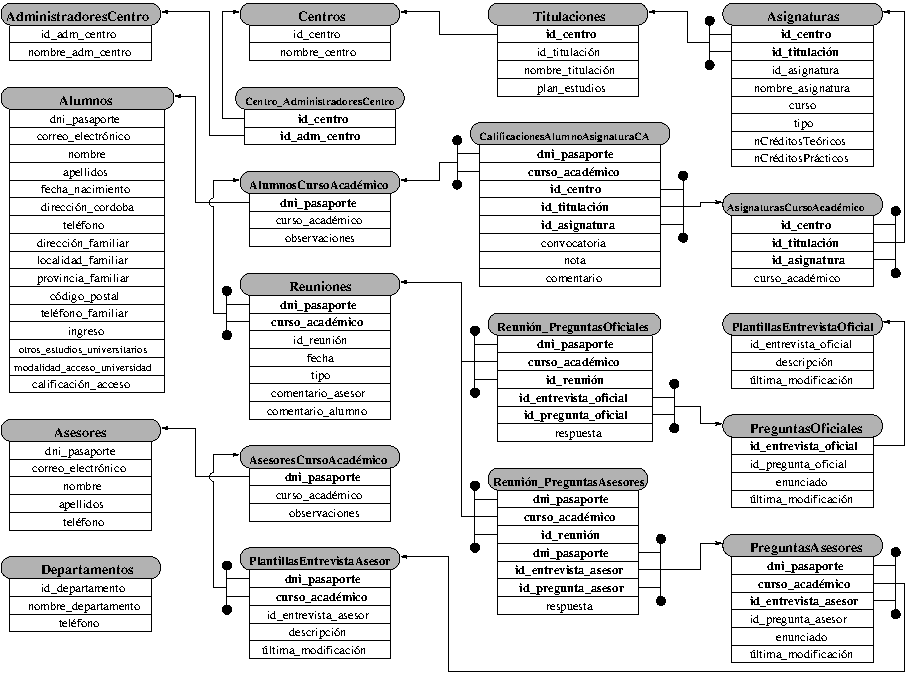
\includegraphics[]{10.Disenyo_Datos/10.5.Diagrama_Relacional/diagramaRelacional.pdf}
            \caption{Diagrama Relacional.}
            \label{diagramaRelacional}
            \end{center}
         \end{figure}

      \section{Definición Sintáctica}

   \subsection{Tabla Centros}

      \paragraph{}Esta tabla se obtiene a través del tipo de entidad
      \textit{Centro}, tomando los atributos de ésta (regla
      RTECAR-1\footnote{Según Luque Ruiz et al. \cite{luqueRuiz}, regla
      RTECAR-1: \textit{``Todos los tipos de entidad presentes en el esquema
      conceptual se transformarán en tablas o relaciones en el esquema
      relacional manteniendo el número y tipo de atributos, así como la
      característica de identificador de estos atributos.''}}).

      \paragraph{}La clave principal de esta tabla es el atributo
      \textit{id\_centro}.

      \paragraph{}La tabla \textit{Centros} queda de la siguiente forma:

      \begin{description}
         \item[Centros] \begin{flushleft}(\underline{id\_centro},
         \textsc{nombre\_centro})\end{flushleft}
      \end{description}
\subsection{Tabla AdministradoresCentro}

  \paragraph{}Esta tabla se encuentra en FNBC, ya que cada determinante
  funcional es una clave candidata de la relación.

  \paragraph{}Existen dos dependencias funcionales, la que forma la clave
  primaria de la relación con el resto de atributos y, por otro lado, la que
  forma la clave alterna con el resto de atributos de la relación.

  \begin{center}
    \begin{minipage}{3.7cm}{\begin{flushright}\begin{tabular}{ | c | }
                  \hline
                  id\_adm\_centro \\
                  \hline
                 \end{tabular}\end{flushright} }
    \end{minipage}
    \begin{minipage}{0.7cm}{$\longrightarrow$}
    \end{minipage}
    \begin{minipage}{5.9cm}{\begin{tabular}{ | c | }
                  \hline
                  correo\_electrónico \\
                  nombre\_adm\_centro \\
                  \hline
                 \end{tabular} }
    \end{minipage}
  \end{center}

  \begin{center}
    \begin{minipage}{3.7cm}{\begin{flushright}\begin{tabular}{ | c | }
                  \hline
                  correo\_electrónico \\
                  \hline
                 \end{tabular}\end{flushright} }
    \end{minipage}
    \begin{minipage}{0.7cm}{$\longrightarrow$}
    \end{minipage}
    \begin{minipage}{5.9cm}{\begin{tabular}{ | c | }
                  \hline
                  id\_adm\_centro \\
                  nombre\_adm\_centro \\
                  \hline
                 \end{tabular} }
    \end{minipage}
  \end{center}
   \subsection{Tabla Titulaciones}

      \paragraph{}Esta tabla se obtiene a través del tipo de entidad
      \textit{Titulación}, tomando los atributos de ésta (regla RTECAR-1).
      Además, mantiene una referencia con la tabla \textit{Centro} a través
      del atributo \textit{id\_centro} (regla RTECAR-3.1).

      \paragraph{}La clave principal de la tabla se compone con la agregación de
      los atributos \textit{id\_centro} e \textit{id\_titulación}. Posee una
      clave alterna que será la formada por la agregación de los atributos
      \textit{id\_centro}, \textit{nombre\_titulación} y
      \textit{plan\_estudios}.

      \paragraph{}La tabla \textit{Titulaciones} queda de la siguiente forma:

      \begin{description}
         \item[Titulaciones] \begin{flushleft}(\underline{\textbf{ID\_CENTRO},
         id\_titulación}, \textsc{nombre\_titulación},
         \textsc{plan\_estudios})\end{flushleft}
      \end{description}

\subsection{Tabla Asignaturas}

  \paragraph{}Esta tabla se encuentra en FNBC, ya que cada determinante
  funcional es una clave candidata de la relación.

  \paragraph{}Existen dos dependencias funcionales, la que forma la clave
  primaria de la relación con el resto de atributos y, por otro lado, la que
  forma la clave alterna con el resto de atributos de la relación.

 \begin{center}
    \begin{minipage}{4.2cm}{\begin{flushright}\begin{tabular}{ | c | }
                  \hline
                  (id\_centro + \\
                  id\_titulación + \\
                  id\_asignatura) \\
                  \hline
                 \end{tabular}\end{flushright} }
    \end{minipage}
    \begin{minipage}{0.7cm}{$\longrightarrow$}
    \end{minipage}
    \begin{minipage}{5.9cm}{\begin{tabular}{ | c | }
                  \hline
                  nombre\_asignatura \\
                  curso \\
                  tipo \\
                  nCréditosTeóricos \\
                  nCréditosPrácticos \\
                  \hline
                 \end{tabular} }
    \end{minipage}
  \end{center}

  \begin{center}
    \begin{minipage}{4.2cm}{\begin{tabular}{ | c | }
                  \hline
                  (id\_centro + \\
                  id\_titulación + \\
                  nombre\_asignatura) \\
                  \hline
                 \end{tabular} }
    \end{minipage}
    \begin{minipage}{0.7cm}{$\longrightarrow$}
    \end{minipage}
    \begin{minipage}{5.9cm}{\begin{tabular}{ | c | }
                  \hline
                  id\_asignatura \\
                  curso \\
                  tipo \\
                  nCréditosTeóricos \\
                  nCréditosPrácticos \\
                  \hline
                 \end{tabular} }
    \end{minipage}
  \end{center}

\subsection{Tabla AsignaturasCursoAcadémico}

  \paragraph{}Esta tabla se encuentra en FNBC puesto que el único
  determinante funcional existente es el propio identificador principal
  de la tabla.

 \begin{center}
    \begin{minipage}{4.2cm}{\begin{flushright}\begin{tabular}{ | c | }
                  \hline
                  (id\_centro + \\
                  id\_titulación + \\
                  id\_asignatura + \\
                  curso\_académico) \\
                  \hline
                 \end{tabular}\end{flushright} }
    \end{minipage}
    \begin{minipage}{0.7cm}{$\longrightarrow$}
    \end{minipage}
    \begin{minipage}{5.9cm}{\begin{tabular}{ | c | }
                  \hline
                  \\
                  \hline
                 \end{tabular} }
    \end{minipage}
  \end{center}

   \subsection{Tabla Departamentos}

      \paragraph{}Esta tabla se obtiene a través del tipo de entidad
      \textit{Departamento}, tomando los atributos de ésta (regla RTECAR-1).

      \paragraph{}La clave principal de esta tabla es el atributo
      \textit{id\_departamento}. Posee una clave alterna que será la formada por
      el atributo \textit{nombre\_departamento}.

      \paragraph{}La tabla \textit{Departamentos} queda de la siguiente forma:

      \begin{description}
         \item[Departamentos] \begin{flushleft}(\underline{id\_departamento},
         \textsc{nombre\_departamento}, teléfono)\end{flushleft}
      \end{description}

\subsection{Tabla Asesores}

  \paragraph{}Esta tabla se encuentra en FNBC, ya que cada determinante
  funcional es una clave candidata de la relación.

  \paragraph{}Existen dos dependencias funcionales, la que forma la clave
  primaria de la relación con el resto de atributos y, por otro lado, la que
  forma la clave alterna con el resto de atributos de la relación.

  \begin{center}
    \begin{minipage}{3.7cm}{\begin{flushright}\begin{tabular}{ | c | }
                  \hline
                  dni\_pasaporte \\
                  \hline
                 \end{tabular}\end{flushright} }
    \end{minipage}
    \begin{minipage}{0.7cm}{$\longrightarrow$}
    \end{minipage}
    \begin{minipage}{5.9cm}{\begin{tabular}{ | c | }
                  \hline
                  correo\_electrónico \\
                  nombre \\
                  apellidos \\
                  teléfono \\
                  \hline
                 \end{tabular} }
    \end{minipage}
  \end{center}

  \begin{center}
    \begin{minipage}{3.7cm}{\begin{tabular}{ | c | }
                  \hline
                  correo\_electrónico \\
                  \hline
                 \end{tabular} }
    \end{minipage}
    \begin{minipage}{0.7cm}{$\longrightarrow$}
    \end{minipage}
    \begin{minipage}{5.9cm}{\begin{tabular}{ | c | }
                  \hline
                  dni\_pasaporte \\
                  nombre \\
                  apellidos \\
                  teléfono \\
                  \hline
                 \end{tabular} }
    \end{minipage}
  \end{center}

   \subsection{Tabla AsesoresCursoAcadémico}

      \paragraph{}Esta tabla se obtiene a través del tipo de entidad
      \textit{Asesor Curso Académico}, tomando los atributos de ésta (regla
      RTECAR-1). Además, mantiene una referencia con la tabla \textit{Asesor}, a
      través del atributo \textit{dni\_pasaporte} y otra referencia con la tabla
      \textit{Departamento}, a través del atributo \textit{id\_departamento}
      (regla RTECAR-3.1).

      \paragraph{}La clave principal de la tabla está compuesta por la
      agregación de los atributos \textit{dni\_pasaporte} y
      \textit{curso\_académico}.

      \paragraph{}La tabla \textit{AlumnosCursoAcadémico} queda de la siguiente
      forma:

      \begin{description}
         \item[AsesoresCursoAcadémico] \begin{flushleft}(\underline{\textbf{dni\_pasaporte},
         curso\_académico}, observaciones, \textbf{id\_departamento})\end{flushleft}
      \end{description}

   \subsection{Tabla PlantillasEntrevistaAsesor}

      \paragraph{}Esta tabla se obtiene a través del tipo de entidad
      \textit{Plantilla Entrevista Asesor}, tomando los atributos de ésta
      (regla RTECAR-1). Además, mantiene una referencia con la tabla
      \textit{Asesor Curso Académico} a través de los atributos
      \textit{dni\_pasaporte} y \textit{curso\_académico} (regla RTECAR-3.1).

      \paragraph{}La clave principal de esta tabla se compone con la agregación
      de los atributos \textit{dni\_pasaporte}, \textit{curso\_académico} e
      \textit{id\_entrevista\_asesor}.

      \paragraph{}La tabla \textit{PlantillasEntrevistaAsesor} queda de la
      siguiente forma:

      \begin{description}
         \item[PlantillasEntrevistaAsesor] \begin{flushleft}(\underline{\textbf{dni\_pasaporte},
         \textbf{curso\_académico},} \underline{id\_entrevista\_asesor},
         última\_modificación)\end{flushleft}
      \end{description}

\subsection{Tabla PreguntasAsesores}

  \paragraph{}Esta tabla se encuentra en FNBC puesto que el único determinante
  funcional existente es el identificador principal y todas las dependencias
  funcionales con el resto de atributos son completas.

  \begin{center}
    \begin{minipage}{4.5cm}{\begin{flushright}\begin{tabular}{ | c | }
                  \hline
                  (dni\_pasaporte + \\
                  curso\_académico + \\
                  id\_entrevista\_asesor + \\
                  id\_pregunta\_asesor) \\
                  \hline
                 \end{tabular}\end{flushright} }
    \end{minipage}
    \begin{minipage}{0.7cm}{$\longrightarrow$}
    \end{minipage}
    \begin{minipage}{5.9cm}{\begin{tabular}{ | c | }
                  \hline
                  enunciado \\
                  última\_modificación \\
                  \hline
                 \end{tabular} }
    \end{minipage}
  \end{center}

\subsection{Tabla Alumnos}

  \paragraph{}Esta tabla se encuentra en FNBC, ya que cada determinante
  funcional es una clave candidata de la relación.

  \paragraph{}Existen dos dependencias funcionales, la que forma la clave
  primaria de la relación con el resto de atributos y, por otro lado, la que
  forma la clave alterna con el resto de atributos de la relación.

  \begin{center}
    \begin{minipage}{3.7cm}{\begin{flushright}\begin{tabular}{ | c | }
                  \hline
                  dni\_pasaporte \\
                  \hline
                 \end{tabular}\end{flushright} }
    \end{minipage}
    \begin{minipage}{0.7cm}{$\longrightarrow$}
    \end{minipage}
    \begin{minipage}{5.9cm}{\begin{tabular}{ | c | }
                  \hline
                  correo\_electrónico \\
                  nombre \\
                  apellidos \\
                  fecha\_nacimiento \\
                  dirección\_córdoba \\
                  teléfono \\
                  dirección\_familiar \\
                  localidad\_familiar \\
                  provincia\_familiar \\
                  código\_postal \\
                  teléfono\_familiar \\
                  ingreso \\
                  otros\_estudios\_universitarios \\
                  modalidad\_acceso\_universidad \\
                  calificación\_acceso \\
                  \hline
                 \end{tabular} }
    \end{minipage}
  \end{center}

  \begin{center}
    \begin{minipage}{3.7cm}{\begin{tabular}{ | c | }
                  \hline
                  correo\_electrónico \\
                  \hline
                 \end{tabular} }
    \end{minipage}
    \begin{minipage}{0.7cm}{$\longrightarrow$}
    \end{minipage}
    \begin{minipage}{5.9cm}{\begin{tabular}{ | c | }
                  \hline
                  dni\_pasaporte \\
                  nombre \\
                  apellidos \\
                  fecha\_nacimiento \\
                  dirección\_córdoba \\
                  teléfono \\
                  dirección\_familiar \\
                  localidad\_familiar \\
                  provincia\_familiar \\
                  código\_postal \\
                  teléfono\_familiar \\
                  ingreso \\
                  otros\_estudios\_universitarios \\
                  modalidad\_acceso\_universidad \\
                  calificación\_acceso \\
                  \hline
                 \end{tabular} }
    \end{minipage}
  \end{center}

   \subsection{Tabla AlumnosCursoAcadémico}

      \paragraph{}Esta tabla se obtiene a través del tipo de entidad
      \textit{Alumno Curso Académico}, tomando los atributos de ésta (regla
      RTECAR-1). Además, mantiene una referencia con la tabla \textit{Alumno} a
      través del atributo \textit{dni\_pasaporte} y con la
      tabla \textit{Asesor Curso Académico} a través de los atributos
      \textit{dni\_pasaporte} y \textit{curso\_académico} (regla RTECAR-3.1).
      Nótese que para diferenciar los atributos \textit{dni\_pasaporte} de las
      entidades \textit{Alumno Curso Académico} y \textit{Asesor Curso
      Académico} se renombrarán a \textit{dni\_pasaporte\_alumno} y
      \textit{dni\_pasaporte\_asesor}, respectivamente. Además, es necesario
      indicar que el atributo \textit{curso\_académico} que se hereda de la
      entidad \textit{Asesor Curso Académico} no se representa en esta tabla.
      Esto es debido a que dicho atributo debe coincidir con el atributo del
      mismo nombre ya existente en esta tabla, por la propia naturaleza de la
      interrelación.

      \paragraph{}La clave principal de la tabla está compuesta por la
      agregación de los atributos \textit{dni\_pasaporte} y
      \textit{curso\_académico}.

      \paragraph{}La tabla \textit{AlumnosCursoAcadémico} queda de la siguiente
      forma:

      \begin{description}
         \item[AlumnosCursoAcadémico] \begin{flushleft}(\underline{
         \textbf{dni\_pasaporte\_alumno}, curso\_académico}, observaciones,
         \textbf{dni\_pasaporte\_asesor})\end{flushleft}
      \end{description}

   \subsection{Tabla CalificacionesAlumnoAsignaturaCA}

      \paragraph{}Esta tabla se obtiene a través del tipo de entidad
      \textit{Calificación Alumno Asignatura CA}, tomando los atributos de ésta
      (regla RTECAR-1). Además, mantiene una referencia con la tabla
      \textit{Asignatura Curso Académico} a través de los atributos
      \textit{id\_centro}, \textit{id\_titulación}, \textit{id\_asignatura} y
      \textit{curso\_académico} (regla RTECAR-3.1) y con la tabla
      \textit{Alumno Curso Académico} a través del atributo
      \textit{dni\_pasaporte}(regla RTECAR-3.1). Es necesario puntualizar que el
      atributo \textit{curso\_académico} del tipo de entidad \textit{Alumno Curso
      Académico} no se tiene en cuenta, ya que se está haciendo referencia al
      atributo del mismo nombre del tipo de entidad \textit{Asignatura Curso
      Académico}, que contiene, forzosamente, la misma información.

      \paragraph{}La clave principal de esta tabla se compone con la agregación
      de los atributos \textit{dni\_pasaporte}, \textit{curso\_académico},
      \textit{id\_centro}, \textit{id\_titulación}, \textit{id\_asignatura} y
      \textit{convocatoria}.

      \paragraph{}La tabla \textit{AsignaturasCursoAcadémico} queda de la
      siguiente forma:

      \begin{description}
         \item[CalificacionesAlumnoAsignaturaCA] \begin{flushleft}(
         \underline{\textbf{dni\_pasaporte}, \textbf{curso\_académico},}
         \underline{\textbf{id\_centro}, \textbf{id\_titulación},
         \textbf{id\_asignatura}, convocatoria}, nota, comentario)
         \end{flushleft}
      \end{description}

   \subsection{Tabla PlantillasEntrevistaOficial}

      \paragraph{}Esta tabla se obtiene a través del tipo de entidad
      \textit{Plantilla Entrevista Oficial}, tomando los atributos de ésta
      (regla RTECAR-1).

      \paragraph{}La clave principal de esta tabla es el atributo
      \textit{id\_entrevista\_oficial}.

      \paragraph{}La tabla \textit{PlantillasEntrevistaOficial} queda de la
      siguiente forma:

      \begin{description}
         \item[PlantillasEntrevistaOficial] \begin{flushleft}(\underline{id\_entrevista\_oficial}, última\_modificación)\end{flushleft}
      \end{description}

   \subsection{Tabla PreguntasOficiales}

      \paragraph{}Esta tabla se obtiene a través del tipo de entidad
      \textit{Pregunta Oficial}, tomando los atributos de ésta
      (regla RTECAR-1). Además, mantiene una referencia con la tabla
      \textit{Plantilla Entrevista Oficial} a través del atributo
      \textit{id\_entrevista\_oficial} (regla RTECAR-3.1).

      \paragraph{}La clave principal de esta tabla se compone con la agregación
      de los atributos \textit{id\_entrevista\_oficial} e
      \textit{id\_pregunta\_oficial}.

      \paragraph{}La tabla \textit{PreguntasOficiales} queda de la
      siguiente forma:

      \begin{description}
         \item[PreguntasOficiales] \begin{flushleft}(\underline{\textbf{id\_entrevista\_oficial},
         id\_pregunta\_oficial})\end{flushleft}
      \end{description}

   \subsection{Tabla Reuniones}

      \paragraph{}Esta tabla se obtiene a través del tipo de entidad
      \textit{Reunión}, tomando los atributos de ésta (regla RTECAR-1).
      Además, mantiene una referencia con la tabla \textit{Alumno Curso
      Académico} a través de los atributos \textit{dni\_pasaporte} y
      \textit{curso\_académico} (regla RTECAR-3.1).

      \paragraph{}La clave principal de esta tabla se compone con la agregación
      de los atributos \textit{dni\_pasaporte}, \textit{curso\_académico} e
      \textit{id\_reunión}.

      \paragraph{}La tabla \textit{Reuniones} queda de la siguiente forma:

      \begin{description}
         \item[Reuniones] \begin{flushleft}(\underline{\textbf{dni\_pasaporte},
         \textbf{curso\_académico}, id\_reunión}, fecha, tipo,
         comentario\_asesor, comentario\_alumno)\end{flushleft}
      \end{description}

   \subsection{Tabla Centro\_AdministradoresCentro}

      \paragraph{}Esta tabla surge de la interrelación AC-C, existente entre
      los tipos de entidad \textit{Administrador Centro} y \textit{Centro}
      (regla RTECAR-4\footnote{Según Luque Ruiz et al. \cite{luqueRuiz}, regla
      RTECAR-4: \textit{En un tipo de
      interrelación binaria N:N cada tipo de entidad se transforma en una tabla
      por aplicación de la regla RTECAR-1 y se genera una nueva tabla para
      representar al tipo de interrelación. Esta tabla estará formada por los
      identificadores de los tipos de entidad que intervienen en el tipo
      de interrelación y por todos los atributos asociados al tipo de
      interrelación. La clave principal de esta tabla será la agregación de los
      atributos identificadores correspondientes a los tipos de entidad que
      intervienen en el tipo de interrelación.}}), tomando los atributos de
      ésta. Gracias a esta interrelación, se podrá conocer los diferentes
      administradores de existen en un centro.

      \paragraph{}La clave principal de esta tabla la forman la agregación de
      los atributos \textit{id\_centro} e \textit{id\_adm\_centro}. Estos
      atributos son a su vez claves foráneas.

      \paragraph{}La tabla \textit{Centro\_AdministradoresCentro} queda de la
      siguiente forma:

      \begin{description}
         \item[Centro\_AdministradoresCentro] \begin{flushleft}(\underline{\textbf{id\_centro},
         \textbf{id\_adm\_centro}})\end{flushleft}
      \end{description}
% \subsection{Tabla Reunión\_PreguntasAsesores}

  \paragraph{}Esta tabla se encuentra en FNBC puesto que el único determinante
  funcional existente es el identificador principal y todas las dependencias
  funcionales con el resto de atributos son completas.

  \begin{center}
    \begin{minipage}{5.0cm}{\begin{flushright}\begin{tabular}{ | c | }
                  \hline
                  (dni\_pasaporte\_alumno + \\
                  curso\_académico + \\
                  id\_reunión + \\
                  dni\_pasaporte\_asesor + \\
                  id\_entrevista\_asesor + \\
                  id\_pregunta\_asesor) \\
                  \hline
                 \end{tabular}\end{flushright} }
    \end{minipage}
    \begin{minipage}{0.7cm}{$\longrightarrow$}
    \end{minipage}
    \begin{minipage}{5.9cm}{\begin{tabular}{ | c | }
                  \hline
                  respuesta \\
                  \hline
                 \end{tabular} }
    \end{minipage}
  \end{center}

\subsection{Tabla Reunión\_PreguntasOficiales}

  \paragraph{}Esta tabla se encuentra en FNBC puesto que el único determinante
  funcional existente es el identificador principal y todas las dependencias
  funcionales con el resto de atributos son completas.

  \begin{center}
    \begin{minipage}{4.4cm}{\begin{flushright}\begin{tabular}{ | c | }
                  \hline
                  (dni\_pasaporte + \\
                  curso\_académico + \\
                  id\_reunión + \\
                  id\_entrevista\_oficial + \\
                  id\_pregunta\_oficial) \\
                  \hline
                 \end{tabular}\end{flushright} }
    \end{minipage}
    \begin{minipage}{0.7cm}{$\longrightarrow$}
    \end{minipage}
    \begin{minipage}{5.9cm}{\begin{tabular}{ | c | }
                  \hline
                  respuesta \\
                  \hline
                 \end{tabular} }
    \end{minipage}
  \end{center}


   \chapter{Diseño arquitectónico}

   \chapter{Diseño procedimental}

   \chapter{Diseño de la interfaz}

   \chapter{Pruebas}\label{pruebas}

   \chapter{Resultados}

   \chapter{Conclusiones}

   \chapter{Futuras mejoras}
    \paragraph{}En este capítulo se van a proponer las posibles futuras mejoras
a las que puede ser sometida la aplicación desarrollada en el presente
proyecto fin de carrera. Las futuras mejoras son las siguientes:

\begin{itemize}
  \item Integrar el expediente académico de los alumnos en el sistema
  desarrollado. Para ello, será necesario realizar la conexión con la base de
  datos de Sigma \cite{sigma}, para lo cual se requeriría la autorización
  correspondiente de la Universidad de Córdoba.
  \item Mejorar la comunicación entre los distintos usuarios de la aplicación,
  sobretodo entre asesores y alumnos. Para ello, sería deseable que se pudieran
  dejar mensajes en el sistema para que, por ejemplo, se pudiera realizar
  convocatorias públicas a los alumnos.
  \item Organizar las preguntas de las plantillas por bloques. Esto facilitaría
  la organización y legibilidad de las entrevistas realizadas por los asesores
  a los alumnos. Se podrían agrupar por preguntas docentes, salidas
  profesionales, entorno social, etc.
  \item Mejorar la gestión de las preguntas de las plantillas, distinguiéndolas
  por el tipo de respuesta que tengan, por ejemplo:
  \begin{itemize}
    \item Numérica.
    \item Lógica (Sí o No).
    \item Descriptiva.
  \end{itemize}
  \item Permitir la inclusión en el sistema de plantillas de centro. De esta
  manera, sería más fácil y homogéneo la realización de entrevistas que afecten
  a un centro en particular.
\end{itemize}




   \listoffigures

   \begin{thebibliography}{xx}

\bibitem{debian} \textbf{Debian GNU/Linux}, 2009.\\
         Sitio web oficial del sistema operativo.\\
         url: \url{http://www.debian.org/}
         [Consulta: 20 junio 2009].
\bibitem{django} \textbf{Django}, 2009.\\
         Sitio oficial del proyecto.\\
         url: \url{http://www.djangoproject.com/}
         [Consulta: 20 junio 2009].
\bibitem{kate} \textbf{Kate}, 2009.\\
         Sitio oficial del editor de textos.\\
         url: \url{http://kate-editor.org/}
         [Consulta: 20 junio 2009].
\bibitem{kile} \textbf{Kile}, 2009.\\
         Sitio oficial del editor de Tex/Latex.\\
         url: \url{http://kile.sourceforge.net/}
         [Consulta: 20 junio 2009].
\bibitem{latex} \textbf{Latex}, 2009.\\
         Sitio oficial del proyecto \LaTeX.\\
         url: \url{http://www.latex-project.org/}
         [Consulta: 20 junio 2009].
\bibitem{microsoft} \textbf{Microsoft}, 2009.\\
         Sitio oficial de la compañía.\\
         url: \url{http://www.microsoft.com/}
         [Consulta: 20 junio 2009].
\bibitem{mysql} \textbf{MySQL}, Sun Microsystems, 2009.\\
         Sitio oficial del sistema gestor de bases de datos.\\
         url: \url{http://www.mysql.com/}
\bibitem{oracle} \textbf{Oracle}, 2009.\\
         Sitio oficial del sistema gestor de bases de datos.\\
         url: \url{http://www.oracle.com/}
         [Consulta: 20 junio 2009].
\bibitem{peterChen} \textbf{Peter Pin-Shan S. Chen}, 1976.\\
         The Entity-Relationship Model: Toward a Unified View of Data. \\
         ACM Transactions on Database Systems. Páginas 9-36.
         ISSN:0362-5915.
\bibitem{php} \textbf{PHP}, 2009.\\
         Sitio oficial del lenguaje.\\
         url: \url{http://www.php.net/}
         [Consulta: 20 junio 2009].
\bibitem{postgresql} \textbf{PostgreSQL}, 2009.\\
         Sitio oficial del sistema gestor de bases de datos.\\
         url: \url{http://www.postgresql.org/}
         [Consulta: 20 junio 2009].
\bibitem{python} \textbf{Python}, 2009.\\
         Sitio oficial del lenguaje.\\
         url: \url{http://www.python.org/}
         [Consulta: 20 junio 2009].
\bibitem{ruby} \textbf{Ruby}, 2009.\\
         Sitio oficial del lenguaje.\\
         url: \url{http://www.ruby-lang.org/}
         [Consulta: 20 junio 2009].
\bibitem{subversion} \textbf{Subversion} , 2009.\\
         Sitio oficial del sistema de control de versiones.\\
         url: \url{http://subversion.tigris.org/}
         [Consulta: 20 junio 2009].
\bibitem{wikipedia} \textbf{Wikipedia}, 2009.\\
         Sitio oficial del proyecto.\\
         url: \url{http://www.wikipedia.org/}
         [Consulta: 20 junio 2009].
 \end{thebibliography}

   \appendix
   \chapter{Reglamento regulador de la figura del Asesor Académico}\label{a1}
   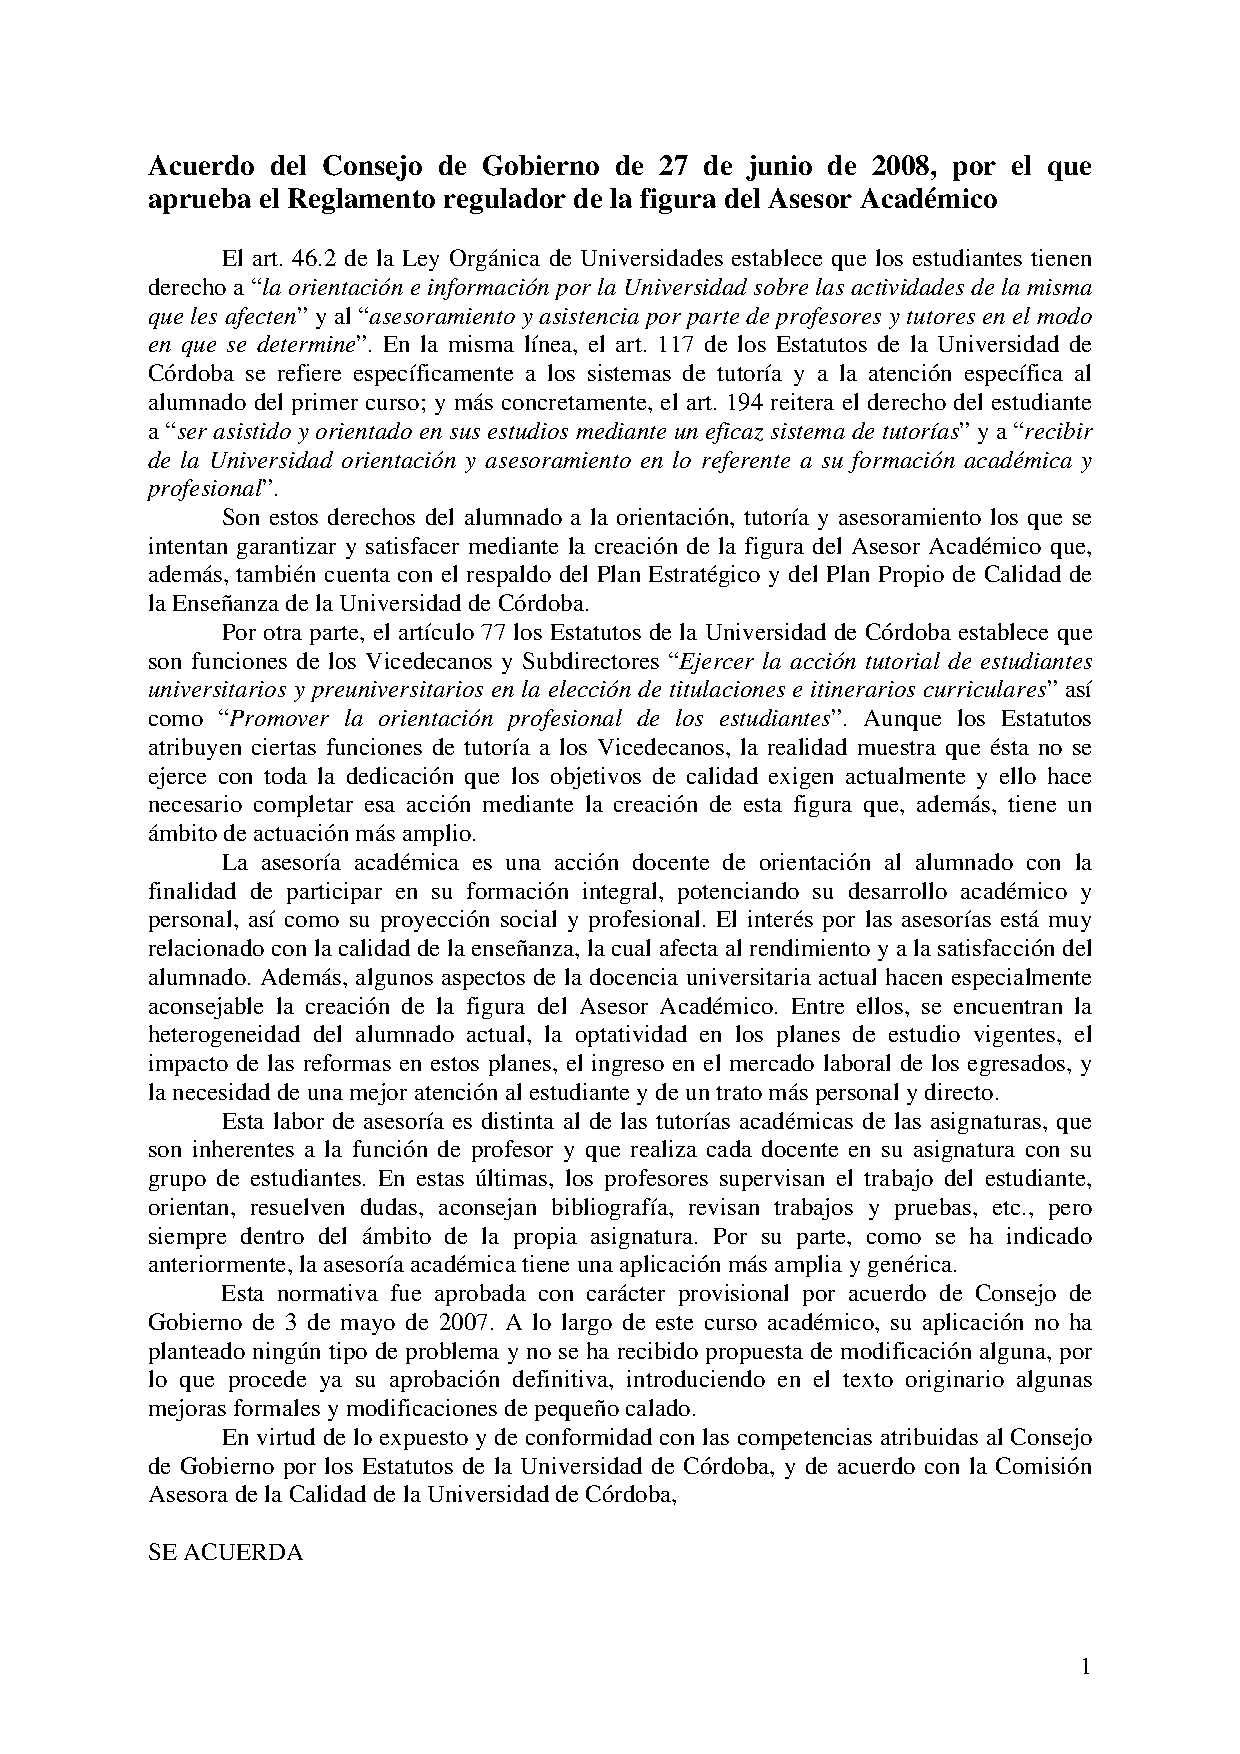
\includepdf[pages={-},lastpage=4]{Anexos/ReglamentoAsesoriaAcademica.pdf}
\end{document}
